\documentclass[
  12pt,  %% Requirement 1.1.2 Typeface size and style
  oneside,  %% Requirement 1.1.3 Margins
]
{book}

%% Requirement 1.1.1 Double space
\usepackage{setspace}
\doublespacing

%% Requirement 1.1.2 Typeface size and style
\usepackage{titlesec}
%% HACK In titlesec version 2.10.1 (the version provided by Ubuntu 16.04) there
%% is a bug that removes section numbers from section headings. The following
%% code fixes that regression. If titlesec version 2.10.2 or later is
%% available, this code can be safely removed. See
%% <http://tex.stackexchange.com/a/300259/4430>.
\usepackage{etoolbox}
\makeatletter
\patchcmd{\ttlh@hang}{\parindent\z@}{\parindent\z@\leavevmode}{}{}
\patchcmd{\ttlh@hang}{\noindent}{}{}{}
\makeatother
%% END HACK
\titleformat*{\section}{\normalsize\bfseries}
\titleformat*{\subsection}{\normalsize\bfseries}
\titleformat*{\subsubsection}{\normalsize\bfseries}
\titleformat*{\paragraph}{\normalsize\bfseries}
\titleformat*{\subparagraph}{\normalsize\bfseries}

\usepackage{calc}
\usepackage[
  %% Requirement 1.1.3 Margins
  top=1.5in,
  left=1.5in,
  right=1in,
  bottom=1in,
  %% Requirement 1.1.5 Page numbering, page number placement, ...
  headsep={0.5in - 12pt},
]{geometry}

%% Requirement 1.1.5 Page numbering, page number placement, ...
%%
%% HACK In order to start page numbering on the title page, we need to redefine
%% it so it does not reset the page number after it. See
%% <http://tex.stackexchange.com/a/172005/4430>.
\makeatletter
\renewenvironment{titlepage}
 {%
   \@restonecolfalse\newpage
   \thispagestyle{empty}%
 }
 {%
   \newpage
 }
\makeatother

%\usepackage{amsmath}
%\usepackage{amssymb}
%% This must come before hyperref.
%\usepackage{amsthm}
%% This is strongly recommended by biblatex.
\usepackage[english]{babel}
\usepackage[backend=biber]{biblatex}
\usepackage[T1]{fontenc}
%% This must come before csquotes.
\usepackage[utf8]{inputenc}
\usepackage{lmodern}
%% This is strongly recommended by biblatex.
\usepackage{csquotes}
%% This must come before hyperref.
%\usepackage{thmtools}
%% This must come before complexity.
\usepackage{hyperref}
%\usepackage{complexity}
\usepackage[final]{microtype}
%\usepackage{tikz}

\LoadMicrotypeFile{cmr}
\SetProtrusion
    [load=lmr-T1]
    {encoding=T1, family=lmr}
    {
      \textquotedblright = {,1000},
      \textquotedblleft = {1000,},
      {'} = {,1000},
      {,} = {,1000},
      {:} = {,1000},
      {;} = {,1000},
      {.} = {,1000}
    }

%% Set the title and author of the PDF file.
\hypersetup{
  pdftitle={Parallelism with limited nondeterminism},
  pdfauthor={Jeffrey Finkelstein}
}

%% Declare the bibliography file.
%\addbibresource{dissertation.bib}

%% Declare theorem-like environments.
%\declaretheorem[numberwithin=section]{theorem}

%% Custom commands are declared here.
\newcommand{\todo}[1]{\textbf{TODO #1}}
\newcommand{\dash}{\textnormal{-}}

%% Define the author, title, and date for the document.
\title{Parallelism with limited nondeterminism}
\author{Jeffrey~Finkelstein}

\begin{document}

%% Requirement 1.1.6 Order of pagination
\frontmatter
\begin{titlepage}
  \begin{center}

    \uppercase{Boston University}\\
    \uppercase{Graduate School of Arts and Sciences}

    \vspace{8ex}

    Dissertation

    \vspace{10ex}

    \textbf{\uppercase{Parallelism with limited nondeterminism}}

    \vspace{10ex}

    by

    \vspace{8ex}

    \textbf{\uppercase{Jeffrey Finkelstein}}

    \vspace{5ex}
    B.S., Tufts University, 2010

    \vspace{22ex}

    Submitted in partial fulfillment of the\\
    requirements for the degree of\\
    Doctor of Philosophy\\
    2017
  \end{center}
\end{titlepage}

\newenvironment{copyrightpage}
  {%
  \thispagestyle{empty}%
  \setlength{\parindent}{0pt}%
  \null
  \vfill
  }
  {\newpage}

\begin{copyrightpage}
  Copyright 2017 \uppercase{Jeffrey Finkelstein}.\\
  This work is licensed under the Creative Commons Attribution-ShareAlike 4.0\\ International License. To view a copy of this license,\\ visit \url{http://creativecommons.org/licenses/by-sa/4.0/}.
\end{copyrightpage}

\newenvironment{readerspage}
  {\thispagestyle{empty}}
  {\newpage}

\begin{readerspage}
  \begin{center}
    Approved by
  \end{center}
  \vspace{21ex}
  \renewcommand{\arraystretch}{0.6}
  \begin{tabular}{l p{4.5in}}
    First Reader & \hrulefill \\
    & Steven Homer, Ph.D. \\
    & Professor of Computer Science \\[13ex]

    Second Reader & \hrulefill \\
    & Benjamin Hescott, Ph.D. \\
    & Assistant Professor of Computer Science \\
    & Tufts University \\[11ex]

    Third Reader & \hrulefill \\
    & Péter Gács, Ph.D. \\
    & Professor of Computer Science \\
    & Boston University
  \end{tabular}
\end{readerspage}

%\newenvironment{dedication}
  {%
    \thispagestyle{plain}%
    \vspace*{\stretch{1}}%
    \raggedleft%
    \itshape%
  }
  {%
    \vspace{\stretch{1.618}}%
    \clearpage%
  }

\begin{dedication}
  To my parents.
\end{dedication}

%\input{acknowledgments}
\newenvironment{abstractpage}
  {\thispagestyle{plain}}
  {}

\begin{abstractpage}
  \begin{center}
    \textbf{\uppercase{Parallelism with limited nondeterminism}}\\
    \textbf{\uppercase{Jeffrey Finkelstein}}\\
    Boston University Graduate School of Arts and Sciences, 2017\\
    Major Professor: Steven Homer, Ph.D., Professor of Computer Science
  \end{center}
  \begin{center}
    ABSTRACT
  \end{center}
  % % Foreword %
  %
  % %% Context (anyone - why now?) %%
  %
  % What is the current situation, and why is the need so important?
  %
  Computational complexity theory studies which computational problems can be solved with limited access to resources.
  The past fifty years have seen a focus on the relationship between intractable problems and efficient algorithms.
  %
  % %% Need (readers - why you?) %%
  %
  % Why is this relevant to the reader, and why does something need to be done?
  % (Also reference relevant existing work.)
  %
  However, the relationship between inherently sequential problems and highly parallel algorithms has not been well studied.
  Are there efficient but inherently sequential problems that admit some relaxed form of highly parallel algorithm?
  %
  % %% Task (author - why me?) %%
  %
  % What was undertaken to address the need?
  %
  In this dissertation, we develop the theory of structural complexity around this relationship for three common types of computational problems.
  %
  % %% Object (document - why this document?) %%
  %
  % What does this document cover?
  %

  %
  % % Summary %
  %
  % %% Findings (author - what?)
  %
  % What did the work reveal when performing the task?
  %
  Specifically, we show tradeoffs between time, nondeterminism, and parallelizability.
  By clearly defining the notions and complexity classes that capture our intuition for parallelizable and sequential problems, we create a comprehensive framework for rigorously proving parallelizability and non-parallelizability of computational problems.
  %
  % %% Conclusion (readers - so what?)
  %
  % What did the findings mean for the audience?
  %
  The current growth of multiprocessor systems highlights the need to consider whether otherwise tractable problems can be effectively parallelized, and this framework provides the means to prove it.
  %
  % %% Perspective (anyone - what now?)
  %
  % What should be done next?
  The views adopted by this dissertation---alternate approaches to solving sequential problems using approximation, limited nondeterminism, and parameterization---can be applied practically throughout computer science.
\end{abstractpage}

%\input{preface}
\tableofcontents
\listoftables
\listoffigures
\chapter{List of abbreviations}

\chapter{Glossary}


\mainmatter
\chapter{Introduction}

% % Foreword %
%
% %% Context (anyone - why now?) %%
%
% What is the current situation, and why is the need so important?
%
Since parallel computing is again becoming a topic of interest in computer science, it is important to revisit the theoretical foundations of highly parallel computing.
In theoretical computer science, computational complexity studies what problems can be solved when facing limited access to resources.
With parallelism as the resource of interest, computational complexity has already classified numerous computational problems as either ``inherently sequential'' or ``parallelizable''\kern-0.45em.\kern0.45em
Inherently sequential computational problems, unlike parallizable problems, see no significant speedup when run on highly parallel computers.

Computational problems can be further classified into three types: decision problems, optimization problems, and parameterized problems.
Decision problems are of the form ``Does object $x$ have property $P$?''
Decision problems lead to the other two kinds of problems by modifying either the solution space or the resource usage bounds.
Optimization problems generalize decision problems by allowing a search for a good solution among many candidates.
Parameterized problems generalize decision problems by allowing resource bounds to depend on a parameter of the problem instance instead of simply the size.
The study of the computational complexity of both optimization problems and parameterized problems provides a more detailed view than the study of decision problems alone.

%
% %% Need (readers - why you?) %%
%
% Why is this relevant to the reader, and why does something need to be done?
% (Also reference relevant existing work.)
%
Just as there are efficient approximations for intractable optimization problems, so too are there efficient and highly parallel approximations for optimization problems that are tractable but inherently sequential.
For example, the problem of computing the optimal vector in a positive linear program---a problem relevant to distributed flow control within a network of routers---is inherently sequential, but a vector very close to the optimal one can be computed quickly in parallel.
Similarly, just as there are fixed-parameter tractable algorithms for some intractable problems, so too are there fixed-parameter parallel algorithms for some sequential parameterized problems.
For example, the problem of evaluating a Boolean circuit on a given input is inherently sequential, but the circuit can be evaluated quickly in parallel when the depth of the circuit is considered a parameter of the problem.
These facts, which require proofs, give practicioners the confidence that when faced with inherently sequential problems, all hope is not lost.

%
% %% Task (author - why me?) %%
%
% What was undertaken to address the need?
%
We develop the theory of structural complexity for highly parallel algorithms for tractable but inherently sequential problems in decision problems, optimization problems, and parameterized problems.
This area has not been well-studied, and when it has been studied, the results focus mostly on parallel algorithms for \emph{intractable} problems, %% (that is, $\NC$ algorithms for $\NP$-complete problems),
not parallel algorithms for tractable sequential problems %% (that is, $\NC$ algorithms for $\P$-complete problems)
.
%
% %% Object (document - why this document?) %%
%
% What does this document cover?
%
This dissertation proves the main theorems required for the study of the computational complexity of parallelizable versus sequential computational problems and provides the motivation and intuition to understand their significance and use.

%
% % Summary %
%
% %% Findings (author - what?)
%
% What did the work reveal when performing the task?
%
There are three main chapters in this dissertation, each of which discusses a different type of computational problem, namely decision problems, optimization problems, and parameterized problems.
Each chapter discusses the main approaches to proving the limitations of highly parallel algorithms for tractable but inherently sequential problems of the respective type.
Further, we show how adding a limited amount of nondeterminism to a highly parallel algorithm allows us to circumvent some limitations of parallelism without requiring sequential computation.

In \autoref{chp:decision}, we discuss augmenting a highly parallel algorithm for decision problems with a small amount of nondeterminism as the basis for a technique to prove inapproximability of optimization problems.
In \autoref{chp:optimization}, we define and explore the complexity classes associated with parallel approximation algorithms for inherently sequential optimization problems.
In \autoref{chp:parameterized}, we formalize the tradeoffs between time, parallelism, and nondeterminism in parameterized problems and show some connections with decision and optimization problems.

%
% %% Conclusion (readers - so what?)
%
% What did the findings mean for the audience?
%
\textbf{Add another conclusion paragraph HERE}

Under the assumption that $\NC \neq \P$, the fact that $\NNC[\poly] = \NP$ (\autocite{wolf94}) but $\NNCO \neq \NPO$ (\autoref{thm:nnconpo}) leads us to conclude that viewing a computational problem as merely a decision problem is too coarse-grained an approach---it does not give enough information about the computational complexity of the problem.
The conjecture that $\para \WNC \neq \para \WP$ if and only if $\NNC[\omega(\log n)] = \NP[\omega(\log n)]$ (\autoref{con:wncwp}) supports this view as well, if the conjecture holds.
This means that considering the complexity of decision, both parameterized and unparameterized, and of approximation independently is insufficient.
Researchers and practicioners should consider the complexity of verification in addition to the complexity of decision and optimization.

%
% %% Perspective (anyone - what now?)
%
% What should be done next?
This line of research, along with the fact that the complexity of solving a decision problem seems to have little to with the approximability or parameterized complexity of that problem, emphasizes the need to further determine the relative difficulty of computational problems with respect to the complexity of decision, verification, and approximation.
Descriptive complexity seems like a promising way of unifying the complexity analyses of the different kinds of computational problems explored here; there are descriptive complexity characterizations for classes of decision problems \autocite{immerman99}, classes of approximable optimization problems \autocite{kt93}, and classes of parameterized problems \autocite{fg06}.

\section{TODO Incorporate these diagrams somewhere}

%% We study the structural complexity of sequential versus parallel computation in decision problems, optimization problems, and parameterized problems.

\begin{minipage}[t]{0.31\linewidth}
  \centering
  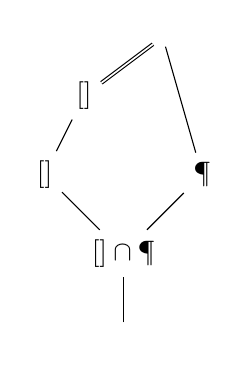
\begin{tikzpicture}
  \node at (0, 0) (nc) {$\NC$};
  \node at (0, 1) (both) {$\NNC[\polylog] \cap \P$};
  \node at (-1, 2) (nncpolylog) {$\NNC[\polylog]$};
  \node at (1, 2) (p) {$\P$};
  \node at (0.5, 3.75) (np) {$\NP$};
  \node at (-0.5, 3) (nnc) {$\NNC[\poly]$};

  \draw (nc) to (both);
  \draw (both) to (nncpolylog);
  \draw (both) to (p);
  \draw (p) to (np);
  \draw (nncpolylog) to (nnc);
  \draw[double] (nnc) to (np);
\end{tikzpicture}

\end{minipage}%
\begin{minipage}[t]{0.31\linewidth}
  \centering
  \begin{tikzpicture}
  \node at (0, 0) (nco) {$\NCO$};
  \node at (0, 1) (both) {$\ApxNCO \cap \PO$};
  \node at (-1, 2) (apxnco) {$\ApxNCO$};
  \node at (1, 2) (po) {$\PO$};
  \node at (0.5, 3.75) (npo) {$\NPO$};
  \node at (-0.5, 3) (nnco) {$\NNCO$};

  \draw (nco) to (both);
  \draw (both) to (apxnco);
  \draw (both) to (po);
  \draw (po) to (npo);
  \draw (apxnco) to (nnco);
  \draw[double] (nnco) -- (npo) node [rotate=45, midway] {\small$/$};
\end{tikzpicture}

\end{minipage}%
\begin{minipage}[t]{0.31\linewidth}
  \centering
  \begin{tikzpicture}
  \node at (0, 0) (fpnc) {$\para \NC$};
  \node at (0, 1) (both) {$\para \WNC[1] \cap \para \P$};
  \node at (-1, 2) (dontknow) {$\para \WNC[1]$};
  \node at (1, 2) (fpt) {$\para \P$};
  \node at (0.5, 3.75) (wp) {$\para \WP$};
  \node at (-0.5, 3) (wpp) {$\para \WNC$};

  \draw (fpnc) to (both);
  \draw (both) to (dontknow);
  \draw (both) to (fpt);
  \draw (fpt) to (wp);
  \draw (dontknow) to (wpp);
  \draw (wpp) to (wp);
\end{tikzpicture}

\end{minipage}

These inclusion diagrams shape how we approach all the problems in this paper.
Double lines represent equality, solid lines represent strict inequality under some reasonable complexity-theoretic assumptions, and dashed lines represent inclusions of unknown strictness or equality.
%% The fact that $\NNC[\poly] = \NP$ but $\NNCO \neq \NPO$ and $\para \WNC \neq \para \WP$ (under the assumption $\NC \neq \P$) leads us to conclude that viewing a computational problem as merely a decision problem is too coarse-grained an approach---it does not give enough information about the computational complexity of the problem.

%There is another view that we approach only indirectly in this work, the complexity of verification.
%% This is why $\NNCO$ differs from $\NPO$ and $\para \WNC$ differs from $\para \WP$: these classes take into account the complexity of verifying a solution.
%% The classes of decision problems $\NNC[\poly]$ and $\NP$ do not.

%% \todo{Descriptive complexity encompasses all of these; specifically for parallel complexity of optimization problems, see \autocite{kt93}.}

\section{TODO Make sure the introduction of each section covers these points}
We aim to show that there is a $\P$-complete problem that is also
\begin{enumerate}
\item[(D1)] not in $\NNC[\polylog]$ (\autocite[Theorem~3.9]{ncpcp} provides one unless $P \subsetneq \polyL$),
\item[(D2)] in $\NNC[\polylog]$ but not in $\NC$ (unknown),
\item[(O1)] not in $\ApxNCO$ (\autocite[Theorem~3.25]{ncapproximation} provides one unless $\NC = \P$),
\item[(O2)] in $\ApxNCO$ but not in $\NCO$ (\autocite[Theorem~3.25]{ncapproximation} provides on unless $\NC = \P$),
\item[(P1)] not in $\para \WNC[1]$ (unknown),
\item[(P2)] in $\para \WNC[1]$ but not in $\para \NC$ (unknown).
\end{enumerate}

\section{Outline}

The referenced theorems correspond to the theorems in the respective papers.

\paragraph{Decision Problems.}
Completed:
\begin{enumerate}
\item $\NC = \PCP[O(\log \log n, O(1)]$ (Theorem~3.3).
\item $\NNC[\polylog] = \PCP[O(\log \log n), \polylog]$ (Corollary~3.2).
\item $\NP = \PCP[O(\log n), O(1)]$ (Theorem~3.4).
\item negative consequences $\PCP$ hierarchy collapses (Corollary~3.6) (\emph{relates to parameterized problems})
\item consequences of $\P = \PCP[O(\log \log n), \polylog]$ (Theorem~3.9).
\end{enumerate}
To-do:
\begin{enumerate}
\item \textbf{Low priority:} Inapproximability of the High Degree Subgraph problem (Section~4) (\emph{relates to optimization problems}).
\end{enumerate}

\paragraph{Optimization problems.}

Completed:
\begin{enumerate}
\item $\NNCO$-complete problem (Theorem~3.3).
\item $\NPO$-complete problem (Corollary~3.4).
\item $\NNCO = \NPO \iff \NC = \P$ (Theorem~3.5).

\item $\PO$-complete problem (Theorems~3.8 and 3.9).
\item $(\PO \cap \NNCO)$-complete problem (Corollary~3.11).
\item $\PO \cap \NNCO = \PO \iff \NC = \P$ (Theorem~3.12).

\item $\PO \cap \NNCO$ is not closed under $\leq_m^{AP}$ reductions (Corollary~3.10).

\item Strictness of $\NNCO$ approximation hierarchy (Theorem~3.24).
\item Strictness of $\PO \cap \NNCO$ approximation hierarchy (Theorem 3.25).
\end{enumerate}
To-do:
\begin{enumerate}
\item \textbf{Low priority:} $\ApxNCO$-complete problem (Section~3.3).
\item \textbf{High priority:} descriptive complexity characterization of $\ApxNCO$ (Section~4) (\emph{relates to parameterized problems}).
\item \textbf{High priority:} reduction preserving both verification complexity and approximability.
\end{enumerate}

\paragraph{Parameterized problems.}
Completed:
\begin{enumerate}
\item Circuit value problem is $\P$-complete but in $\para \AC^{0 \uparrow}$ (Theorems~3.3 and 3.5).
\item Nonuniform circuits for proving $\NC = \NNC[i(n) \log n] \implies \para \NC = \para \WNC$.
\item $\mathcal{O} \in \ENCAS \implies p \dash \mathcal{O} \in \para \NC$ (Theorem~3.18)
\item $\para \P$-complete problems (Section~4.2).
\item Definition of $\para \WNC[t]$?
\item $\para\NC = \para \WNC[t] \iff \Pi_t\LOGTIME[i(n) \log n] \subseteq \NC^d$, if it's correct (Section~6.4).
\end{enumerate}
To-do:
\begin{enumerate}
\item \textbf{High priority:} extend \autocite[Corollary~3.8]{est15} to $\para \WNC^d \subseteq \para \P$ implies $\W[\NC^d \textsc{sat}] = \para \P$?
\item \textbf{Very high priority:} show that collapses in the inclusion chain $\para \WNC^1$ through $\para \WP$ imply corresponding collapses in decision problems? This should follow from ``Describing parameterized complexity classes'' by Flum and Grohe (Section~5.6) (\emph{relates to decision problems}).
\item \textbf{Low priority:} provide descriptive complexity characterizations of the $\para \W \mathcal{C}$ classes?
\item \textbf{High priority:} $\para \WNC^1[t] \subseteq \para \P$ if and only if a class between $\W[t] = \para \P$?
\end{enumerate}

\newcommand{\PCPcs}[5]{\PCP^{#1}_{#2, #3}\left[#4, #5\right]}
\newcommand{\loglog}{\log\log}
\newcommand{\ceil}[1]{\left\lceil{#1}\right\rceil}
\newcommand{\FSAT}{\textsc{FSat}}

\chapter{Decision problems}
\label{chp:decision}

% % Foreword %
%
% %% Context (anyone - why now?) %%
%
% What is the current situation, and why is the need so important?
%
\lettrine[loversize=0.1, lhang=0.05, findent=0.2em, nindent=0em]{O}{ne of the major successes} of the PCP Theorem, a characterization of $\NP$ as a class of computational problems that have probabilistically checkable proof systems (with polynomial-time verifiers), is that it provides a route to proving that approximating certain computationally intractable optimization problems is as difficult as solving them exactly.
%
% %% Need (readers - why you?) %%
%
% Why is this relevant to the reader, and why does something need to be done?
% (Also reference relevant existing work.)
%
The growth of multiprocessor systems in both general purpose personal computing and large-scale big data computations highlights the urgency of proving the analagous inapproximability (or approximability) of inherently sequential optimization problems by highly parallel algorithms.
However, there has been little theoretical work toward proving parallel inapproximability.
Unfortunately, the techniques used to prove the original PCP Theorem rely on the fact that $\NP$ can be interpreted as the class of languages for which there is an efficient verification procedure given a brief witness to language membership; no such obvious interpretation of $\P$ exists.

If we consider the $\P$-complete problems to be tractable but inherently sequential and $\NC$ problems to be highly parallelizable, then our guiding question is whether there is a probabilistically checkable proof (PCP) characterization of $\P$ with $\NC$ verifiers.
Such a characterization would potentially provide a path to proving parallel inapproximability.
Indeed, this question was already on the minds of researchers such as Luca~Trevisan soon after the original proof of the PCP Theorem.
\begin{quote}
  An intriguing question is whether the known non-approximability results for sequential algorithms can be improved when we restrict to $\NC$ algorithms (under the assumption that $\P \neq \NC$).
  A possible way may be to devise \emph{probabilistic proof systems for $\P$} more efficient that the currently known proof systems for $\NP$.
  Such a result would have a great independent interest.
  However, it is not clear why proofs for $\P$ should be \emph{easier to check} than proofs for $\NP$ (they only appear to be \emph{easier to generate}).~\autocite{trevisan98}
\end{quote}
%
% %% Task (author - why me?) %%
%
% What was undertaken to address the need?
%
As a first step towards characterizing probabilistic proof systems for $\P$,
%
% %% Object (document - why this document?) %%
%
% What does this document cover?
%
this chapter provides some initial structural complexity results for classes of probabilistically checkable proof systems for nondeterministic $\NC$ circuit families

%
% % Summary %
%
% %% Findings (author - what?)
%
% What did the work reveal when performing the task?
%
Perhaps $\P$ has proof systems that are easy to check in $\NC$, but this remains unclear.
Instead, we consider proof systems for the class $\NNC[\polylog]$, the class of languages decidable by $\NC$ circuit families augmented with a polylogarithmic number of nondeterministic gates.
%% We hope that this will be a valuable first step toward understanding proof systems for $\P$.
Other researchers such as Jonathan~Buss and Judy~Goldsmith have had similar questions about classes like this.
\begin{quote}
  The fundamental question remains whether there are problems in $\P$ that can be computed more quickly with limited nondeterminism than without it.~\autocite{bg93}
\end{quote}
We consider $\NNC[\polylog]$ for two reasons.
First, it is defined in such a way that it explicitly has short proof systems which are easy to verify in parallel, just as $\NP$ is defined in such a way that it explicitly has short proof systems which are easy to verify efficiently.
Second, it, like $\P$, lies between $\NC$ and $\NP$.

%
% %% Conclusion (readers - so what?)
%
% What did the findings mean for the audience?
%
Although our original intention was to show something like $\NNC[\polylog] = \PCP[O(\loglog n), O(1)]$, our research reveals that proving such an equality is equivalent to proving $\NNC[\polylog] = \NC$, or in other words, that a polylogarithmic amount of nondeterminism can be simulated deterministically by an $\NC$ circuit family.
This should be seen as evidence that such a result is unlikely; in fact, we show that such a simulation implies a deterministic subexponential time algorithm for the Boolean formula satisfiability problem!
We are still, however, able to show that certain PCP classes are contained in $\NNC[\polylog]$.

%
% %% Perspective (anyone - what now?)
%
% What should be done next?
Recent work by other authors has focused on the practicality of implementing proof systems for $\NP$ on real computers.
Unlike this work, in which we completely ignore the resources required for the prover to transform the proof of membership in a language to a probabilistically checkable proof in the appropriate format, other works focus on efficient implementation of both the verifier and the prover.
Also, some other works consider a model of proof system in which the prover and the verifier have some limited communication.
See \autocites{bcgt13}{gkr08}{smbw12}{svpbbw12}{trmp12} for more information.

\section{History}

In the 1990s, the PCP Theorem by Arora, et al. \autocite{almss92}, the culmination of a line of research attempting to trade nondeterminism for randomness in nondeterministic polynomial-time algorithms, provided a surprising new technique for verifying a mathematical proof: as long as the proof is converted to a certain format, an algorithm using a small amount of randomness can decide (with high probability) whether the proof is correct by merely examining a constant number of bits of the proof.
On top of this fascinating exposition (\emph{is this the right word?}) of the power of randomness in computation and mathematics, the PCP Theorem provides a theoretical basis for proving inapproximability of $\NP$ optimization problems by polynomial-time algorithms.
In 1991, Feige, et al. \autocite{fglss91} used a generic gap-introducing reduction from a probabilistically checkable proof system to the maximum clique problem to show that maximum clique problem is hard to approximate by a polynomial-time algorithm.
From there, an approximation-preserving reduction (see \autoref{chp:optimization}) from the maximum clique problem to any other optimization problem proves a similar level of inapproximability.

Other researchers examined different settings of parameters for the PCP Theorem.
For example, in 1996, Fotakis and Spirakis \autocite{fs96} provided a lower bound on the amount of randomness needed when creating a PCP verifier for an $\NP$ problem.
??? showed that the completeness and soundness probabilities of the verifier could be ???.
In 1998, Trevisan examined inapproximability by parallel algorithms instead of polynomial-time algorithms \autocite{trevisan98}, complementing the work of ???Hastad?.

The original proof of the PCP Theorem is complicated and computational in nature.
Inspired by some techniques for constructing explicit constructions of expander graphs like that of Reingold, Vadhan, and Wigderson \autocite{rvw00}, in 2007, Dinur provided a vastly simpler and almost entirely algebraic proof of the PCP Theorem \autocite{dinur07}.
\emph{TODO What is the status of a fully algebraic PCP Theorem?}
More recent work on proof systems has focused on practical real-world implementations in which the prover and the verifier have some limited communication; see articles by
Goldwasser, Kalai, and Rothblum in 2008 \autocite{gkr08},
Setty et al. in 2012 \autocite{smbw12},
Setty et al. in 2012 \autocite{svpbbw12},
Thaler et al. in 2012 \autocite{trmp12},
and Ben-Sasson et al. in 2013 \autocite{bcgt13}.
\emph{TODO Remove these references from the introduction above.}

Around the same time as the PCP Theorem, Wolf studied the class of nondeterministic highly parallel algorithms, $\NNC$, and noted that a polylogarithmic amount of nondeterminism was an ``interesting'' amount of nondeterminism, suggesting that such a class may be incomparable with $\P$ \autocite{wolf94}.
The deterministic class $\NC$, an abbreviation of \emph{Nick's Class} in honor of Nick~Pippenger, has been considered the class of decision problems that admit highly parallel algorithms since the 1970s; for a more detailed history of the study of parallel versus sequential computation, see \autocite[Section~1.3]{ghr95}.
The complexity classes $\NNC^k[\log^i n]$ were proven to have complete problems by Cai and Chen in 1997 \autocite{cc97lim}.
The study of limited nondeterminism for polynomial-time algorithms was initiated in ??? by Kintala and Fisher \autocite{kf???}, and advanced by several other researchers. Perhaps the most relevant to this dissertation are the articles by Díaz and Torán in 1990 \autocite{dt90}, Buss and Goldsmith in 1993 \autocite{bg93}, and Cai and Chen in 1997 \autocite{cc97lim}.

\section{Preliminaries}

Throughout this chapter, $\log n$ denotes the base 2 logarithm of $n$.
In the definitions below, $\mathbb{N}$ denotes the set of non-negative integers and $\mathbb{R}$ denotes the set of real numbers.

\begin{definition}
  For all functions $f, g \colon \mathbb{N} \to \mathbb{R}$, the function $f$ is in the class $O(g(n))$ if there exist real numbers $c$ and $N$ such that for all natural numbers $n$ we have $n > N$ implies $f(n) \leq c \cdot g(n)$.
  If $f(n) < c \cdot g(n)$ then $f(n)$ is in $o(g(n))$.
  If $f(n) \geq c \cdot g(n)$ then $f(n)$ is in $\Omega(g(n))$.
  If $f(n) > c \cdot g(n)$ then $f(n)$ is in $\omega(g(n))$.
\end{definition}

We assume the reader knows the basic definitions from complexity theory, including those of the complexity classes $\P$, $\NP$, $\DTIME$, and $\DSPACE$.
We define the class $\L^k$ by $\L^k = \DSPACE(\log^k n)$ for all nonnegative integers $k$ and the class $\polyL$ by $\polyL = \cup_{k \in \mathbb{N}} \DSPACE(\log^k n)$.
We denote the class $\L^1$ by simply $\L$.
We define the complexity class $\SUBEXP$, the class of languages decidable by deterministic ``subexponential'' time Turing machines, as
\begin{equation*}
  \SUBEXP = \bigcap_{\epsilon > 0} \DTIME(2^{n^\epsilon})
\end{equation*}
and \QP{}, the class of languages decidable by a deterministic ``quasipolynomial'' time Turing machine, as
\begin{equation*}
  \QP = \bigcup_{k \in \mathbb{N}} \DTIME(2^{\log^k n}).
\end{equation*}
We will also be considering $\NC^k$, the class of languages decidable by a family of logarithmic space uniform Boolean circuits of polynomial size, $O(\log^k n)$ depth, and unbounded fan-in.
We will denote by $\NC$ the union of all the $\NC^k$ classes.
A language in $\NC^k$ can also be described as a language which admits an algorithm which uses a polynomial number of processors running in $O(\log^k n)$ time on a parallel random-access machine (PRAM).
We describe $\NC$ algorithms using this paradigm.

\begin{definition}
  A \emph{probabilistically checkable proof verifier} (\emph{PCP verifier}) is a probabilistic Turing machine with sequential access to an input string $x$, sequential access to a random string $\rho$, and \emph{nonadaptive random access} to a proof string $\pi$.
\end{definition}

\begin{definition}
  Let $r(n)$ and $q(n)$ be bounded above by polynomials in $n$, and let $c(n)$ and $s(n)$ be functions whose values are in the interval $[0, 1]$.
  A language $L$ has a $(r(n), q(n), c(n), s(n))$-\emph{PCP verifier} if there exists a PCP verifier $V$ such that $V$ uses at most $r(n)$ bits of the random string $\rho$, makes at most $q(n)$ \emph{nonadaptive} queries to bits of the proof $\pi$, and satisfies the following conditions.
  \begin{enumerate}
  \item If $x \in L$, then
    \begin{equation*}
      \exists \pi \in \Sigma^* \colon \Pr_{\rho \in \Sigma^{r(n)}}{\left[V(x, \pi; \rho) \textnormal{ accepts}\right]} \geq c(n).
    \end{equation*}
  \item If $x \notin L$, then
    \begin{equation*}
      \forall \pi \in \Sigma^* \colon \Pr_{\rho \in \Sigma^{r(n)}}{\left[V(x, \pi; \rho) \textnormal{ accepts}\right]} < s(n).
    \end{equation*}
  \end{enumerate}
  The value $c(n)$ is the \emph{completeness} and the value $s(n)$ the \emph{soundness} of the verifier.
\end{definition}

In this chapter, we will consider only nonadaptive PCP verifiers.
Since a (nonadaptive) $(r(n), q(n), c(n), s(n))$-PCP verifier can read at most $2^{r(n)} q(n)$ locations of the proof string with nonzero probability, we assume without loss of generality that the proof provided to the verifier is of length at most $2^{r(n)} q(n)$ \autocite[Remark~11.6]{ab09}.
(Note that a verifier which uses $q(n)$ adaptive random access queries to the proof string can be simulated by a verifier which uses $2^{q(n)}$ nonadaptive random access queries to the proof string, so in the adaptive case, the proof string could be of length $2^{r(n) + q(n)}$.)

\begin{definition}
  Let $\PCPcs{\mathcal{C}}{c(n)}{s(n)}{r(n)}{q(n)}$ be the class of all languages $L$ such that $L$ has a $(r(n), q(n), c(n), s(n))$-PCP verifier $V$ computable by a $\mathcal{C}$ algorithm.

  More generally, if $\mathcal{F}$ and $\mathcal{G}$ are classes of functions,
  \begin{equation*}
    \PCPcs{\mathcal{C}}{c(n)}{s(n)}{\mathcal{F}}{\mathcal{G}} = \bigcup_{f \in \mathcal{F}, g \in \mathcal{G}}{\PCPcs{\mathcal{C}}{c(n)}{s(n)}{f(n)}{g(n)}},
    \end{equation*}

  Since completeness $1$ and soundness $\frac{1}{2}$ are common parameters, and for the sake of brevity, we write $\PCP^{\mathcal{C}}[r(n), q(n)]$ to denote $\PCPcs{\mathcal{C}}{1}{\frac{1}{2}}{r(n)}{q(n)}$, and $\PCP^{\mathcal{C}}[\mathcal{F}, \mathcal{G}]$ to denote $\PCPcs{\mathcal{C}}{1}{\frac{1}{2}}{\mathcal{F}}{\mathcal{G}}$.
\end{definition}

Please notice that the complexity class given in the superscript in the above definition does \emph{not} denote an oracle; it merely describes the computational power of the PCP verifier.

From the definition, we see immediately that
\begin{equation*}
  \PCPcs{\mathcal{C}}{c(n)}{s(n)}{O(r(n))}{O(q(n))} = \bigcup_{a \in \mathbb{N}, b \in \mathbb{N}}{\PCPcs{\mathcal{C}}{c(n)}{s(n)}{a \cdot r(n)}{b \cdot q(n)}}.
\end{equation*}

\section{Probabilistically checkable proofs for nondeterministic circuits}

We first provide a PCP characterization of $\NNC[\polylog]$, then later we provide upper and lower bounds for the randomness and query complexity parameters of such a PCP verifier.
The following theorem shows that a nondeterministic $\NC$ circuit can simulate a PCP verifier and vice versa with the appropriate tradeoff in parameters.

\begin{theorem}\label{thm:qplusr}
  For all nonnegative integers $q$ and $r$,
  $$
    \NNC[\log^q n] \subseteq \PCP^{\NC}[r \loglog n, O(\log^q n)] \subseteq \NNC[\log^{q + r} n].
  $$
\end{theorem}
\begin{proof}
  Let $q$ and $r$ be non-negative integers.
  The first inclusion, $\NNC[\log^q n] \subseteq \PCP^\NC[r \loglog n, O(\log^q n)]$, follows immediately from the definitions.
  For the other direction, suppose $L \in \PCP^{\NC}[r \loglog n, c \log^q n]$ for some constant $c$.
  Construct an $\NNC$ machine $M$ which proceeds as follows on input $x$ of length $n$.
  \begin{enumerate}
  \item Guess a proof string $\pi$ of length $2^{r \loglog n} c \log^q n$.
  \item For each $\rho$ of length $r \loglog n$ \emph{in parallel} simulate $V(x, \pi; \rho)$.
  \item Accept if and only if at least half of the simulations accept.
  \end{enumerate}
In the initial step, guessing a proof string requires $O(\log^{q + r} n)$ bits.
In the second step, since $V$ is an $\NC$ machine, a polylogarithmic number of parallel simulations of $V$ can be executed with only a polylogarithmic factor increase in size and no increase in depth.
In the final step, computing the majority of a polylogarithmic number of bits can be done by an $\NC$ circuit.
Therefore $M$ is an $\NNC[\log^{q + r} n]$ machine.
The correctness of $M$ follows from the completeness and soundness of $V$.
\end{proof}

Choosing $r = 1$ yields
$$
\NNC[\log^q n] \subseteq \PCP^{\NC}[\loglog n, O(\log^q n)] \subseteq \NNC[\log^{q + 1} n].
$$
On the other hand, allowing $r$ and $q$ to vary over the set of natural numbers proves the equality of the two hierarchies.

\begin{corollary}\label{cor:polylogeq}
  $\NNC[\polylog] = \PCP^{\NC}[O(\loglog n), \polylog]$.
\end{corollary}

Next, consider the chain of inclusions
\begin{equation*}
  \NNC[\log n] \subseteq \NNC[\polylog] \subseteq \NNC[\poly].
\end{equation*}
In fact, $\NC = \NNC[\log n]$ and $\NNC[\poly] = \NP$ \autocite{wolf94}, so we can rewrite this as
\begin{equation}\label{eq:chain}
  \NC \subseteq \NNC[\polylog] \subseteq \NP.
\end{equation}
We now wish to provide $\NC$ PCP characterizations for both $\NC$ and $\NP$.

In \autocite{fs96}, the authors prove that $\P = \PCP^\P[O(\loglog n), O(1)]$ (implicitly; they state only that $\NP = \PCP^\P[O(\loglog n), O(1)]$ if and only if $\P = \NP$).
The same proof techniques can be used in the $\NC$ setting with essentially no changes.
(The idea of the proof is to simulate $O(\loglog n)$ bits of randomness with $\loglog n + O(1)$ bits by making a random walk of an appropriate length on a fully explicit constant degree expander graph.)
This yields the following PCP characterization of $\NC$.

\begin{theorem}\label{thm:ncpcp}
  $\NC = \PCP^\NC[O(\loglog n), O(1)]$.
\end{theorem}

As a generalization of the result of \autocite{fs96}, we know $\NP = \PCP^\P[o(\log n), o(\log n)]$ if and only if $\P = \NP$ \autocites{as98}{fglss91}.
%The equality $\P = \PCP^\P[O(\loglog n), O(1)]$ is actually a special case of $\P = \PCP^\P[o(\log n), o(\log n)]$, which is proven (again implicitly) in \autocite{as98} using a reduction from \autocite{fglss91}.
Unfortunately, the obvious strategy for translating that proof to the $\NC$ setting fails.
The proof would have shown that $\NP = \PCP^{\NC^k}[o(\frac{\loglog n}{\log^k n}), O(1)]$ if and only if $\NC = \NP$, but this is already proven by \autoref{thm:ncpcp} and the fact that $\frac{\loglog n}{\log^k n} \leq \loglog n$.

We also know the following strengthening of the original PCP Theorem; the proof of this theorem is in \autoref{sec:dinur}.
\begin{theorem}\label{thm:pcpnp}
  $\PCP^\NC[O(\log n), O(1)] = \NP$.
\end{theorem}

From \autoref{eq:chain}, \autoref{thm:ncpcp}, and \autoref{thm:pcpnp}, we have the two equivalent inclusion chains
$
  \NC \subseteq \NNC[\polylog] \subseteq \NP
$
and
\begin{equation*}
  \PCP[O(\loglog n), O(1)] \subseteq \PCP[O(\loglog n), \polylog] \subseteq \PCP[O(\log n), O(1)],
\end{equation*}
where the PCP verifier is an $\NC$ machine.
If we can provide evidence that $\NC \neq \NNC[\polylog]$ and that $\NNC[\polylog] \neq \NP$, we can conclude that the corresponding PCP classes are also likely distinct.
This theorem, adapted from \autocite[Theorem~1]{dt90} (therein attributed to R. Beigel), provides that evidence.

\begin{theorem}\label{thm:npinqp}
  \mbox{}
  \begin{enumerate}
  \item If $\NC = \NNC[\polylog]$, then $\NP \subseteq \SUBEXP$.
  \item If $\NNC[\polylog] = \NP$, then $\NP \subseteq \QP$.
  \end{enumerate}
\end{theorem}
%% TODO link to explanation of ETH, link to NP in QP implies EXP = NEXP
Each of the two conclusions in this theorem implies that the exponential time hypothesis is false.
Furthermore, in the latter case, the conclusion implies that $\EXP = \NEXP$.
\begin{proof}[Proof of \autoref{thm:npinqp}]
  If $\NNC[\polylog] = \NP$, then
  \begin{align*}
    \NP & = \NNC[\polylog] \\
        & \subseteq \DSPACE(\polylog) && \text{by \autocite{wolf94}} \\
        & \subseteq \DTIME(2^{\polylog}) && \text{by exhaustive search} \\
        & = \QP && \text{by definition}.
  \end{align*}
  Now suppose $\NC = \NNC[\polylog]$.
  Since $\FSAT$, the Boolean formula satisfiability problem, is complete for $\NP$ under deterministic polynomial-time many-one reductions, it suffices to show a deterministic subexponential time algorithm for $\FSAT$.

  The proof uses a padding argument.
  First we observe that there is an $\NNC^1(n)$ machine, call it $M$, that decides $\FSAT$: given a Boolean formula $\phi$, guess a satisfying assignment to $\phi$ (of length $O(n)$) and evaluate the formula (Boolean formula evaluation is in $\NC^1$ \autocite{buss87}).
  Let $\epsilon$ be an arbitrarily small positive constant, and define $L$, the padded version of $\FSAT$, as
  \begin{equation*}
    L = \left\{ \phi \# 1^P \, \middle| \, \phi \in \FSAT \text{ and } P = 2^{n^\epsilon} - (n + 1) \right\},
  \end{equation*}
  where $n = |\phi|$.
  We claim $L$ is in $\NNC[\log^\frac{1}{\epsilon} n]$ by the following machine, $M_j$.
  On input $\phi'$, check that $\phi'$ is in the format $\phi \# 1^P$, then accept if and only if $M$ accepts $\phi$.
  The correctness of this algorithm follows from the correctness of $M$, so it remains to check the size and depth of the circuit for $M_j$, and the amount of nondeterminism used.

  Checking that $x'$ is in the correct format can be performed (deterministically) by an $\NC^1$ circuit by computing the conjunction of all the bits after the $\#$ symbol.
  Observe now that $|x'| = 2^{n^\epsilon}$, so $n = \log^\frac{1}{\epsilon}{|x'|}$.
  The amount of nondeterminism used by $M_j$ is the same as the amount used by $M$, which is $O(n)$, or $O(\log^\frac{1}{\epsilon} |x'|)$.
  The size of $M$ is polynomial in $n$, which is polylogarithmic in $|x'|$, and hence polynomial in the length of the input $x'$.
  The depth of $M$ is $O(\log n)$, which is $O(\log \log^\frac{1}{\epsilon} |x'|)$, or simply $O(\log \log |x'|)$.
  We conclude that the size of $M_j$ is polynomial in $|x'|$, the depth of $M_j$ is logarithmic in $|x'|$, and $M_j$ uses $O(\log^\frac{1}{\epsilon} |x'|)$ bits of nondeterminism.
  Hence $L$ is in $\NNC[\log^\frac{1}{\epsilon} n]$.

  By hypothesis, $L$ is also in $\NC$.
  Let $M_i$ be the $\NC$ machine that decides it.
  We claim that we can now construct a subexponential time algorithm for $\FSAT$ on inputs $\phi$ of length $n$.
  \begin{enumerate}
  \item Let $\phi' = \phi \# 1^P$, where $P = 2^{n^\epsilon} - (n + 1)$.
  \item Accept if and only if $M_i$ accepts $\phi'$.
  \end{enumerate}
  The correctness of this algorithm follows immediately from the correctness of $M_i$.
  The first step can be performed by a deterministic algorithm running in time $2^{n^\epsilon}$.
  The second step can be performed by an $\NC$ machine.
  Since $\NC \subseteq \P$, and $2^{n^\epsilon}$ is greater than any polynomial for sufficiently large $n$, the first step is the bottleneck in this algorithm.
  Therefore, this algorithm for $\FSAT$ can be implemented by a deterministic algorithm running in $O(2^{n^\epsilon})$ time for arbitrarily small $\epsilon$.
\end{proof}

One interpretation of this theorem is that the difference in complexity between languages in $\NC$ and languages in $\NNC[\polylog]$ is smaller than the difference in complexity between languages in $\NNC[\polylog]$ and languages in $\NP$.
This makes sense: the ratio of a polynomial in $\log n$ to $\log n$ is smaller than the ratio of a polynomial in $n$ to a polynomial in $\log n$.

Substituting the PCP characterizations of each nondeterministic $\NC$ complexity class in the previous theorem provides evidence against the simulation of certain resources in probabilistically checkable proof systems.

\begin{corollary}
  \mbox{}
  \begin{enumerate}
  \item If $\PCP^\NC[O(\loglog n), O(1)] = \PCP^\NC[O(\loglog n), \polylog]$, then \\ $\NP \subseteq \SUBEXP$.
  \item If $\PCP^\NC[O(\loglog n), \polylog] = \PCP^\NC[O(\log n), O(1)]$, then $\NP \subseteq \QP$.
  \end{enumerate}
\end{corollary}

The first part of this corollary provides evidence that for certain classes of computational problems, an $\NC$ PCP verifier cannot reduce the number of necessary queries.
(However, it could still be the case that for some fixed positive integer $k$, we have $\PCP^\NC[O(\loglog n), O(1)] = \PCP^\NC[O(\loglog n), O(\log^k n)]$; see \autoref{con:smallqueries} below.)
The second part provides evidence that for certain classes of computational problems, a verifier cannot reduce randomness in exchange for an increase in the number of necessary queries.
Contrast this with \autocite[Corollary~10]{fs96} which states that
\begin{equation*}
  \PCP^\NC[O(\log^k \log n), O(\log^d \log n)] \subseteq \PCP^\NC[O(\loglog n), O(\log^{d + k - 1} \log n)]
\end{equation*}
(the result is proven for polynomial-time verifiers, but it holds for $\NC$ verifiers as well).
This yields the equality
\begin{equation*}
  \PCP^\NC[\poly(\loglog n), \poly(\loglog n)] = \PCP^\NC[O(\loglog n), \poly(\loglog n)],
\end{equation*}
which provides an even more severe collapse, assuming the following conjecture.
\begin{conjecture}\label{con:smallqueries}
  $\PCP^\NC[O(\loglog n), O(\log n)] = \PCP^\NC[O(\loglog n), O(1)]$.
\end{conjecture}
This is a scaled down version (that is, scaled from a $\P$ verifier down to an $\NC$ verifier) of some of the results of the research which led to the original PCP Theorem.
If this conjecture holds, then $\poly(\loglog n)$ randomness and a logarithmic number of queries to the proof can be simulated deterministically.
\begin{theorem}
  If \autoref{con:smallqueries} holds, then $\PCP^\NC[\poly(\loglog n), O(\log n)] = \NC$.
\end{theorem}
\begin{proof}
  Combining \autoref{con:smallqueries} with the fact that $O(\log^\alpha \log n) \subseteq O(\log n)$ for all nonnegative integers $\alpha$, we have
  \begin{align*}
    \NC & \subseteq \PCP^\NC[\poly(\loglog n), \poly(\loglog n)] \\
    & \subseteq \PCP^\NC[O(\loglog n), \poly(\loglog n)] \\
    & \subseteq \PCP^\NC[O(\loglog n), O(\log n)] \\
    & \subseteq \PCP^\NC[O(\loglog n), O(1)] \\
    & \subseteq \NC.
    \qedhere
  \end{align*}
\end{proof}

Now we return to our original goal, finding a PCP characterization of $\P$.
The classes $\P$ and $\NNC[\polylog]$ are conjectured incomparable \autocite{wolf94}.
Using the results above, this conjecture implies that $\P$ and $\PCP^\NC[O(\loglog n), \polylog]$ are incomparable.
\autoref{thm:pinpcp} shows the negative consequences of a PCP characterization for $\P$.

\begin{theorem}\label{thm:pinpcp}
  \mbox{}
  \begin{enumerate}
  \item If $\P \subseteq \PCP^\NC[O(\loglog n), \polylog]$ then $\P \subsetneq \polyL$.
  \item If $\polyL \subsetneq \P$ then $\PCP^\NC[O(\loglog n), \polylog] \subsetneq \P$.
  \end{enumerate}
\end{theorem}
\begin{proof}
  These implications are a consequence of three facts.
  \begin{enumerate}
  \item $\PCP^\NC[O(\loglog n), \polylog] \subseteq \NNC[\polylog]$ (\autoref{cor:polylogeq}).
  \item $\NNC[\polylog] \subseteq \polyL$ (\autocite[Corollary~3.2]{wolf94}).
  \item $\P \neq \polyL$ (\autocite[Theorem~3.10]{book76}). \qedhere
  \end{enumerate}
\end{proof}

Although $\P \neq \polyL$, whether one is a strict subset of the other remains unknown; the two are conjectured to be incomparable \autocite[Section~2.5.1]{johnson90}.
If $\P \subsetneq \polyL$, then $\P \subsetneq \QP$ (by exhaustive search over the quasipolynomial number of configurations of the $\polyL$ machine).
If $\polyL \subsetneq \P$, then $\L \subsetneq \L^2 \subsetneq \dotsb \subsetneq \polyL \subsetneq \P$.

\section{Inapproximability from PCPs}

Consider the \emph{maximum high degree subgraph problem} (\autocite{am84}): given an undirected graph $G$ find the largest integer $d$ such that $G$ has a vertex-induced subgraph of minimum degree $d$.
This is a relaxation of the maximum clique problem, in which the minimum degree of the induced subgraph $S$ is required to be at least $|S| - 1$.
There is a simple polynomial-time algorithm that outputs optimal solutions for this problem: repeatedly remove vertices of degree less than $d$ from the graph.
The subgraph that remains has minimum degree $d$; for more information, see \autocite[Problem~A.2.7]{ghr95}.

We know that the clique problem is inapproximable via a gap-introducing reduction from an arbitrary probabilistically checkable proof system \autocite{fglss91}.
It would be satisfying to use a similar reduction to provide a gap-introducing reduction from our restricted PCPs to the maximum high degree subgraph problem.
However, research in this direction failed to reveal such a reduction.

%% \section{Approximability implies simulation of PCP}

%% \begin{definition}
%%   Suppose $P$ is an optimization problem with $P = (I, S, m, t)$ and $\mathcal{C}$ is a complexity class.
%%   $P$ is \emph{$\mathcal{C}$-additive} if there is a binary operation $\oplus$ on $I$ such that for all $x_1$ and $x_2$ in $I$,
%%   \begin{enumerate}
%%     %% TODO should this first condition allow O()?
%%   \item $m^*(x_1 \oplus x_2) = m^*(x_1) + m^*(x_2)$,
%%   \item $|x_1 \oplus x_2| = O(|x_1| + |x_2|)$, and
%%   \item $\oplus$ is computable by a $\mathcal{C}$ algorithm.
%%   \end{enumerate}
%% \end{definition}

%% \begin{definition}
%%   Suppose $P$ is an optimization problem with $P = (I, S, m, t)$.
%%   For any instance $x$ in $I$, the \emph{parameterized solution set of $x$}, denoted $S_{\geq k}(x)$, is defined by $S_{\geq k}(x) = \{ y \in S(x) \,|\, m(x, y) \geq k \}$.
%%   The \emph{parameterized existence problem} for $P$, denoted $P_{\exists \geq k}$, is defined by $P_{\exists \geq k} = \{ x \in I \,|\, S_{\geq k}(x) \neq \emptyset \}$.
%% \end{definition}

%% \begin{definition}
%%   Suppose $\mathcal{C}$ is a complexity class and $c$ and $s$ are real numbers in $[0, 1]$.
%%   The \emph{acceptance problem for $\PCP^\mathcal{C}_{c, s}$ verifiers} is defined as
%%   \begin{equation*}
%%     \left\{(V, x, \rho) \, \middle| \, V \text{ is a $\PCP^\mathcal{C}_{c, s}$ verifier and } \, \exists \pi \colon V(x, \pi; \rho) \text{ accepts}\right\}.
%%   \end{equation*}
%% \end{definition}

%% The following theorem is a generalization of \autocite[Theorem~18]{trevisan98} that uses approximability of problems for which an exact solution is infeasible to construct an efficient deterministic simulation of PCP verifiers.

%% \begin{todo}
%%   There is a problem with the following theorem.
%%   The way we have defined the acceptance problem has the existential quantification for $\pi$ after the random string $\rho$ has been chosen.
%%   This means that the we could have a different proof string $\pi$ for each random string $\rho$.
%%   This does not correspond to the PCP model, in which a single $\pi$ exists that works for many random strings $\rho$.
%%   We need to somehow ensure that the reduction ensures that all the reduced instances have parts that are consistent with a single proof string.
%% \end{todo}

%% \begin{theorem}
%%   Suppose $P$ is an optimization problem in \NPO, and suppose $c$ and $s$ are real numbers with $0 \leq s \leq 0.5 < c \leq 1$.
%%   If
%%   \begin{enumerate}
%%   \item $P$ is \P-additive,
%%     %% TODO can we allow just the budget problem here?
%%   \item for some positive integer $k$, there is a polynomial time many-one reduction from the acceptance problem for $\PCP^\P_{c, s}$ verifiers to $P_{\exists \geq k}$, and
%%   \item $P$ has a polynomial time $\frac{c}{s}$-approximator,
%%   \end{enumerate}
%%   then $\PCP^\P_{c, s}[r \log n, q] \subseteq \P$.
%% \end{theorem}
%% \begin{proof}
%%   Suppose $L \in \PCP^\P_{c, s}[r \log n, q]$, and let $V$ be the PCP verifier that decides $L$.
%%   Let $\oplus$ be the operation guaranteed by the first condition of the hypothesis, $T$ the reduction guaranteed by the second, and $A$ the approximator guaranteed by the third.
%%   Let $m$ be the measure function of the optimization problem $P$.

%%   Construct deterministic Turing machine $M$ that proceeds as follows on inputs $x$ of length $n$.
%%   \begin{enumerate}
%%   \item For each string $\rho$ of length $r \log n$, let $z_i = T(V, x, \rho)$.
%%   \item Let $Z = \bigoplus_{i = 1}^{n^r} z_i$.
%%   \item Accept if and only if $m(Z, A(Z)) \geq k s n^r$.
%%   \end{enumerate}

%%   This algorithm halts in polynomial time (note that $|Z|$ is in $O(n^r \max_i |z_i|)$, polynomial in $n$ since the size of each $z_i$ is).
%%   If $x \in L$ then at least $c n^r$ of the $(V, x, \rho)$ correspond to accepting computations, so the same number of the $z_i$ have $m^*(z_i) \geq k$.
%%   By the additivity of $P$ we have
%%   \begin{equation*}
%%     m^*(Z) = \sum_{i = 1}^{n^r} m^*(z_i) \geq k c n^r.
%%   \end{equation*}
%%   By the $\frac{c}{s}$-approximability of $P$, we have
%%   \begin{equation*}
%%     \frac{c}{s} \geq \frac{m^*(Z)}{m(Z, A(Z))} \geq \frac{k c n^r}{m(Z, A(Z))}.
%%   \end{equation*}
%%   By rearranging this inequality, we find $m(Z, A(Z)) \geq k s n^r$, and hence the machine $M$ accepts $x$.
%%   On the other hand, if $x \notin L$ then by similar reasoning, $m(Z, A(Z)) \leq m^*(Z) < k s n^r$, and thus $M$ rejects $x$.
%%   We conclude that $M$ is a correct deterministic polynomial time Turing machine that decides $L$, and therefore $\PCP^\P_{c, s}[r \log n, q] \subseteq \P$
%% \end{proof}

%% %% We can translate this result first to the setting of somewhat parallel approximations for infeasible problems, then to highly parallel approximations for somewhat parallel problems, and finally to highly parallel approximations for inherently sequential problems.
%% A similar proof applies for $\NC$ simulation of restricted PCP verifiers.

%% \begin{corollary}
%%   Suppose $P$ is an optimization problem in $\NNCO(\polylog)$, and suppose $c$ and $s$ are real numbers with $0 \leq s \leq 0.5 < c \leq 1$.
%%   If
%%   \begin{enumerate}
%%   \item $P$ is $\NC$-additive,
%%     %% TODO can we allow just the budget problem here?
%%   \item for some positive integer $k$, there is an $\NC$ many-one reduction from the acceptance problem for $\PCP^\NC_{c, s}$ verifiers to $P_{\exists \geq k}$, and
%%   \item $P$ has an $\NC$ $\frac{c}{s}$-approximator,
%%   \end{enumerate}
%%   then $\PCP^\NC_{c, s}[r \log n, q] \subseteq \NC$.
%% \end{corollary}

\section{Probabilistically checkable proofs for nondeterministic polynomial time}
\label{sec:dinur}

One method of showing $\PCP^\NC[O(\log n), O(1)] = \NP$ is to revisit a proof of the PCP Theorem and ensure that all computation can be performed by an $\NC$ PCP verifier without affecting the correctness of the proof.
We will consider Dinur's proof of the PCP Theorem \autocite{dinur07}, which reduces the problem of proving $\PCP^\P[O(\log n), O(1)] = \NP$ to the problem of showing \textsc{$\frac{1}{2}$-gap $q$-CSP} is hard for $\NP$.
Meir observes that although we would like a verifier running in polylogarithmic time, Dinur's proof requires $O(\log n)$ iterations of a polynomial-time procedure, which yields a polynomial-time procedure \autocite[Section~1.2.1]{meir09}.
We show that a closer look reveals that parallel polylogarithmic time is indeed possible without any new machinery.

The proof provides a gap-introducing reduction from an arbitrary $\NP$ problem to a constraint satisfaction problem.

\begin{definition}[{\autocite[Definition~1.1]{dinur07}}]
  Let $V$ be a finite set of variables, defined by $V = \{x_1, x_2, \dotsc, x_n\}$, let $\Gamma$ be a finite alphabet, and let $q$ be a natural number.
  A \emph{$q$-ary constraint} is a $q + 1$ tuple, $(C, i_1, i_2, \dotsc, i_q)$, where $C \subseteq \Gamma^q$ and each $i_k$ is the index of a variable in $V$.
  Here, $C$ is considered the set of ``acceptable'' values for the variables and each $i_k$ is the index of a variable whose assigned value will be checked against $C$.

  An \emph{assignment} is a function $a \colon V \to \Gamma$.
  An assignment \emph{satisfies} a constraint if $(a(v_{i_1}), a(v_{i_2}), \dotsc, a(v_{i_q})) \in C$.
\end{definition}

\begin{definition}[\textsc{$q$-CSP}]
  \mbox{} \\
  \begin{tabular}{r p{9.5cm}}
    \textbf{Instance:} & finite alphabet $\Gamma$ with $|\Gamma| > 1$, finite set of variables $V$, finite set of $q$-ary constraints $D$. \\
    \textbf{Question:} & Are all constraints in $D$ satisfiable?
  \end{tabular}
\end{definition}

\begin{definition}[\textsc{$\frac{1}{2}$-gap $q$-CSP}]
  \mbox{} \\
  \begin{tabular}{r p{9.5cm}}
    \textbf{Instance:} & finite alphabet $\Gamma$ with $|\Gamma| > 1$, finite set of variables $V$, finite set of $q$-ary constraints $D$ with the restriction that for any assignment, either all constraints are satisfied or fewer than half are. \\
    \textbf{Question:} & Are all constraints in $D$ satisfiable?
  \end{tabular}
\end{definition}

In the special case in which $q = 2$, that is, all constraints are binary, we may interpret an instance of the constraint satisfaction problem as an undirected graph with vertex set $V$ and an edge labeled $C$ between vertices $v_i$ and $v_j$ for each $(C, i, j)$ in $D$.
We call such a graph a \emph{constraint graph} and we consider the size of this graph to be $|V| + |E|$ where $V$ is the set of vertices (equivalently, variables) and $E$ is the set of edges.

\begin{lemma}\label{lem:inapprox}
  If there is a positive integer $q$ such that \textsc{$\frac{1}{2}$-gap $q$-CSP} is hard for $\NP$ under $\NC$ many-one reductions, then $\PCP^\NC[O(\log n), O(1)] = \NP$.
\end{lemma}
\begin{proof}
  One inclusion in the conclusion of the theorem is true unconditionally, following from the PCP Theorem \autocite{almss92}.
  For the other inclusion, let $L$ be a language in $\NP$.
  By hypothesis there is a many-one reduction computable in $\NC$ from $L$ to \textsc{$\frac{1}{2}$-gap $q$-CSP}.
  We construct the PCP verifier as follows.
  \begin{enumerate}
  \item Compute the reduction to produce a set of constraints.
  \item Use $O(\log n)$ random bits to choose a constraint uniformly at random.
  \item Check that the constraint is satisfied by querying the proof string at the appropriate locations (the locations corresponding to the $q$ variables in the constraint).
  \end{enumerate}

  If $x \in L$ then all constraints are satisfiable, so there exists an assignment such that the verifier will accept on all random choices of the constraint.
  If $x \notin L$ then fewer than half of the constraints are satisfiable, so for any assignment the probability that the verifier will select a satisfied constraint is less than half.
  Therefore we have shown a correct PCP verifier with the appropriate parameters for an arbitrary language in $\NP$.
\end{proof}

Now we examine Dinur's proof that \textsc{$\frac{1}{2}$-gap $q$-CSP} is hard for $\NP$ \autocite{dinur07}.
That proof shows that the problem is hard under polynomial-time many-one reductions, but we show here that it is in fact hard under $\NC$ many-one reductions.
First, we claim without proof that \textsc{$q$-CSP} is hard for $\NP$ under $\NC$ many-one reductions (because the standard polynomial-time many-one reductions showing that it is \NP-complete are in fact computable in logarithmic space).
Next, consider (the high-level description of) the polynomial-time many-one reduction from \textsc{$q$-CSP} to \textsc{$\frac{1}{2}$-gap $q$-CSP}: given constraint graph $G_0$ as input, compute and output $G_{O(\log n)}$, where $G_{i + 1} = \mathcal{P}({\left(X(G_i)\right)}^t)$ and $t \in O(1)$.
Here, $X$ is a preprocessing function, the exponent $t$ denotes a constant number of constraint graph powering operations, and $\mathcal{P}$ denotes an assignment testing composition function.
If each of these three functions is computable by an $\NC$ algorithm, then $G_{i + 1}$ can be computed from $G_i$ by an $\NC$ algorithm, and hence so can $G_{O(\log n)}$ from $G_0$.
We will consider each of the three functions below.

The preprocessing function $X$ requires a \emph{mildly explicit} construction of a constant degree expander.
The standard definition of mildly explicit is that a representation of the graph (for example, its adjacency matrix) is computable in time polynomial in the number of vertices in the graph; for comparison, in a \emph{fully explicit} expander, the $i$th neighbor of vertex $v$ can be computed in time polynomial in the size of the binary representation of $v$, that is, polynomial in $\log n$ where $n$ is the number of nodes in the graph.
We will refer to graphs which meet these definitions as \emph{polynomial-time mildly explicit} and \emph{polynomial-time fully explicit}.
Since we are constructing an $\NC$ algorithm, we will require the representation of the graph to be computable by an $\NC$ algorithm.
More formally, we require an \emph{$\NC$ mildly explicit} graph, that is, a graph for which a representation can be computed by an $\NC$ algorithm with respect to input $n$, the number of nodes of the graph.
%Fortunately, an $\NC$ mildly explicit expander is equivalent to a polynomial-time fully explicit expander, a new equivalence which may be of independent interest when constructing constant-degree expanders in parallel.
Fortunately, a polynomial-time fully explicit expander implies an $\NC$ mildly explicit expander, a new implication that may be of independent interest when constructing constant-degree expanders in parallel.

\begin{proposition}
  Suppose $G$ is a $d$-regular expander graph.
  If $G$ is polynomial-time fully explicit, then it is $\NC$ mildly explicit.
\end{proposition}
\begin{proof}
  %% First suppose $G$ is $\NC$ mildly explicit, so there exists an $\NC$ algorithm that outputs, say, the adjacency list of the graph given $n$ as input.
  %% The following algorithm computes the $i$th neighbor of vertex $v$ in time polynomial in $\log n$: construct the adjacency list of the graph, then find and output the $i$th neighbor of vertex $v$.
  %% When constructing the adjacency list, we simulate each of the polynomial number of processors sequentially, each one running for $\poly(\log n)$ time, so the overall running time of this step remains $\poly(\log n)$.
  %% The list corresponding to vertex $v$ can be found in $O(\log n)$ steps (by using a binary search tree), and the $i$th element of that list can be found in constant time (since $i$ is bounded above by $d$, a constant).
  %% Therefore we have presented an algorithm which runs in $\poly(\log n)$ time which correctly computes the $i$th number of $v$ in the graph $G$.

  Suppose $G$ is polynomial-time fully explicit, so there exists an algorithm that computes the $i$th neighbor of $v$ in time polynomial in $\log n$.
  Let $f(v, i)$ denote this algorithm.
  The following $\NC$ algorithm computes the adjacency list of $G$ given the number of nodes $n$: for each vertex $v$ \emph{in parallel} and each index $i$ less than $d$ \emph{in parallel} add $f(v, i)$ to the list corresponding to $v$.
  This algorithm can be computed with $dn$ processors, which is polynomial in $n$.
  Since the $f(v, i)$ can be computed in time polynomial in $\log n$, the running time for each parallel processor is also polynomial in $\log n$.
  Therefore we have presented an $\NC$ algorithm which correctly computes a representation of the graph $G$.
\end{proof}

This proposition allows us to replace any polynomial-time fully explicit expander %% in Dinur's proof
with an $\NC$ mildly explicit one.
Dinur's proof only requires only polynomial-time mildly explicit expanders, but replacing that requirement with fully explicit ones harms neither the correctness nor the efficiency of the construction.
Polynomial-time fully explicit constant degree expander graphs exist; see \autocite{rvw00}, for example.

Now, let us return to the preprocessing function $X$, which is defined in two parts, \autocite[Definition~4.1]{dinur07} and \autocite[Definition~4.2]{dinur07}.
In the first part, each vertex $v$ is replaced by an $\NC$ mildly explicit $d$-regular expander on $\deg(v)$ vertices in which the constraints on the edges of the expander are the equality constraint.
In the second part, a constant number of self-loops along with the edges of a $d'$-regular $\NC$ mildly explicit expander on $n$ vertices are added to the graph with null constraints on the added edges.
Both of these parts are computable by an $\NC$ algorithm; note that the size of the output graph in each case is linear in the size of the input graph, so a linear number of processors will suffice (with an additional multiplicative factor of a polynomial number of processors when constructing the expander graphs).
We conclude the following.

\begin{lemma}
  The preprocessing function $X$ is computable by an $\NC$ algorithm.
\end{lemma}

Constraint graph powering, defined in \autocite[Section~1.2]{dinur07}, is the standard graph powering operation with an additional operation on the alphabet and the set of constraints.
Standard graph powering can be performed in $\NC$ because matrix multiplication is in $\NC$, and a constant number of matrix multiplications remains in $\NC$.
If the alphabet is of constant size, the power graph also has an alphabet of constant size, and each of the constraints becomes a new constraint of constant size (see \autocite[Section~1.2]{dinur07} for the constraint construction).
Each of the constraints (which is the same as the number of edges) can be written by a distinct processor in parallel constant time.
We conclude the following.

\begin{lemma}
  Computing the $k$th power of a $d$-regular constraint graph is computable by an $\NC$ algorithm if both $k$ and $d$ are in $O(1)$.
\end{lemma}

The assignment testing composition \autocite[Definition~5.1]{dinur07} consists of two parts.
In the first part, each constraint is transformed into a Boolean circuit of constant size.
In the second part, each circuit constructed in this way is provided as input to a computable assignment tester function (which we know exists \autocite[Theorem~5.1]{dinur07}), and the output graph is the union of the output of all the assignment testers.
Since the size of the input to the assignment tester is constant, the assignment tester need only be computable.
Hence, each constraint can be processed this way, in parallel, in constant time with respect to the size of the input graph.

\begin{lemma}
  The assignment testing composition is computable by an $\NC$ algorithm.
\end{lemma}

Since the preprocessing function, constraint graph powering, and assignment testing composition are all computable by an $\NC$ algorithm, we conclude the following.

\begin{lemma}\label{lem:reduction}
  There is a positive integer $q$ such that \textsc{$\frac{1}{2}$-gap $q$-CSP} is hard for $\NP$ under $\NC$ many-one reductions.
\end{lemma}

\autoref{thm:pcpnp} follows immediately from \autoref{lem:inapprox} and \autoref{lem:reduction}.

\newcommand{\cl}{\operatorname{cl}}

\chapter{Optimization problems}
\label{chp:optimization}

% % Foreword %
%
% %% Context (anyone - why now?) %%
%
% What is the current situation, and why is the need so important?
%
\lettrine[loversize=0.125, lhang=0.05, findent=0.2em, nindent=0em]{M}{any natural computational problems} can be expressed as optimization problems, allowing for a more refined analysis of the computational complexity of the problem.
%
% %% Need (readers - why you?) %%
%
% Why is this relevant to the reader, and why does something need to be done?
% (Also reference relevant existing work.)
%
Much research has focused on efficient approximations of intractable optimization problems, with little work done to understand highly parallel approximations for tractable but otherwise inherently sequential optimization problems.
%% $\NC$ is the class of computational problems decidable by a logarithmic space uniform family of Boolean circuits of bounded fan-in, polynomial size, and polylogarithmic depth.
%% Such problems are considered both ``efficient'' (since $\NC \subseteq \P$) and ``highly parallel'' (since we might consider each gate in the circuit to be a processor working in parallel and the small depth of the circuit a small number of steps).
%% By contrast, problems that are $\P$-complete (under logarithmic space or even $\NC$ many-one reductions) are considered ``inherently sequential''\kern-0.45em.\kern+0.45em
%% Furthermore, all $\NP$-hard and $\PSPACE$-hard problems are also inherently sequential, since $\P \subseteq \NP \subseteq \PSPACE$.
%
% %% Task (author - why me?) %%
%
% What was undertaken to address the need?
%
Our task is to define the complexity classes associated with this notion and determine whether there are inherently sequential optimization problems that admit parallel approximations as well as whether there are sequential problems for which no parallel approximation exists.
%
% %% Object (document - why this document?) %%
%
% What does this document cover?
%
This chapter provides these complexity theoretic foundations.

%
% % Summary %
%
% %% Findings (author - what?)
%
% What did the work reveal when performing the task?
%
Under reasonable complexity-theoretic assumptions, we prove that $\NNCO \subsetneq \NPO$ (\autoref{thm:nnconpo}) and $\PO \cap \NNCO \subsetneq \PO$ (\autoref{thm:poppo}).
Furthermore, we prove that the hierarchies of classes of optimization problems approximable in parallel are strict (\autoref{thm:hierarchy} and \autoref{thm:hierarchy2}).
Finally, we propose three candidate complete problems that we conjecture complete for the class of efficiently solvable but constant-factor parallel approximable optimization problems.

%
% %% Conclusion (readers - so what?)
%
% What did the findings mean for the audience?
%
These findings provide evidence that viewing computational problems through the lens of optimization provides a finer-grained understanding of their complexity, since $\NNC[\poly] = \NP$ but $\NNCO \subsetneq \NPO$ (under the appropriate assumptions).
Also, the strictness of the hierarchy intersecting $\PO$ demonstrates that there are efficiently solvable problems of various levels of parallel approximability.
Analagous to the hardness of approximation results for intractable problems, in some cases even approximating a solution is inherently sequential.

%
% %% Perspective (anyone - what now?)
%
% What should be done next?
Altogether, this chapter reinforces the idea that the complexity of verifying a solution is an important factor in consider the overall computational complexity of an optimization problem.

\section{History}

The study of the computational complexity of $\NP$ optimization problems has existed since at least the early 1970s with Johnson \autocite{johnson74} giving the first definitions of polynomial-time approximation algorithms.
The definitions we use are inspired by those in the 1999 book \emph{Complexity and Approximation} by Ausiello et al., which contains more detailed notes on the history of the computational complexity of $\NP$ optimization problems.
Our study of optimization problems approximable by algorithms more restrictive than polynomial-time algorithms is guided by a 2007 article by Tantau \autocite{tantau07} in which the author defines approximability and completeness for logarithmic-space optimization problems.
$\NC$ approximations for $\NP$-hard optimization problems have been studied by Hunt et al. in 1998 \autocite{hmrrrs98}.
Although a class called $\NCX$ has been used to represent the class of optimization problems with $\NC$ constant-factor approximation algorithms, for example in a 1995 article by Serna and Xhafa \autocite{sx95} or the 1997 book \emph{Paradigms for fast parallel approximability} by Díaz et al. \autocite{dsst97}, its implicit definition requires only that the feasibility of a solution can be verified in polynomial time.
This differs from our definition of $\ApxNCO$, which requires that the solution be verifiable in $\NC$.

After the definition of complexity classes based on approximability of $\NP$ optimization problems, the natural next task was to define completeness, which requires an appropriate notion of reducibility.
A 1997 survey paper by Crescenzi \autocite{crescenzi97} defines at least nine distinct types of polynomial-time approximation-preserving reductions, each of which serves its own purpose in relating the approximability of optimization problems.
Articles by Ausiello, D'Atri, and Protasi \autocite{adp81} and Orponen and Manila \autocite{om87} provided the first proof that the maximum weighted satisfiability problem is complete for $\NPO$; this guides our proofs in \autoref{sec:nncocomplete} and \autoref{sec:nncopocomplete} below.
The first proof of an $\APX$-complete problem comes from Crescenzi and Protasi in 1991 \autocite{cp91} and a proof for more natural complete problems come from Khanna et al. in 1999 \autocite{kmsv98} and Crescenzi and Trevisan in 2000 \autocite{ct00}.

%% Finally, ??? proved that the hierarchy of classes of polynomial-time approximable problems $\PTAS \subseteq \APX \subseteq \NPO$ is strict under the assumption that $\P \neq \NP$ \autocite{???}; this inspired our \autoref{thm:hierarchy}.

\section{Definitions}

Throughout this chapter, $\Sigma=\{0, 1\}$ and inputs and outputs are encoded in binary.
The set of all finite strings is denoted $\Sigma^*$, and for each $x \in \Sigma^*$, we denote the length of $x$ by $|x|$.
We denote the set of all polynomials by $\poly$ and the set of all polylogarithmic functions by $\polylog$.
The set of integers is denoted $\mathbb{Z}$, the set of rationals $\mathbb{Q}$, and their positive subsets $\mathbb{Z}^+$ and $\mathbb{Q}^+$.
The natural numbers, defined as $\mathbb{Z}^+ \cup \{0\}$, is denoted $\mathbb{N}$.
Vectors are formatted in bold face, like $\mathbf{x}$.
The all-ones vector is denoted $\mathbf{1}$.

\subsection{Optimization problems and approximation algorithms}

We adapt the definitions of \cite{tantau07} from $\L$ approximability to $\NC$ approximability.

\begin{definition}[\cite{acgkmp99}]
  An \emph{optimization problem} is a four-tuple, $(I, S, m, t)$, where the set $I \subseteq \Sigma^*$ is called the \emph{instance set}, the set $S \subseteq I \times \Sigma^*$ is called the \emph{solution relation}, the function $m \colon S \to \mathbb{Z}^+$ is called the \emph{measure function}, and $t \in \{\min, \max\}$ is called the \emph{type} of the optimization.
\end{definition}

An optimization problem in which the measure function has rational values can be transformed into one in which the measure function has integer values \cite[page~23]{acgkmp99}.

\begin{definition}[\cite{tantau07}]
  Let $P$ be an optimization problem, so $P = (I, S, m, t)$, and let $x \in I$.
  \begin{enumerate}
  \item Let $S(x)=\left\{ y \in \Sigma^* \,\middle|\, (x, y) \in S \right\}$; we call this the \emph{solutions for $x$}.
  \item Define $m^*(x)$ by
    \begin{displaymath}
      m^*(x) =
      \begin{cases}
        \min \left\{ m(x, y) \,\middle|\, y \in S(x) \right\} & \text{if } t = \min \\
        \max \left\{ m(x, y) \,\middle|\, y \in S(x) \right\} & \text{if } t = \max
      \end{cases}
    \end{displaymath}
    for all $x \in \Sigma^*$; we call this the \emph{optimal measure for $x$}.
    Let $m^*(x)$ be undefined if $S(x) = \emptyset$.
  \item Let $S^*(x) = \left\{ y \in \Sigma^* \,\middle|\, m(x, y) = m^*(x) \right\}$; we call this the \emph{set of optimal solutions for $x$}.
  \item Let $R(x, y) = \max \left(\frac{m(x, y)}{m^*(x)}, \frac{m^*(x)}{m(x, y)}\right)$; we call this the \emph{performance ratio of the solution $y$}.
  \item Let $P_\exists = \left\{ x \in \Sigma^* \,\middle|\, S(x) \neq \emptyset \right\}$; we call this the \emph{existence problem}.
  \item Let
    \begin{displaymath}
      P_{opt<} = \left\{ (x, z) \in P_\exists \times \mathbb{N} \,\middle|\, \exists y \in \Sigma^* \colon m(x, y) < z \right\}
    \end{displaymath}
    and
    \begin{displaymath}
      P_{opt>}=\left\{ (x, z) \in P_\exists \times \mathbb{N} \,\middle|\, \exists y \in \Sigma^* \colon m(x, y) > z \right\};
    \end{displaymath}
    we call these the \emph{budget problems}.
  \item Let $f \colon \Sigma^* \to \Sigma^*$.
    We say \emph{$f$ produces solutions for $P$} if for all $x \in P_\exists$ we have $f(x) \in S(x)$.
    We say \emph{$f$ produces optimal solutions for $P$} if for all $x \in P_\exists$ we have $f(x) \in S^*(x)$.
  \end{enumerate}
\end{definition}

The performance ratio $R(x, y)$ is a number in the interval $[1, \infty)$.
The closer $R(x, y)$ is to 1, the better the solution $y$ is for $x$, and the closer $R(x, y)$ to $\infty$, the worse the solution.

\begin{definition}
  Let $P$ be an optimization problem, let $r \colon \mathbb{N} \to \mathbb{Q}^+$, and let $f \colon I \to \Sigma^*$.
  We say $f$ is an \emph{$r$-approximator for $P$} if it produces solutions for $P$ and $R(x, f(x)) \leq r(|x|)$ for all $x \in P_\exists$.

  If $r$ is the constant function with value $\delta$, we simply say $f$ is a \emph{$\delta$-approximator for $P$}.
\end{definition}

\begin{definition}
  Let $P$ be an optimization problem and let $f \colon I \times \mathbb{N} \to \Sigma^*$.
  We say $f$ is an \emph{approximation scheme for $P$} if for all $x \in P_\exists$ and all positive integers $k$ we have $f(x, k)\in S(x)$ and $R(x, f(x, k)) \leq 1 + \frac{1}{k}$.
\end{definition}

\subsection{Classes of optimization problems}

The study of \emph{efficient} approximations for \emph{intractable} problems begins with the following definition of $\NP$ optimization problems.
We will adapt this definition to explore \emph{efficient and highly parallel} approximations for \emph{inherently sequential} problems.

\begin{definition}\label{def:npo}
  The complexity class $\NPO$ is the class of all optimization problems $(I, S, m, t)$ such that the following conditions hold.
  \begin{enumerate}
  \item The instance set $I$ is decidable by a deterministic polynomial-time Turing machine.
  \item The solution relation $S$ is decidable by a deterministic polynomial-time Turing machine and is polynomially bounded (that is, the length of $y$ is bounded by a polynomial in the length of $x$ for all $(x, y)\in S$).
  \item The measure function $m$ is computable by a deterministic polynomial-time Turing machine.
  \end{enumerate}
\end{definition}

The second condition is the most important in this definition; it is the analog of polynomial-time verifiability in $\NP$.

\begin{definition}
  The complexity class $\PO$ is the subclass of $\NPO$ in which for each optimization problem $P$ there exists a function $f$ in $\FP$ that produces optimal solutions for $P$.
\end{definition}

We now wish to translate these definitions to the setting of efficient and highly parallel verifiability.
In order to take advantage of results and techniques from the study of $\NPO$ and $\PO$, we will start by considering a model of computation in which we allow highly parallel computation access to a polynomial amount of nondeterminism.
First we define the necessary circuit classes, then we define the corresponding classes of optimization problems.

\begin{definition}
  \mbox{}
  \begin{enumerate}
  \item $\NC$ is the class of decision problems decidable by a logarithmic space uniform family of Boolean circuits with polynomial size, polylogarithmic depth, and fan-in two.
  \item $\FNC$ is the class of functions $f$ computable by an $\NC$ circuit in which the output of the circuit is (the binary encoding of) $f(x)$.
  \item $\NNC[f(n)]$ is the class of languages computable by a logarithmic space uniform $\NC$ circuit family augmented with $O(f(n))$ nondeterministic gates for each input length $n$ \cite{wolf94}.
    A nondeterministic gate takes no inputs and yields a single (nondeterministic) output bit.

    If $\mathcal{F}$ is a class of functions, then $\NNC[\mathcal{F}] = \bigcup_{f \in \mathcal{F}} \NNC[f(n)]$.
  \end{enumerate}
\end{definition}

$\NNC[\poly]$, also known as $\GC(\poly, \NC)$ \cite{cc97lim} %% and $\beta\P$ \cite{kf80}
, is an unusual class which may warrant some further explanation.
$\NC$ has the same relationship to $\NNC[\poly]$ as $\P$ does to $\NP$ (thus an equivalent definition of $\NNC[\poly]$ is one in which each language has an efficient and highly parallel verification procedure; as in the definition of $\NPO$ in \autoref{def:npo}, it is this formulation which we use when defining $\NNCO$ in \autoref{def:nnco}).
Wolf \cite{wolf94} notes that $\NNC[\log n]=\NC$ and $\NNC[\poly]=\NP$, and suggests that $\NNC[\polylog]$ may be an interesting intermediary class, possibly incomparable with $\P$.
Cai and Chen \cite{cc97lim} prove that for each natural number $k$ and $i$, there is a complete problem for $\NNC^k\left[\log^i n\right]$ under logarithmic space many-one reductions.

\begin{definition}\label{def:nnco}
  The complexity class $\NNCO[\poly]$ is the class of all optimization problems $(I, S, m, t)$ such that the following conditions hold.
  \begin{enumerate}
  \item The instance set $I$ is decidable by an $\NC$ circuit family.
  \item The solution relation $S$ is decidable by an $\NC$ circuit family and is polynomially bounded (that is, the length of $y$ is bounded by a polynomial in the length of $x$ for all $(x, y)\in S$).
  \item The measure function $m$ is computable by an $\FNC$ circuit family.
  \end{enumerate}
  For the sake of brevity, we write $\NNCO$ instead of $\NNCO[\poly]$.
\end{definition}

We can now proceed to define classes of approximable optimization problems contained in $\NNCO$.
Our guide for these definitions is the hierarchy of polynomial-time approximation classes between $\NPO$ and $\PO$, namely $\APX$, $\PTAS$, and $\FPTAS$.

\begin{definition}\label{def:ncx}
  Suppose $P$ is an optimization problem in $\NNCO$.
  \begin{enumerate}
  \item $P \in \ApxNCO$ if there is an $r$-approximator in $\FNC$ for $P$, where $r(n) \in O(1)$ for all $n \in \mathbb{N}$.
  \item $P \in \NCAS$ if there is an approximation scheme $f$ for $P$ such that $f_k \in \FNC$ for each $k \in \mathbb{N}$, where $f_k(x) = f(x, k)$ for all $x \in \Sigma^*$.
  \item $P \in \FNCAS$ if there is an approximation scheme $f$ for $P$ such that $f \in \FNC$ in the sense that the size of the circuit is polynomial in both $|x|$ and $k$ and the depth of the circuit is polylogarithmic in both $|x|$ and $k$.
  \item $P \in \NCO$ if there is a function $f$ in $\FNC$ that produces optimal solutions for $P$.
  \end{enumerate}
\end{definition}

For the $\NC$ approximation classes defined above, it is crucial that the solution relation is verifiable in $\NC$.
In all previous works (for example, \cite{dsst97, sx95}), the implicit definition of, say, $\NCX$, which corresponds to our class $\ApxNCO$, requires only that the solution relation is verifiable \emph{in polynomial time}.
This important distinction does not seem to have been addressed before.

Each of the classes in \autoref{def:ncx} includes the one defined below it.
This chain of inclusions provides a hierarchy that classifies approximability of problems in $\NNCO$, and hence in $\NPO$,
$$
\NCO \subseteq \FNCAS \subseteq \NCAS \subseteq \ApxNCO \subseteq \NNCO.
$$
However, our intention is to determine the approximability of optimization problems corresponding to $\P$-complete decision problems, not those corresponding to $\NP$-complete decision problems.
Therefore we consider the classes $\PO \cap \NNCO$, $\PO \cap \ApxNCO$, etc. in order to more accurately capture the notion of highly parallel approximability of inherently sequential problems,
$$
\NCO \subseteq \PO \cap \FNCAS \subseteq \PO \cap \NCAS \subseteq \PO \cap \ApxNCO \subseteq \PO.
$$
The instance set, solution relation, and measure function of optimization problems in these classes are computable in $\NC$, and furthermore, there is a polynomial-time algorithm that produces optimal solutions.

\subsection{Reductions among approximation problems}

There are many reductions for approximation problems; nine of them are defined in a survey paper by Crescenzi \cite{crescenzi97}, and there are more defined elsewhere.
We will use a logarithmic space-bounded version of the ``AP reduction''\kern-0.45em,\kern+0.45em considered by approximation experts to be a reasonable reduction to use when constructing complete problems \cite[Section~2]{crescenzi97} \cite[Section~8.6]{acgkmp99}.
Although the original definition is from \cite[Definition~9]{ckst95} (a preliminary version of \cite[Definition~2.5]{ckst99}), the definition here is from \cite[Definition~8.3]{acgkmp99}.

\begin{definition}{{\cite[Definition~8.3]{acgkmp99}}}
  Let $P$ and $Q$ be optimization problems in \NNCO, with $P = (I_P, S_P, m_p, t_P)$ and $Q = (I_Q, S_Q, m_Q, t_Q)$.
  We say \emph{$P$ AP reduces to $Q$} and write $P \leq_{AP}^{L} Q$ if there are functions $f$ and $g$ and a constant $\alpha \in \mathbb{R} \cap [1, \infty)$ such that
  \begin{enumerate}
  \item for all $x \in I_P$ and all $r \in \mathbb{Q} \cap (1, \infty)$, we have $f(x, r) \in I_Q$,
  \item for all $x \in I_P$ and all $r \in \mathbb{Q} \cap (1, \infty)$, if $S_P(x) \neq \emptyset$ then $S_Q(f(x, r)) \neq \emptyset$,
  \item for all $x \in I_P$, all $r \in \mathbb{Q} \cap (1, \infty)$, and all $y \in S_Q(f(x, r))$, we have $g(x, y, r) \in S_P(x)$,
  \item $f$ and $g$ are computable in logarithmic space for any fixed $r$, and
  \item for all $x \in I_P$, all $r > 1$, and all $y\in S_Q(f(x, r))$,
    \begin{equation*}
      R_Q(f(x, r), y) \leq r \implies R_P(x, g(x, y, r)) \leq 1 + \alpha(r - 1).
    \end{equation*}
  \end{enumerate}
\end{definition}

%% We bound the AP reduction to logarithmic space instead of allowing it be a \FNC{} circuit family because 1.~the former notion of reduction is more restrictive and hence implies the latter, 2.~existing results on approximability and approximation classes use the former, and 3.~it eases analysis in some proofs.

For a class $\mathcal{C}$ of optimization problems, we say a problem $Q$ is \emph{hard for $\mathcal{C}$} if for all problems $P$ in $\mathcal{C}$ there is a logarithmic space AP reduction from $P$ to $Q$.
If furthermore $Q$ is in $\mathcal{C}$ we say $Q$ is \emph{complete for $\mathcal{C}$}.

\section{Completeness in classes of inapproximable problems}
\label{sec:nncocomplete}

This section shows that \textsc{Maximum Variable-Weighted Satisfiability} is complete for $\NNCO$ and \textsc{Maximum Weighted Circuit Satisfiability} is complete for $\NPO$.
Furthermore, the latter problem is not in $\NNCO$ unless $\NC = \P$.
Thus there are optimization problems whose corresponding budget problems are of equal computational complexity---they are both $\NP$-complete---but whose solution relations are of different computational complexity, under reasonable complexity theoretic assumptions.

The difference in the verification complexity between circuit and formula satisfiability problems appears also in \autoref{chp:parameterized}; compare these optimization problems with the parameterized problems $p \dash \textsc{FSat}$ and $p \dash \textsc{CSat}$.

\begin{definition}[\textsc{Maximum Variable-Weighted Satisfiability}]
  \mbox{} \\
  \begin{tabular}{r p{9.5cm}}
    \textbf{Instance:} & Boolean formula $\phi$ on variables $x_1, \dotsc, x_n$, weights in $\mathbb{Q}^+$ for each variable $w_1, \dotsc, w_n$. \\
    \textbf{Solution:} & assignment $\alpha$ to the variables that satisfies $\phi$. \\
    \textbf{Measure:} & $\max(1, \Sigma_{i = 1}^n \alpha(x_i) w_i)$. \\
    \textbf{Type:} & maximization.
  \end{tabular}
\end{definition}

\begin{definition}[\textsc{Maximum Weighted Circuit Satisfiability}]
  \mbox{} \\
  \begin{tabular}{r p{9.5cm}}
    \textbf{Instance:} & Boolean circuit $C$ with inputs $x_1, \dotsc, x_n$, weights in $\mathbb{Q}^+$ for each input $w_1, \dotsc, w_n$. \\
    \textbf{Solution:} & assignment $\alpha$ such that $C(\alpha(x_1), \dotsc, \alpha(x_n)) = 1$. \\
    \textbf{Measure:} & $\max(1, \Sigma_{i = 1}^n \alpha(x_i) w_i$). \\
    \textbf{Type:} & maximization.
  \end{tabular}
\end{definition}

\begin{theorem}
  \textsc{Maximum Variable-Weighted Satisfiability} is complete for $\NNCO$ under logarithmic space AP reductions.
\end{theorem}
\begin{proof}
  This problem is complete for the class of maximization problems in $\NPO$ under polynomial-time AP reductions \cite[Theorem~3.1]{om87}.
  A close inspection reveals that the functions of the reduction can be computed in logarithmic space.
  There is furthermore a polynomial-time AP reduction from the \textsc{Minimum Variable-Weighted Satisfiability} problem, which is complete for the class of all minimization problems in $\NPO$, to \textsc{Maximum Variable-Weighted Satisfiability} \cite[Theorem~8.4]{acgkmp99}, and a close inspection of the reduction reveals that it can also be implemented in logarithmic space.
  Thus this problem is complete for $\NPO$ under logarithmic space AP reductions.

  Next, we show that \textsc{Maximum Variable-Weighted Satisfiability} is in $\NNCO$.
  The measure function is computable in $\FNC$ because the basic arithmetic operations and summation are both computable in $\FNC$.
  The solution set is decidable in $\NC$ because Boolean formula evaluation is computable in $\NC$ \cite{buss87}.
  Since $\NNCO \subseteq \NPO$ we conclude that the problem is complete for $\NNCO$.
\end{proof}

By converting a Boolean formula into its equivalent Boolean circuit, we get the following corollary.

\begin{corollary}
  \textsc{Maximum Weighted Circuit Satisfiability} is complete for $\NPO$ under logarithmic space AP reductions.
\end{corollary}

An initial version of this theorem was suggested in \autocite{haney13}.

\begin{theorem}\label{thm:nnconpo}
  $\NNCO = \NPO$ if and only if $\NC = \P$.
\end{theorem}
\begin{proof}
  $\NNCO \subseteq \NPO$ by definition.
  If $\NC = \P$, then $\NNCO = \NPO$ by definition.
  If $\NNCO = \NPO$, then \textsc{Maximum Weighted Circuit Satisfiability} is in $\NNCO$, thus there is an $\NC$ algorithm that decides its solution relation.
  Its solution relation is precisely the \textsc{Circuit Value} problem, which is \P-complete \cite[Problem~A.1.1]{ghr95}.
  An $\NC$ algorithm for a $\P$-complete decision problem implies $\NC = \P$.
\end{proof}

Contrast this with the fact that $\NNC[\poly] = \NP$ \autocite[Theorem~2.2]{wolf94} (and in fact, $\NNC^1[\poly] = \NP$).
So the classes of decision problems are equal whereas the classes of corresponding optimization problems are not, unless $\NC = \P$.

\section{Completeness in classes of polynomial-time solvable problems}
\label{sec:nncopocomplete}

This section shows results nearly analogous to those in the previous section, but in the intersection of both $\NPO$ and $\NNCO$ with $\PO$.
The results here show completeness with respect to maximization problems only; we conjecture that both of the problems defined below are also complete with respect to minimization problems.

\begin{definition}[\textsc{Maximum Double Circuit Value}]
  \mbox{} \\
  \begin{tabular}{r p{9.5cm}}
    \textbf{Instance:} & two Boolean circuits $C_1$ and $C_2$, binary string $x$. \\
    \textbf{Solution:} & binary string $y$ such that $C_1(x) = y$ and $|x| + |y|$ equals the number of inputs to $C_2$. \\
    \textbf{Measure:} & $\max(1, C_2(x, y))$. \\
    \textbf{Type:} & maximization.
  \end{tabular}
\end{definition}

In this problem, the Boolean circuits may output binary strings of polynomial length interpreted as non-negative integers.
This problem is constructed so that the circuit $C_1$ can simulate an algorithm that produces an optimal solution for an optimization problem and the circuit $C_2$ can simulate an algorithm that outputs the measure of a solution for that problem.
Also, each input has exactly one solution, so this problem is quite artificial.

\begin{definition}[\textsc{Linear Programming}]
  \mbox{} \\
  \begin{tabular}{r p{9.5cm}}
    \textbf{Instance:} & $m \times n$ integer matrix $A$, integer vector $\mathbf{b}$ of length $m$, integer vector $\mathbf{c}$ of length $n$. \\
    \textbf{Solution:} & non-negative rational vector $\mathbf{x}$ of length $n$ such that $A \mathbf{x} \leq \mathbf{b}$. \\
    \textbf{Measure:} & $\max(1, \mathbf{c}^\intercal \mathbf{x})$. \\
    \textbf{Type:} & maximization.
  \end{tabular}
\end{definition}

\begin{theorem}
  \textsc{Maximum Double Circuit Value} is complete for the class of maximization problems in $\PO$ under logarithmic space AP reductions.
\end{theorem}
\begin{proof}
  Since \textsc{Circuit Value} is in $\P$, both the solution and the measure function are computable in polynomial time.
  Therefore \textsc{Maximum Double Circuit Value} is in $\PO$.
  Our goal is now to exhibit an AP reduction from any language in $\PO$ to \textsc{Maximum Double Circuit Value}.
  For the sake of brevity, suppose \textsc{Maximum Double Circuit Value} is defined by $(I_C, S_C, m_C, \max)$.

  Let $P$ be a maximization problem in $\PO$, where $P = (I_P, S_P, m_P, \max)$.
  Let $x$ be an element of $I_P$.
  Suppose $E$ is the deterministic polynomial-time Turing machine that produces optimal solutions for $P$.
  Define $f$ by $f(x) = (C_E, C_m, x)$ for all $x \in I_P$, where $C_E$ is the Boolean circuit of polynomial size that simulates the action of $E$ on input $x$ and $C_m$ is the circuit that simulates $m_P$ on inputs $x$ and $E(x)$.
  These circuits exist and are computable from $x$ in logarithmic space \cite{ladner75}.
  Define $g$ by $g(x, y) = y$ for all strings $x$ and all $y$ in $S_C(f(x))$.
  Let $\alpha = 1$.

  %% We know that $m^*_C(f(x)) = m^*_C((C_E, C_m, x))$, which equals the maximum over any string $y$ such that $C_E(x) = y$ of the value of the circuit $C_m$ on input $x$ and $y$.
  %% The fact that $E$ produces optimal solutions for $P$ and the correctness of the mappings $(E, x) \mapsto C_E$ and $(m_P, x, y) \mapsto C_m$ imply that $m^*((C_E, C_m, x)) = m^*_P(x)$.
  Now, for any $x \in I_P$ and any $y \in S_C(f(x))$, we have
  \begin{equation*}
    m_P(x, g(x, y)) = m_P(x, y) = C_m(x, y) = m_C((C_E, C_m, x), y) = m_C(f(x), y).
  \end{equation*}
  Since these measures are equal for all instances $x$ and solutions $y$, we have shown that $(f, g, \alpha)$ is a logarithmic space AP reduction from $P$ to \textsc{Maximum Double Circuit Value}.
\end{proof}

\begin{theorem}\label{thm:lpinpo}
  \textsc{Linear Programming} is complete for $\PO$ under logarithmic space AP reductions.
\end{theorem}
\begin{proof}
  \textsc{Linear Programming} is in $\PO$ by the ellipsoid algorithm \cite{khachian79}.
  We reduce \textsc{Maximum Double Circuit Value} to \textsc{Linear Programming}.
  The reduction is essentially the same as the reduction from \textsc{Circuit Value} to \textsc{Linear Programming} given (implicitly) in the hint beneath \cite[Problem~A.4.1]{ghr95}.
  We repeat it here for the sake of completeness.

  Define the instance transducer $f$ as follows.
  Suppose $(C_1, C_2, x)$ is an instance of \textsc{Maximum Double Circuit Value}, and let $x = x_1 \dotsb x_n$.
  For each of the circuits $C_1$ and $C_2$, the transducer $f$ adds the following inequalities to the linear program.
  \begin{enumerate}
  \item For each bit of $x$, represent a 1 bit at index $i$ by $x_i = 1$ and a 0 bit by $x_i = 0$.
  \item Represent a \textsc{not} gate, $g = \lnot h$, by the equation $g = 1 - h$ and the inequality $0 \leq g \leq 1$.
  \item Represent an \textsc{and} gate, $g = h_1 \land h_2$, by the inequalities $g \leq h_1$, $g \leq h_2$, $h_1 + h_2 - 1 \leq g$, and $0 \leq g \leq 1$.
  \item Represent an \textsc{or} gate, $g = h_1 \lor h_2$, by the inequalities $h_1 \leq g$, $h_2 \leq g$, $g \leq h_1 + h_2$, and $0 \leq g \leq 1$.
  \end{enumerate}
  Suppose $y_1, \dotsc, y_s$ are the variables corresponding to the output gates of $C_1$, and suppose $\mu_t, \dotsc, \mu_1$ are the variables corresponding to the output gates of $C_2$, numbered from least significant bit to most significant bit (that is, right-to-left).
  The components of the object function $\mathbf{c}$ are assigned to be $2^i$ where the component corresponds to the variable $\mu_i$ and 0 everywhere else.
  The function $f$ is computable in logarithmic space because the transformation can proceed gatewise, requiring only a logarithmic number of bits to record the index of the current gate.
  Suppose $\mathbf{x}$ is a solution to $f((C_1, C_2, x))$, that is, an assignment to the variables described above that satisfies all the inequalities.
  Define the solution transducer $g$ by $g((C_1, C_2, x), \mathbf{x}) = y$, where $y = y_1 \dotsb y_s$.
  This is also computable in logarithmic space by finding the index, in binary, of the necessary gates $y_1, \dotsc, y_s$.
  Let $\alpha = 1$.

  By structural induction on the gates of the circuits we see that a gate has value 1 on input $x$ if and only if the solution vector $\mathbf{x}$ has a value 1 in the corresponding component, and $\mathbf{x}$ must be a vector over $\{0, 1\}$.
  Since the linear program correctly simulates the circuits, we see that
  \begin{align*}
    m_A((C_1, C_2, x), g((C_1, C_2, x), \mathbf{x})) & = m_A((C_1, C_2, x), y) \\
    & = C_2(x, y) \\
    & = \mu_t \dotsb \mu_1 \\
    & = \Sigma^t_{i = 1} 2^i \mu_i \\
    & = m_B(f((C_1, C_2, x)), \mathbf{x}),
  \end{align*}
  where $m_A$ is the measure function for \textsc{Maximum Double Circuit Value} and $m_B$ is the measure function for \textsc{Linear Programming}.
  Since these measures are equal, we have shown that $(f, g, \alpha)$ is a logarithmic space AP reduction from \textsc{Maximum Double Circuit Value} to \textsc{Linear Programming}.
  Since the former is complete for the class of maximization problems in $\PO$, so is \textsc{Linear Programming}.
\end{proof}

The reduction in the proof of \autoref{thm:lpinpo} is more evidence that approximability is not closely related to the complexity of verification.
Although \textsc{Maximum Double Circuit Value} is not in $\PO \cap \NNCO$ unless $\NC = \P$ (because its solution relation is \P-complete), \textsc{Linear Programming} is not only in $\PO$ but also in $\NNCO$, since matrix multiplication is in $\NC$.
This yields the following corollaries.

\begin{corollary}
  $\PO \cap \NNCO$ is not closed under logarithmic space AP reductions unless $\NC = \P$.
\end{corollary}

\begin{corollary}\label{cor:lpishard}
  \textsc{Linear Programming} is complete for the class of maximization problems in $\PO \cap \NNCO$ under logarithmic space AP reductions.
\end{corollary}

An equivalence analogous to that of \autoref{thm:nnconpo} also holds in the intersection with $\PO$.

\begin{theorem}\label{thm:poppo}
  $\PO \cap \NNCO = \PO$ if and only if $\NC = \P$.
\end{theorem}
\begin{proof}
  $\PO \cap \NNCO \subseteq \PO$ by definition.
  If $\NC = \P$, then $\PO \cap \NNCO = \PO$ by definition.
  If $\PO \cap \NNCO = \PO$, then \textsc{Maximum Double Circuit Value} is in $\PO \cap \NNCO$, thus there is an $\NC$ algorithm that decides its solution relation.
  Its solution relation is a generalization of the \textsc{Circuit Value} problem, which is $\P$-complete (as long as the length of the output $y$ remains polynomial in the length of the input, this generalization remains $\P$-complete).
  An $\NC$ algorithm for a $\P$-complete decision problem implies $\NC = \P$.
\end{proof}

\section{Hierarchies}\label{sec:hierarchies}

The classes of approximable optimization problems are also likely distinct; this is well-known for polynomial-time approximability.

\begin{theorem}[{\cite[Exercise~8.1]{acgkmp99}}]
  If $\P \neq \NP$ then
  \[
  \PO \subsetneq \PTAS \subsetneq \ApxPO \subsetneq \NPO.
  \]
\end{theorem}

A natural analog holds for $\NC$ approximation classes.

\begin{theorem}\label{thm:hierarchy}
  If $\NC \neq \NP$ then $\NCO \subsetneq \NCAS \subsetneq \ApxNCO \subsetneq \NNCO$.
\end{theorem}
\begin{proof}
  We begin by showing that $\ApxNCO = \NNCO$ implies $\NC = \NNC[\poly]$, and hence $\NC = \NP$.
  Let $L$ be a decision problem complete for $\NNC[\poly]$ under logarithmic space many-one reductions (for example, \textsc{Satisfiability}).
  Suppose $S_L$ is the relation decidable in $\NC$ and $p$ is the polynomial such that $x \in L$ if and only if there is a string $y$ of length $p(|x|)$ such that $(x, y) \in S_L$ for all strings $x$.
  Define the optimization problem $P$ by $P = (I, S, m, t)$, where
  \begin{align*}
    I & = \Sigma^*, \\
    S & = \left\{ (x, y) \,\middle|\, |y| \leq p(|x|) \right\}, \\
    m(x, y) & =
    \begin{cases}
      1 & \text{if } (x, y) \in S_L, \\
      0 & \text{otherwise, and}
    \end{cases} \\
    t & = \max.
  \end{align*}
  (Technically, the measure function must be positive; we can overcome this by translating the measure function up by some positive value.)
  Since $S_L$ is in $\NC$, the measure function $m$ is in $\FNC$.
  The sets $I$ and $S$ are trivially in $\NC$, and $S$ is polynomially bounded, so $P$ is in $\NNC[\poly]$.
  By hypothesis $P$ is also in $\ApxNCO$, so there is an $\NC$ computable function $A$ that is an $r$-approximator for $P$, for some constant $r \geq 1$.
  Assume without loss of generality that $A$ enters a special state, call it $\bot$, if $x$ has no solution in $S_L$.

  Suppose $x$ is a string that has a solution in $S_L$.
  Then $m^*(x) = 1$ and thus $m(x, A(x)) \geq \frac{1}{r} > 0$.
  Define a new algorithm $D$ that, on input $x$, accepts if and only if $m(x, A(x)) > 0$.
  If $x$ has a solution, then $m(x, A(x)) > 0$, otherwise $A$ will output $\bot$ and $D$ will reject.
  Furthermore, $D$ is computable by an $\NC$ circuit because both $A$ and $m$ are.
  Therefore $D$ is an $\NC$ circuit that decides $L$, so $\NC = \NNC[\poly]$.

  If $\NCAS = \ApxNCO$ we can use a similar argument with $m(x, y) = \frac{1}{r}$ in the second case to produce $\NC = \NP$.
  This technique does not seem to work when attempting to prove $\NCO = \NCAS$ implies $\NC = \NP$.
  Instead we consider \textsc{Maximum Independent Set for Planar Graphs}; this problem is in $\NCAS$ \cite[Theorem~5.2.1]{dsst97}, and its budget problem is $\NP$-complete \cite{gj79}.
  Therefore an exact $\NC$ algorithm for it implies $\NC = \NP$.
\end{proof}

As a corollary to this theorem, since \textsc{Maximum Variable-Weighted Satisfiability} is complete for the class $\NNCO$ under logarithmic space AP reductions, it admits no $\NC$ approximation algorithm unless $\NC = \NP$.

\begin{theorem}\label{thm:hierarchy2}
  If $\NC \neq \P$ then
  \begin{equation*}
    \NCO \subsetneq \PO \cap \NCAS \subsetneq \PO \cap \ApxNCO \subsetneq \PO \cap \NNCO \subsetneq \PO.
  \end{equation*}
\end{theorem}
\begin{proof}
  From \autoref{thm:poppo}, we know that $\PO \cap \NNCO = \PO$ implies $\NC = \P$.
  If either $\PO \cap \NCAS = \PO \cap \ApxNCO$ or $\PO \cap \ApxNCO = \PO \cap \NNCO$, we can use the same technique as in \autoref{thm:hierarchy}.
  Instead of a problem complete for $\NNC[\poly]$, use a problem complete for $\P$ (which is a subset of $\NNC[\poly]$ anyway).
  Then the optimization problem $P$ is in $\PO$, but an $\NC$ approximation algorithm for it implies an $\NC$ algorithm for the decision problem $L$, and therefore $\NC = \P$.

  Suppose now that $\NCO = \PO \cap \NCAS$.
  Consider \textsc{Positive Linear Programming}, the restriction of \textsc{Linear Programming} to only non-negative inputs.
  This problem is in $\PO$ (because it is a restriction of \textsc{Linear Programming}) and in $\NCAS$ \cite{ln93}.
  However, its budget problem remains $\P$-complete \cite{tx98}.
  If $\NCO = \PO \cap \NCAS$, then there is an $\NC$ algorithm that solves this \P-complete problem exactly, and hence $\NC = \P$.
\end{proof}

A similar proof shows that, for example, $\PO \cap \ApxNCO = \ApxNCO$ if and only if $\P = \NP$.
It can be extended to $\PO \cap \NCAS$ as well.
Compare this theorem with \autoref{thm:poppo}.

\begin{theorem}
  $\PO \cap \ApxNCO = \ApxNCO$ if and only if $\P = \NP$.
\end{theorem}
\begin{proof}
  The equation $\PO \cap \ApxNCO = \ApxNCO$ is equivalent to the inclusion $\ApxNCO \subseteq \PO$.
  For the reverse implication, $\P = \NP$ implies $\PO = \NPO$ by definition, and therefore $\ApxNCO \subseteq \NNCO \subseteq \NPO = \PO$.
  For the forward implication, the problem $\textsc{Maximum } k\textnormal{-}\textsc{CNF Satisfiability}$ problem is in $\ApxNCO$ by \cite[Theorem~8.6]{acgkmp99}.
  By hypothesis, it is now in $\PO$ as well.
  Since its budget problem is $\NP$-complete, we conclude that $\P = \NP$.
\end{proof}

Since \textsc{Linear Programming} is complete for the class of maximization problems in $\PO \cap \NNCO$ under logarithmic space AP reductions, it admits no $\NC$ approximation algorithm unless $\NC = \P$.
This result suggests an explanation for the fact that $r$-approximating \textsc{Linear Programming} for any $r \geq 1$ is \P-complete \cite[Theorem~8.2.7]{dsst97}, and further, the fact that any $\NC$ approximation algorithm for \textsc{Linear Programming} implies $\NC = \P$ \cite[Theorem~8.2.8]{dsst97}: \autoref{cor:lpishard}, \autoref{thm:hierarchy2}, and the fact that AP reductions compose imply that any highly parallel approximation for \textsc{Linear Programming} necessitates $\NC = \P$.

The hierarchy theorem also provides a simple proof of a result of \cite{dsst97} (although they do not define $\ApxNCO$ in the same way).

\begin{corollary}[{\cite[Theorem~8.2.9]{dsst97}}]
  $\ApxNCO = \ApxPO$ if and only if $\NC = \P$.
\end{corollary}
\begin{proof}
  If $\NC = \P$ then $\ApxNCO = \ApxPO$ by definition.
  If $\ApxPO \subseteq \ApxNCO$ then $\PO \subseteq \NNCO$, and hence $\PO \cap \NNCO = \PO$.
  By \autoref{thm:hierarchy2}, we conclude that $\NC = \P$.
\end{proof}

This result is true if we replace the first equality with $\NCAS = \PTAS$, or, indeed, any equality that implies $\PO \subseteq \NNCO$.

\section{Completeness in classes of approximable problems}
\label{sec:apxncocomplete}

In order to construct an optimization problem complete for, say, $\PO \cap \ApxNCO$, we need to use either
\begin{enumerate}
\item an analog of the PCP theorem with $\NC$ verifiers for polynomial-time decision problems, or
\item a canonical, ``universal'' complete problem for $\PO \cap \ApxNCO$.
\end{enumerate}
These are the only two known ways for showing completeness in constant-factor approximation classes.
The first approach is difficult to apply because it is not obvious how to construct a PCP for a deterministic time complexity class ($\PO$).
See \autoref{chp:decision} for more information on that approach.
The second approach is difficult to apply because although this technique has worked in the past for constructing a complete problem for $\ApxPO$ \cite[Lemma~2]{cp91}, it is not clear how to guarantee a polynomial-time computable function that produces optimal solutions for such a problem.

However, we know what a problem complete for $\PO \cap \ApxNCO$ should look like.
It should be exactly solvable in polynomial time and admit an $\NC$ approximation algorithm.
It should also have threshold behavior in the following sense.
If the problem were approximable for all $r > 1$, then it would be in $\NCAS$.
If the problem were not approximable for any $r \geq 1$, then it would not even be in $\ApxNCO$.
Therefore there should be some constant $r_0$ such that the problem is approximable for all $r \in (r_0, \infty)$ and not approximable for all $r \in (1, r_0)$.

\subsection{High weight subgraph problems}

There is in fact a family of maximization problems that has these properties: \textsc{Induced Subgraph of High Weight for Linear Extremal Properties} \cite[Chapter~3]{dsst97}.
A concrete example of a maximization problem in this family is \textsc{Maximum High Degree Subgraph}.
In the definition below, the degree of a graph $G$, denoted $\deg(G)$, is defined by $\deg(G) = \min_{v \in V(G)} \deg(v)$.

\begin{definition}[\textsc{Maximum High Degree Subgraph}]
  \mbox{} \\
  \begin{tabular}{r l}
    \textbf{Instance:} & undirected graph $G$. \\
    \textbf{Solution:} & vertex-induced subgraph $H$. \\
    \textbf{Measure:} & $\deg(H)$. \\
    \textbf{Type:} & maximization.
  \end{tabular}
\end{definition}

This problem is exactly solvable in polynomial time,  has an $r$-approximator in $\FNC$ for all $r \in (2, \infty)$ and has no $r$-approximator in $\FNC$ for all $r \in (1, 2)$ unless $\NC = \P$ \cite{am84}.
(The existence or non-existence of a 2-approximator seems to remain unknown.)
We suspect this family of problems is complete for $\PO \cap \ApxNCO$ under logarithmic space AP reductions.

\begin{conjecture}
  \textsc{Maximum High Degree Subgraph} is complete for the class of maximization problems in $\PO \cap \ApxNCO$ under logarithmic space AP reductions.
\end{conjecture}

\subsection{Restrictions of linear programming}

Although \textsc{Linear Programming} is \P-complete and admits no $\NC$ approximation algorithm, \textsc{Positive Linear Programming}, the restriction of \textsc{Linear Programming} to inputs in which all entries of $A$, $\mathbf{b}$, and $\mathbf{c}$ are non-negative, admits a $\NC$ approximation scheme \cite{ln93}, even though the corresponding budget problem remains \P-complete \cite[Theorem~4]{tx98}.
These results beg the question ``is there some restriction of \textsc{Linear Programming} less strict than \textsc{Positive Linear Programming} that exhibits the properties of a complete problem for $\PO \cap \ApxNCO$ as defined above?''
If we relax the non-negativity requirement and allow a small number of equality constraints that can be violated by a small amount, then there is still an NC approximation scheme \cite[Theorem~5.2]{tx98}.
On the other hand, if we have even just one equality constraint and don't allow the equality violations, the problem becomes hard to approximate again (to within a constant factor) \cite[Theorem~3.1]{es99} \cite[Remark~2]{tx98}.
Similarly, if we allow $A$ to have negative entries, the problem is hard to approximate \cite[Corollary~2]{efraimidis08}.
The $(\gamma, \kappa)$ form of \textsc{Linear Programming} is hard to approximate \cite[Proposition~1]{efraimidis08}; the $k$-normal form reduces to \textsc{Positive Linear Programming} and so has an approximation scheme \cite[Theorem~2]{trevisan00}.

There remains one candidate restriction that may have the properties we seek, the \textsc{Linear Programming with Triplets} problem.
An instance of this maximization problem comprises $m \times n$ Boolean matrices $A^{(1)}$, $A^{(2)}$, and $A^{(3)}$, non-negative rational vectors $\mathbf{b}^{(1)}$ and $\mathbf{b}^{(2)}$ of length $m$, a non-negative rational vector $\mathbf{c}$ of length $n$, and a set of triples of indices $T \subseteq \{1, \dotsc, n\}^3$ satisfying two conditions.
First, there is at least one non-zero entry in each row of $A^{(1)}$ and each row of $A^{(2)}$.
Second, there is a constant $\gamma \in (1, \infty)$ such that $M^* \leq \gamma M$ for all measures $M$ of this instance, where $M^*$ is the optimal measure of the instance.
A valid solution is a pair of non-negative rational vectors $\mathbf{x}$ and $\mathbf{f}$ of length $n$ such that for all $(i, j, k) \in T$,
\begin{align*}
  x_k + (1 - f_i) & \leq 1 \\
  x_k + (1 - f_j) & \leq 1 \\
  f_k + f_i + f_j & \leq 2,
\end{align*}
as well as
\begin{align*}
  A^{(1)} \mathbf{x} & = \mathbf{b}^{(1)} \\
  A^{(2)} \mathbf{x} + A^{(3)} \mathbf{f} & = \mathbf{b}^{(2)} \\[0.5em]
  \mathbf{x} & \leq \mathbf{1} \\
  \mathbf{f} & \leq \mathbf{1}
\end{align*}
The measure is $\max(1, \mathbf{c}^\intercal \mathbf{f})$.

Although this optimization problem is not approximable within $\frac{2 n^\epsilon}{n^\epsilon + 1}$ for any positive $\epsilon$ unless $\NC = \P$ \cite[Corollary~1]{sx02}, we know the value of the optimal measure of an instance to within a multiplicative factor of $\gamma$.

\begin{conjecture}
  \textsc{Linear Programming with Triplets} is complete for the class of maximization problems in $\PO \cap \ApxNCO$ under logarithmic space AP reductions.
\end{conjecture}

\subsection{Linear program for high degree subgraph}

Is there a way to relax the high degree subgraph problem to make it easier to work with?
Perhaps we can consider a linear programming relaxation of \textsc{Maximum High Degree Subgraph} and show that such a restriction is more approximable than \textsc{Linear Programming} but less approximable than \textsc{Positive Linear Programming}.

Suppose the vertices of a graph $G$ are identified with the integers $\{1, \dotsc, n\}$.
We can represent a subgraph $H$ of a graph as a subset of the vertices, and if the graph has $n$ vertices, this can be an indicator vector $\mathbf{x}$ of length $n$.
Since we also want to maximize the minimum degree of the chosen subgraph, we introduce a new variable $d$ that has a value between $0$ and $n$ that will be bounded above by the degree of each vertex.
We want the constraints to reflect that if a vertex is in the subgraph, then the degree of that vertex (with respect to the subgraph) is at least $d$, and if a vertex is not in the subgraph then we don't care about its degree.
In other words, we want ``if $x_i = 1$ then $\deg(i) \geq d$''\kern-0.45em,\kern+0.65em where $\deg(i) = \Sigma_{j = 1}^n a_{ij} x_j$ and $a_{ij}$ is the entry at row $i$, column $j$ in the adjacency matrix of the graph.
Equivalently, we want ``$x_i \neq 1$ or $\deg(i) \geq d$''\kern-0.45em,\kern+0.65em or more specifically, ``$x_i < 1$ or $\deg(i) \geq d$''\kern-0.45em.\kern+0.75em
We can combine the two inequalities to get a single constraint ``$x_i + d \leq 1 + \deg(x_i)$''\kern-0.45em.\kern+0.75em
However, as stated above we want this constraint to be always satisfied if $x_i = 0$ (that is, when the vertex $i$ is not in the subgraph $H$); in this form, that is not always true.

We can assume without loss of generality that $d$, the minimum degree of $H$, will always be less than or equal to $n - 1$ (since a graph without self-loops cannot have a vertex of degree $n$ anyway).
Thus we can ensure the constraint is always satisfied if we modify it so that $x_i = 0$ implies $d$ is less than the right side, ``$n x_i + d \leq n + \deg(x_i)$''\kern-0.45em.\kern+0.45em
Now if $x_i = 1$ then $d \leq \deg(x_i)$ as required, and if $x_i = 0$ then $d \leq n- 1 \leq n \leq n + \deg(x_i)$ is always satisfied.

There is one final restriction: we require a non-empty subgraph, so we want at least one of the entries of $\mathbf{x}$ to be $1$.
Therefore, the proposed linear program is
\begin{align*}
  \text{maximize } & d \\
  \text{subject to }
  %% &
  %% \begin{bmatrix}
  %%   n I - A & \mathbf{1}
  %% \end{bmatrix}
  %% \begin{bmatrix}
  %%   \mathbf{x} \\
  %%   d
  %% \end{bmatrix}
  %% \leq n \mathbf{1} \\
  & n \mathbf{x} + d \mathbf{1} \leq n \mathbf{1} + A \mathbf{x} \\
  & \mathbf{1}^\intercal \mathbf{x} > 0 \\
  & \mathbf{0} \leq \mathbf{x} \leq \mathbf{1} \\
  & 0 \leq d \leq n - 1,
\end{align*}
where $A$ is the adjacency matrix of the graph $G$, $n$ is the number of vertices in $G$, $\mathbf{0}$ is the all zeros vector, $\mathbf{1}$ is the all ones vector, and $\leq$ for vectors denotes component-wise inequality.
(If we restrict $\mathbf{x}$ and $d$ to be integer-valued, then this is exactly the same problem.)

Thus the instances of the \textsc{HDS Linear Programming} maximization problem are an $m \times n$ Boolean matrix $A$, nonnegative rational vector $\mathbf{c}$ of length $n$, and a nonnegative rational $c_0$.
The solution is a nonnegative rational vector $\mathbf{x}$ of length $n$ and rational $d$ satisfying the linear inequalities above.
The measure is $\max(1, \mathbf{c}^\intercal \mathbf{x} + c_0 d)$.

\begin{conjecture}
  \textsc{HDS Linear Programming} is complete for $\PO \cap \ApxNCO$ under logarithmic space AP reductions.
\end{conjecture}

%% \subsection{Approximable problems in \texorpdfstring{$\NNC[\polylog]$}{NNC[polylog]}}

%% In the previous sections we sought a problem complete for $\PO \cap \ApxNCO$.
%% Perhaps we can find a problem complete for $\NNCO[\polylog] \cap \ApxNCO$.

%% \begin{definition}[\textsc{Partial Satisfiability}]
%%   \mbox{} \\
%%   \begin{tabular}{r p{9.5cm}}
%%     \textbf{Instance:} & Boolean formula $\phi$ on variables $x_1, \dotsc, x_n$, non-negative rational weights $w_1, \dotsc, w_n$ such that $W \leq \Sigma_{i = 1}^n w_i \leq 2W$ for some positive rational $W$, partial truth assignment $\alpha$ to the first $n - \log^k n$ of the variables. \\
%%     \textbf{Solution:} & partial truth assignment $\beta$ to the remaining $\log^k n$ variables. \\
%%     \textbf{Measure:} & $\max(1, \Sigma_{i = 1}^n (\alpha \cup \beta)(x_i) w_i)$ if $\alpha \cup \beta$ satisfies $\phi$, otherwise $W$. \\
%%     \textbf{Type:} & maximization.
%%   \end{tabular}
%% \end{definition}

%% For each fixed positive integer $k$, the budget problem for \textsc{Partial Satisfiability} is complete for $\NNC^1[\log^k n]$.

%% \begin{theorem}
%%   For every positive integer $k$, $\textsc{Partial Satisfiability}_{opt>}$ is complete for $\NNC^1[\log^k n]$ under logarithmic space many-one reductions.
%% \end{theorem}
%% \begin{proof}
%%   \begin{todo}
%%     Fill me in.
%%   \end{todo}
%% \end{proof}

%% The optimization problem is trivially 2-approximable (each assignment has measure at least $W$, and the optimal assignment has measure at most $2W$) so the problem is in $\ApxNCO$.

%% \begin{conjecture}
%%   \textsc{Partial Satisfiability} is complete for $\ApxNCO$ under logarithmic space AP reductions.
%% \end{conjecture}

%% This would be surprising if true because the optimization problem \todo{fill me in} is also complete for $\ApxNCO$, and therefore any optimization problem that permits a highly parallel approximation but requires a large solution can be transformed into a problem that requires a much smaller solution.

\section{Syntactic characterization of \texorpdfstring{\ApxNCO}{ApxNCO}}

In \cite{py91}, the authors introduce a wealth of problems which are complete under ``L reductions'' for $\MaxSNP$, the class of maximization problems in strict $\NP$ ($\SNP$), which is a syntactic characterization of a subclass of $\NP$.
Further work showed that the closure of $\MaxSNP$ under $\leq^P_E$ reductions, denoted $\cl\left(\MaxSNP, \leq^P_E\right)$, equals the subclass of $\ApxPO$ with polynomially-bounded measures, denoted $\ApxPO_{pb}$ \cite[Theorem~1]{kmsv98}.
Since $\cl\left(\ApxPO_{pb}, \leq^P_{PTAS}\right) = \ApxPO$ \cite{ct00}, we conclude that $\cl\left(\MaxSNP, \leq^P_{PTAS}\right) = \ApxPO$ \cite{kmsv98}.
We also have $\cl\left(\MaxSNP, \leq^P_E\right) = \cl\left(\MaxNP, \leq^P_E\right)$ \cite[Theorem~2]{kmsv98} and \textsc{Maximum Satisfiability} is complete for $\MaxNP$ under $\leq^P_E$ reductions.

We conjecture that using descriptive complexity theory, these findings can translate to $\NC$.
For example, we know that $\FO[\polylog] = \NC$ \cite[Theorem~5.2]{immerman99}, which may be used to construct a syntactic definition of $\ApxNCO$.
Such a definition may help to construct a complete problem for $\ApxNCO$ using a different strategy than that of the previous section.

%% According to \cite[Theorem~9.1.3]{dsst97}, $\MaxSNP \subseteq \NCX$.
%% They also provide the following open question: is there a (possibly weaker) reduction $\leq^?_?$ such that $\cl\left(\MaxSNP, \leq^?_?\right) = \NCX$?
%% It may help to know that if $P$ is complete for $\MaxSNP$ under $\leq^L_L$ reductions, then $P$ exhibits threshold behavior for constant factor $\NC$ approximation algorithms \cite[Theorem~9]{sx95} (see also \cite[Theorem~9.2.3]{dsst97}).

%% \begin{todo}
%%   We know that $\FO[\polylog] = \NC$ \cite[Theorem~5.2]{immerman99}; can we use this to construct a syntactic definition of $\ApxNCO$?
%%   Can we more easily construct a complete problem using this characterization?
%% \end{todo}

%% \section{Further questions}

%% \begin{todo}
%%   We may propose a Frankenstein reduction that accounts for both the complexity of approximation and the complexity of verification.
%% \end{todo}

%% \begin{todo}[Thanks to Rita for this one]
%%   Do there exist, for example, \ApxPO-complete optimization problems which are based on both \NP-complete problems and \PSPACE-complete problems?
%%   \STP-complete problems?
%% \end{todo}

\newcommand{\pgrouprank}{p\dash\textsc{Group Rank}}
\newcommand{\pMC}{p\dash\MC}
\newcommand{\pWD}{p\dash\WD}
\newcommand{\pBHP}{p \dash \textsc{BHP}}
\newcommand{\pSCE}{p \dash \textsc{SCE}}
\newcommand{\pHDS}{p \dash \textsc{HDS}}
\newcommand{\pCkSAT}{p \dash k \dash \textsc{CSat}}
\newcommand{\pCkE}{p \dash k \dash \textsc{CE}}
\newcommand{\pWCE}{p \dash \textsc{WCE}}
\newcommand{\pPiFSAT}{p \dash \Pi_t \textsc{FSat}}
\newcommand{\pFSAT}{p \dash \textsc{FSat}}
\newcommand{\pCSAT}{p \dash \textsc{CSat}}
\newcommand{\pNCSAT}{p \dash k \dash \NC^d \textsc{CSat}}
\newcommand{\iCSAT}{i(n) \dash \textsc{CSat}}
\newcommand{\iNCSAT}{i(n) \dash \NC^d \dash \textsc{CSat}}
\newcommand{\PiFSAT}{\Pi_t \textsc{FSat}}
\newcommand{\PiCSAT}{\Pi_t \textsc{CSat}}

\chapter{Parameterized problems}
\label{chp:parameterized}

% % Foreword %
%
% %% Context (anyone - why now?) %%
%
% What is the current situation, and why is the need so important?
%
\lettrine[loversize=0.125, lhang=0.05, findent=0.2em, nindent=0em]{A}{ccording to researchers} Downey and Fellows in the introduction to \autocite{df13}, ``The future of algorithms is multivariate.\kern-0.275em''\kern+0.5em
Their suggestion is to replace the classical viewpoint of computational problems as univariate objects with a more modern viewpoint of computational problems as multivariate objects.
Understanding the parameterization for a computational problem allows us to break algorithms for the problem into parts and more easily identify the complexity of these parts.

%
% %% Need (readers - why you?) %%
%
% Why is this relevant to the reader, and why does something need to be done?
% (Also reference relevant existing work.)
%
In the world of parallel versus sequential computation, the right parameterization of a problem that would classically be considered inherently sequential can yield a highly parallel algorithm.
Little work has been done to provide the framework for proving parameterized parallelizability for classical inherently sequential computational problems; previous work has mostly focused on parameterized tractability for classically intractable computational problems.
Practicioners should be able to take advantage of parallelism where it exists, and this line of research may reveal a hidden capacity for parallelism that was previously unknown.

%
% %% Task (author - why me?) %%
%
% What was undertaken to address the need?
%
With this need in mind, we undertake the first comprehensive examination of the definitions, supporting lemmas, and basic structural theorems about highly parallel parameterized problems and inherently sequential parameterized problems;
%
% %% Object (document - why this document?) %%
%
% What does this document cover?
%
this chapter provides such a framework.

%
% % Summary %
%
% %% Findings (author - what?)
%
% What did the work reveal when performing the task?
Our work builds on the parameterized complexity theory framework that was originally intended to study the difference between tractable and intractable parameterized problems.
Among other things, we prove
\begin{itemize}
\item the existence of inherently sequential problems whose parameterized versions are parallelizable (\autoref{sec:parancexample}),
\item the existence of inherently sequential problems whose parameterized versions are not parallelizable under a reasonable assumption (\autoref{sec:parapcompleteness}),
\item the existence of a hierarchy of complete problems interpolating between the parameterized versions of the formula satisfiability problem and the circuit satisfiability problem (\autoref{sec:parawnccompleteness}),
\item an equivalence between parameterized parallel verifiability and classical limited nondeterminism (\autoref{sec:ncwnc}).
\end{itemize}
%
%
% %% Conclusion (readers - so what?)
%
% What did the findings mean for the audience?
%
Altogether, these results demonstrates a strong relationship among the resources time, nondeterminism, and parallelism.
%
% %% Perspective (anyone - what now?)
%
% What should be done next?
We hope this framework inspires researchers to look more closely for paralellizable problems by considering parameterizations of classical problems previously considered inherently sequential.

\section{Definitions}

This section provides a brief introduction to the concepts necessary for studying parameterized complexity theory specifically for classes of problems decidable by families of Boolean circuits.
For a more thorough review of the basics of computational complexity theory, see for example \autocite{ab09}; for parameterized complexity theory, see \autocite{df13} or \autocite{fg06}.

\begin{definition}
  A \emph{Boolean circuit}, or simply a \emph{circuit}, $C$, is an directed acyclic graph.
  The \emph{size of a circuit}, denoted $\size(C)$, is the number of vertices in the underlying graph.
  The \emph{depth of a circuit}, denoted $\depth(C)$, is the length of a longest path from the root to a sink.
\end{definition}

\begin{definition}
  A function $f$ is \emph{circuit-computable} if there is a nonuniform family of Boolean circuits $\{C_n\}_{n \in \mathbb{N}}$ such that for each $x$ we have $f(x) = C_n(x)$, where $n = |x|$.

  A language is \emph{circuit-decidable} if it has a circuit-computable characteristic function.
  We may also require that the size and depth of each circuit $C_n$ in the family be circuit-computable from just $n$, the length of the input.
  In this case, we say the language is \emph{circuit-decidable with uniform size and depth}.
\end{definition}

Nonuniformity is required in \autoref{lem:spreduction}, among other theorems, in which the size of the input relative to the size of the parameter for an instance of the parameterized problem selects which of two circuits to use; for more information, see the footnote in the referenced lemma.
However, it seems that all other theorems can be made uniform, with reasonable restrictions on the complexity of the parameterization.
It may be possible to adapt some theorems in later sections to use uniform circuits, but we did not pursue this.

\begin{definition}[Decision problems and parameterized problems]
  A \emph{language} is a set of binary strings.
  A \emph{parameterization} is a computable function $\kappa$ from binary strings to natural numbers.
  A \emph{parameterized problem} is a pair $(Q, \kappa)$, where $Q$ is a language and $\kappa$ is a parameterization.
\end{definition}

\begin{definition}[Slices of parameterized problems]
  For each positive integer $k$ and each parameterized problem $(Q, \kappa)$, the \emph{$k$th slice of $Q$}, denoted $(Q, \kappa)_k$, is defined by
  \[
  (Q, \kappa)_k = \{(x, k) \, | \, x \in Q \text{ and } \kappa(x) = k\}.
  \]
\end{definition}

\begin{definition}[$\NNC^d$ and $\NC^d$]
  Let $d$ be a natural number.
  A language $Q$ is in the class $\NNC^d[b(n)]$ if there is a nondeterministic circuit family $\{C_n\}$ such that for each string $x$ of length $n$,
  \begin{itemize}
  \item $x \in Q$ if and only if $C_n(x) = 1$,
  \item $\size(C_n) \leq n^{O(1)}$,
  \item $\depth(C_n) \leq O(\log^d n)$,
  \item $\nondet(C_n) \leq b(n)$.
  \end{itemize}
  If $b$ is the zero function, then the language is in the class $\NC^d$.
\end{definition}

Here, the notion of ``acceptance'' for a circuit is a nondeterministic one: $C_n(x) = 1$ if and only if there is a binary string $w$ of length $b(n)$ such that $C_n(x, w) = 1$.

Throughout we will often assume without loss of generality that functions like circuit size and depth bounds, nondeterministism bounds, and polynomials, are increasing.

\section{Fixed-parameter parallelizability}
\label{sec:pcompletefpp}

% % Foreword %
%
% %% Context (anyone - why now?) %%
%
% What is the current situation, and why is the need so important?
%
Classical computational complexity has a well-developed theory of parallel versus sequential computation.
Those computational problems that are $\P$-complete are inherently sequential, whereas those in the class $\NC$ admit highly parallel algorithms.
Even though they can be solved in polynomial time, adding more processors does not provide any significant reduction in the time required to find a solution for $\P$-complete problems.
% %% Need (readers - why you?) %%
%
% Why is this relevant to the reader, and why does something need to be done?
% (Also reference relevant existing work.)
%
Can the lack of parallelizability for $\P$-complete problems depend on the parameterization of the problem, thereby isolating some of the ``sequential-ness'' of the problem in the value of the parameter?
In other words, can parameterization of problems that have traditionally been considered inherently sequential afford us a new avenue for parallelization?

%
% %% Task (author - why me?) %%
%
% What was undertaken to address the need?
%
Specifically, we would like to determine whether there are problems that are inherently sequential in the classical sense but parallelizable under some parameterization.
%
% %% Object (document - why this document?) %%
%
% What does this document cover?
%
This section combines and adapts the definitions of parallelization from classical complexity theory and the definitions of parameterized complexity theory for highly parallel problems.
%

% % Summary %
%
% %% Findings (author - what?)
%
% What did the work reveal when performing the task?
%
We provide the definition of $\para \NC$, demonstrate the relationship between $\para \NC$ and $\NC$, and prove some sufficient conditions for membership in $\para \NC$.
%
% %% Conclusion (readers - so what?)
%
% What did the findings mean for the audience?
%
These results demonstrate that the idea of parameterized parallelizability is both meaningful and interesting for seemingly inherently sequential problems.
%
% %% Perspective (anyone - what now?)
%
% What should be done next?
Subsequent sections will examine the limits to parameterized parallel computation.

\subsection{Definition of \texorpdfstring{$\para \NC$}{paraNC}}

% % Foreword %
%
% %% Context (anyone - why now?) %%
%
% What is the current situation, and why is the need so important?
%
%
% %% Need (readers - why you?) %%
%
% Why is this relevant to the reader, and why does something need to be done?
% (Also reference relevant existing work.)
%
%
% %% Task (author - why me?) %%
%
% What was undertaken to address the need?
%
%
% %% Object (document - why this document?) %%
%
% What does this document cover?
%
%

% % Summary %
%
% %% Findings (author - what?)
%
% What did the work reveal when performing the task?
%
%
% %% Conclusion (readers - so what?)
%
% What did the findings mean for the audience?
%
%
% %% Perspective (anyone - what now?)
%
% What should be done next?

The $\para$ ``operator'' defined in \autocite{fg03} applies generically to an arbitrary complexity class as follows.
If $\mathcal{C}$ is a class of decision problems, then $\para \mathcal{C}$ is the class of parameterized problems $(Q, \kappa)$ for which there is a decision problem $L \in \mathcal{C}$ and a computable function $f$ such that $x$ in $Q$ if and only if $(x, 1^{f(\kappa(x))}) \in L$.
When $\mathcal{C} = \NC$ in particular, we get the following equivalent definition.

\begin{definition}[$\para \NC^d$]
  Let $d$ be a natural number.
  A parameterized problem $(Q, \kappa)$ is in the class $\para \NC^d$ if there is a circuit-computable function $f$ and a nonuniform family $\{C_{n, k}\}$ of bounded fan-in Boolean circuits such that for each string $x$,
  \begin{itemize}
  \item $x \in Q$ if and only if $C_{n, k}(x) = 1$, where $n = |x|$ and $k = \kappa(x)$,
  \item $\size(C_{n, k}) \leq f(k) n^{O(1)}$,
  \item $\depth(C_{n, k}) \leq f(k) + O(\log^d n)$.
  \end{itemize}
\end{definition}

If the depth of the circuit is instead bounded by $f(k) O(\log^d n)$, the class is denoted $\para \NC^{d \uparrow}$, a superclass of $\para \NC^d$.
If the circuits are of unbounded fan-in, the classes are $\para \AC^d$ and $\para \AC^{d \uparrow}$, respectively.
The classes $\para \AC^{d \uparrow}$ were first defined in \autocite{bst15}.

A subtle point is that the value of the parameter $\kappa(x)$ must be non-constant but also independent of the size of the instance $x$ for the parameterized problem to be interesting.
First, if $\kappa(x)$ were bounded above by a constant for each $x$, then the parameter would be irrelevant and the problem would simply be in the standard complexity class $\NC^d$.
Thus depth $O(\log^d n)$ and depth $f(k) \log^d n$ are different.
On the other hand, if $\kappa(x)$ were bounded from below by a nondecreasing, unbounded function of $|x|$, then the problem would be trivially in $\para \AC^{0 \uparrow}$ by the technique of \autocite[Proposition~1.7]{fg06}.
Thus a formula like $\log^2 (kn)$, which may appear in the analysis of certain simulations of parameterized complexity classes (see \autoref{lem:pfsatmem}, for example), becomes
\[
\log^2 (kn) = (\log k + \log n)^2 = \log^2 k + \log k \log n + \log^2 n \leq \log^2 k + 2 \log^2 n,
\]
and thus $\log^2 (kn) = f(k) + O(\log^2 n)$ for some computable function $f$.

\subsection{Example problem in \texorpdfstring{$\para \NC$}{paraNC}}
\label{sec:parancexample}

% % Foreword %
%
% %% Context (anyone - why now?) %%
%
% What is the current situation, and why is the need so important?
%
Useful complexity classes are nonempty and have interesting natural problems,
%
% %% Need (readers - why you?) %%
%
% Why is this relevant to the reader, and why does something need to be done?
% (Also reference relevant existing work.)
%
so in an effort to show that $\para \NC$ has parameterized problems whose underlying decision problems are $\P$-complete,
%
% %% Task (author - why me?) %%
%
% What was undertaken to address the need?
%
we consider parameterizations of the canonical $\P$-complete problem, the circuit evaluation problem.
%
% %% Object (document - why this document?) %%
%
% What does this document cover?
%
%
This section provides a non-degenerate parameterization of the circuit evaluation problem that makes it parallelizable.

% % Summary %
%
% %% Findings (author - what?)
%
% What did the work reveal when performing the task?
%
We provide a $\para \NC$ problem based on a $\P$-complete problem with a degenerate parameterization (\autoref{thm:degen}), one with a nondegenerate parameterization (\autoref{thm:cvpdepth}), and one based on an optimization problem (\autoref{thm:onesdepth}).
(Contrast these results with the parameterized vertex cover problem, which is in $\para \AC^0$ \autocite{bst15}, but whose underlying decision problem is $\NP$-complete.)
%
% %% Conclusion (readers - so what?)
%
% What did the findings mean for the audience?
%
Thus $\para \NC$ does indeed contain interesting problems
%
% %% Perspective (anyone - what now?)
%
% What should be done next?
and we can use these as the starting point for studying the limits of parameterized parallelization.

We start by choosing $Q$ to be a $\P$-complete problem and $\kappa$ to be the ``degenerate'' parameterization function $\kappa(x) = |x|$.
The \emph{circuit evaluation problem} is the problem of deciding whether, given a Boolean circuit and an input to that circuit, the output of the circuit is 1.

%% \begin{definition}[$p \dash s \dash \textsc{Circuit Evaluation}$]
%%   \mbox{} \\
%%   \begin{tabular}{r p{9.2cm}}
%%     \textbf{Instance:} & Boolean circuit $C$ on $n$ inputs with size $m$ and depth $d$, binary string $x$ of length $n$. \\
%%     \textbf{Parameter:} & $m$. \\
%%     \textbf{Question:} & Does $C(x) = 1$?
%%   \end{tabular}
%% \end{definition}

\begin{theorem}\label{thm:degen}
  The circuit evaluation problem parameterized by the size of the circuit is in $\para \NC$ and the underlying decision problem is $\P$-complete.
\end{theorem}
\begin{proof}
  The circuit evaluation problem is $\P$-complete by \autocite{ladner75}.
  Since the parameterization is monotonically increasing with the size of the input, the problem is in $\para \NC$ by the technique of \autocite[Proposition~1.7]{fg06}.
\end{proof}

To find a non-degenerate example, we can parameterize the circuit evaluation problem by depth instead of size.

%% \begin{definition}[$p \dash d \dash \textsc{Circuit Evaluation}$]
%%   \mbox{} \\
%%   \begin{tabular}{r p{9.2cm}}
%%     \textbf{Instance:} & Boolean circuit $C$ on $n$ inputs with size $m$ and depth $d$, binary string $x$ of length $n$. \\
%%     \textbf{Parameter:} & $d$. \\
%%     \textbf{Question:} & Does $C(x) = 1$?
%%   \end{tabular}
%% \end{definition}

\begin{theorem}\label{thm:cvpdepth}
  The circuit evaluation problem parameterized by the depth of the circuit is in $\para \AC^{0 \uparrow}$ and the underlying decision problem is $\P$-complete.
\end{theorem}
\begin{proof}
  As stated in the proof of the previous theorem, the circuit evaluation problem is $\P$-complete.
  Evaluating the circuit $C$ of size $m$ and depth $d$ on inputs $x$ can be performed by the depth-universal circuit $U$ of \autocite{ch85}.
  The size of $U$ is $O(m)$ and the depth is $d$, so there is a function $f$ such that the size is bounded by $f(d) m^{O(1)}$ and the depth by $f(d)$.
  Therefore the circuit evaluation problem parameterized by circuit depth is in $\para \AC^{0 \uparrow}$.
\end{proof}

For a problem with a standard parameterization derived from an optimization problem (see \autoref{def:standard} below), consider the ``depth of ones'' problem.
The \emph{depth of ones} problem is the problem of deciding, given a circuit, an input to the circuit, and a positive integer $k$, whether a 1 appears at depth at least $k$ when evaluating the circuit on the input.
The circuit evaluation problem is a special case of the depth of ones problem if we choose $k$ to be the depth of the circuit $C$.
%%
%% \begin{definition}[$p \dash \textsc{Ones Depth}$]
%%   \mbox{} \\
%%   \begin{tabular}{r p{9.2cm}}
%%     \textbf{Instance:} & Boolean circuit $C$ on $n$ inputs with size $m$ and depth $d$, binary string $x$ of length $n$, positive integer $k$. \\
%%     \textbf{Parameter:} & $k$. \\
%%     \textbf{Question:} & When evaluating $C(x)$, do ones propagate to depth at least $k$?
%%   \end{tabular}
%% \end{definition}
%%
As an optimization problem, the depth of ones problem is inapproximable up to any constant factor by any $\NC$ circuit, unless $\NC = \P$ \autocite{ks88}.
Contrast this with the complexity of the corresponding parameterized problem.

\begin{theorem}\label{thm:onesdepth}
  The depth of ones problem parameterized by the depth parameter $k$ is in $\para \AC^{0 \uparrow}$ and the underlying decision problem is $\P$-complete.
\end{theorem}
\begin{proof}
  Computing the depth of ones in a circuit is $\P$-complete \autocite{ks88} (see also \autocite[Problem~A.1.10]{ghr95}).
  The naïve algorithm for solving this problem is to take the subcircuit consisting of all gates starting from the inputs and extending through layer $k$, evaluating that (multi-output) circuit, then applying a single \textsc{or} gate to decide whether any of the gates at layer $k$ evaluated to one.
  For each gate at layer $k$, use an instance of the depth-universal circuit to evaluate the single-output circuit induced by that gate.
  This yields a circuit of depth $O(k)$ and size $f(k) m^{O(1)}$ for some $f$, where $m$ is the size of the circuit given as input.
  Therefore this problem is in $\para \AC^{0\uparrow}$.
\end{proof}

\subsection{Relationship between \texorpdfstring{$\para \NC$}{paraNC} and \texorpdfstring{$\NC$}{NC}}

% % Foreword %
%
% %% Context (anyone - why now?) %%
%
% What is the current situation, and why is the need so important?
%
How do the parallelizable parameterized problems relate to classical parallelizable computational problems?
%
% %% Need (readers - why you?) %%
%
% Why is this relevant to the reader, and why does something need to be done?
% (Also reference relevant existing work.)
%
In order to determine the conditions under which a parameterized parallel algorithm implies a classical parallel algorithm (and vice versa),
%
% %% Task (author - why me?) %%
%
% What was undertaken to address the need?
%
we consolidate and adapt some results that appear scattered across several parameterized complexity papers and books.
%
% %% Object (document - why this document?) %%
%
% What does this document cover?
%
This section provides a generic technique for constructing a classical parallel algorithm from a parameterized one, and vice versa.

% % Summary %
%
% %% Findings (author - what?)
%
% What did the work reveal when performing the task?
%
Specifically, we show two main lemmas.
\autoref{lem:spreduction} shows how to construct a parameterized parallel algorithm from a parameter-restricted reduction to a highly parallel decision problem.
\autoref{lem:reducetonc} shows how to construct a classical parallel algorithm for from a parameter-restricted reduction to a parameterized parallel problem.
%
% %% Conclusion (readers - so what?)
%
% What did the findings mean for the audience?
%
These give explicit techniques for transforming a parameterized parallel algorithm into a classical parallel algorith and vice versa.
%
% %% Perspective (anyone - what now?)
%
% What should be done next?
They will be used in later sections to provide evidence against the collapse of larger complexity classes to $\para \NC$.

We begin with a lemma that allows us to construct a function that behaves like an upper bound on the inverse of another function.

\begin{lemma}\label{lem:upperinverse}
  For each nondecreasing, unbounded, circuit-computable function $i$, there is a function $f_i$ such that $f_i(i(n)) \geq n$ for each $n \geq f(1)$.
  Furthermore, $f_i$ is nondecreasing, unbounded, and circuit-computable.
  (We call $f_i$ the ``upper inverse'' of $i$.)
\end{lemma}
\begin{proof}
  Define $f_i$ by
  \[
  f_i(k) = \max\{ n_0 \in \mathbb{N} \, | \, \forall n \geq n_0 \colon i(n) \geq k \}.
  \]
  Since $i$ is nondecreasing and unbounded, so is $f_i$.

  To compute $f_i$, we use the fact that $i$ is nondecreasing is unbounded.
  We know that for each $k$ there is a natural number $n_k$ such that for all $n \geq n_k$, we have $i(n) \geq k$.
  Thus the algorithm for computing $f_i$ take $k$ as input and performs a binary search on $i(1), \dotsc, i(n_k)$ to determine the largest $n$ such that $i(n) \geq k$.
  There will be at most $\log n_k$ comparison subcircuits, each requiring a computation of $i$ and a comparison with the integer $k$ (in binary, say), so the overall depth of the circuit computing $f_i$ is $O(\depth(i) \log n \log \log k)$ and the size is $O(\size(i) \log n \log k)$.
\end{proof}

\begin{definition}\label{def:spreduction}
  Suppose $d$ is a natural number, $(Q, \kappa)$ is a parameterized problem, and $Q'$ is a decision problem.
  There is a \emph{small parameter $\NC^d$ many-one reduction} from $(Q, \kappa)$ to $Q'$ if there is a nondecreasing, unbounded, circuit-computable function $i$ and an $\NC^d$ family of circuits $\{R_n\}_{n \in \mathbb{N}}$ such that for each string $x$ of length $n$ with $\kappa(x) \leq i(n)$, we have $x \in Q$ if and only if $R_n(x) \in Q'$.
\end{definition}

%% This lemma is analogous to \autoref{thm:eventually}.
This lemma essentially demonstrates that the closure of $\NC$ under small parameter reductions is a subset of $\para \NC$.
We attempted to show that the closure equals $\para \NC$ but were unable to do so.

\begin{lemma}\label{lem:spreduction}
  Suppose $d$ is a natural number, $(Q, \kappa)$ is a parameterized problem, and $Q'$ is a decision problem.
  If $Q$ is circuit-decidable with uniform size and depth, $Q'$ is in $\NC^d$, and there is a small parameter $\NC^d$ many-one reduction from $(Q, \kappa)$ to $Q'$, then $(Q, \kappa)$ is in $\para \NC^d$.
\end{lemma}
\begin{proof}
  Let $i$ be the function that defines the upper bound on the parameter, below which there is an $\NC^d$ many-one reduction from $Q$ to $Q'$.
  Let $\{R_n\}$ be the $\NC^d$ circuit family computing the reduction.
  The nonuniform family of circuits $\{A_{n, k}\}$ that decides $(Q, \kappa)$ is defined by
  \[
  A_{n, k} =
  \begin{cases}
    C_n^1 & \text{if } i(n) < k \\
    C_{n'}^2 \circ R_{n} & \text{otherwise},
  \end{cases}
  \]
  where $\{C_n^1\}$ is the family of circuits that decides $Q$ with uniform size and depth, $\{C_n^2\}$ is the family of $\NC^d$ circuits that decides $Q'$, and $n'$ is the number of output bits of $R_n$.
  The correctness of $A_{n, k}$ follows from the correctness of the subsequent circuits.
  The circuit family is necessarily nonuniform: the computation of $i(n)$ and $k$ and the comparison of the two decides nonuniformly which circuit to select when defining $A_{n, k}$.

  If $i(n) \geq k$, then the size and depth of the circuit are polynomial and polylogarithmic in $n$, respectively, because the size and depth of $C_{n'}^2$ and $R_n$ are.
  For the case when $i(n) < k$, consider the upper inverse $f_i$ of $i$ guaranteed by \autoref{lem:upperinverse}.
  By construction, $n \leq f_i(i(n)) < f_i(k)$.
  Now
  \begin{align*}
    \size(A_{n, k}) & = \size(C_n^1) = S(n) \leq S(f_i(k)), \\
    \depth(A_{n, k}) & = \depth(C_n^1) = D(n) \leq D(f_i(k)),
  \end{align*}
  where $S$ and $D$ are the (circuit-computable, nondecreasing) size and depth bounds for the circuit family $\{C_n^1\}$.
  Thus in either case, there is a sufficiently large circuit-computable function $f$ such the size of $A_{n, k}$ is bounded above by $f(k) n^{O(1)}$ and the depth $f(k) + O(\log^d n)$.
\end{proof}

As an aside, let us consider the nonuniformity requirement in this lemma.
All subsequent theorems that require nonuniform circuits are nonuniform because they rely on this lemma, and it is not clear whether this lemma can be made uniform.
Nonuniformity is necessary here, but only a \emph{single bit} of nonuniform advice is required to select the appropriate circuit for $A_{n, k}$, given the length $n$ and the parameterization $k$ of the input.
If the circuit $A_{n, k}$ were implemented with a selector for $i(n) < k$ and both branches as subcircuits, then the overall depth of the circuit would be bounded above by the larger of the depths of the two subcircuits.
For large values of $k$, this could be too great a depth to qualify as $\para \NC$.

On the other hand, if the function $i$ were computable by, for example, a deterministic logarithmic space Turing machine, then we would be able to conclude that $(Q, \kappa)$ is in $\para \L$-uniform $\para \NC$ (assuming we have an appropriate definition for such a class).
In this paper, $i$ will not have that restriction, so we suggest considering parameterized uniformity in future research.

We continue with a corollary of the previous lemma.
The following corollary highlights the special case of the preceding lemma in which the reduction is the identity function.

\begin{corollary}\label{cor:sprself}
  Suppose $(Q, \kappa)$ is a parameterized problem, $d$ is a positive integer, and $i$ is an unbounded, nondecreasing, circuit-computable function.
  Let $i(n) \dash Q$ denote the problem of deciding, given $x$ with $\kappa(x) \leq i(|x|)$, whether $x \in Q$.
  If $i(n) \dash Q$ is in $\NC^d$, then $(Q, \kappa)$ is in $\para \NC^d$.
\end{corollary}
\begin{proof}
  The identity function is a small parameter $\NC^d$ many-one reduction from from $(Q, \kappa)$ to $i(n) \dash Q$, thereby proving that $Q$ is in $\para \NC^d$ by the previous lemma.
\end{proof}

This lemma shows that a many-one reduction to a fixed-parameter parallelizable problem can sometimes induce a highly parallel algorithm, if the parameter functions are bounded for the reduced instance.

\begin{lemma}\label{lem:reducetonc}
  Suppose $d$ is a positive integer, $Q$ is a decision problem, and $(Q', \kappa')$ is a parameterized problem.
  Suppose there is an $\NC^d$ many-one reduction from $Q$ to $Q'$, given by the circuit family $\{R_n\}$, and $(Q', \kappa')$ is in $\para \NC^d$ by a circuit family $\{C_{m, k}\}$ of size $f(k) m^{O(1)}$ and depth $f(k) + O(\log^d m)$ on inputs of length $m$.
  If $f(\kappa'(R_n(x))) \leq \min(n^{O(1)}, O(\log^d n))$, then $Q$ is in $\NC^d$.
\end{lemma}
\begin{proof}
  The circuit family that decides $Q$ is $\{A_n\}$, defined by $A_n = C_{m, k} \circ R_n$, where $m$ is the size of the output of $R_n$ and $k = \kappa'(R_n(x))$.
  Since $\size(R_n) = n^{O(1)}$, we have $m = n^{O(1)}$ as well.
  For correctness,
  \[
  x \in Q \iff R_n(x) \in Q' \iff C_{m, k}(R_n(x)) = 1.
  \]
  For size and depth bounds,
  \begin{align*}
    \size(A_n) & = \size(C_{m, k}) + \size(R_n) \\
    & = f(k) m^{O(1)} + n^{O(1)} \\
    & = f(k) n^{O(1)} + n^{O(1)} \\
    & = n^{O(1)} n^{O(1)} + n^{O(1)} \\
    & = n^{O(1)},
  \end{align*}
  and
  \begin{align*}
    \depth(A_n) & = \depth(C_{m, k}) + \depth(R_n) \\
    & = f(k) + O(\log^d m) + O(\log^d m) \\
    & = f(k) + O(\log^d m) \\
    & = f(k) + O(\log^d n) \\
    & = O(\log^d n) + O(\log^d n) \\
    & = O(\log^d n). \qedhere
  \end{align*}
\end{proof}

The following corollary highlights the special case of the preceding lemma in which the decision problem of interest is a ``bounded-parameter'' version of the decision problem underlying the fixed-parameter parallelizable problem; compare this with \autoref{cor:sprself}.
Below, a ``nontrivial'' parameterized problem is one in which $\emptyset \subsetneq Q \subsetneq \{0, 1\}^*$.

\begin{corollary}\label{cor:reducetoself}
  Suppose $(Q, \kappa)$ is a nontrivial parameterized problem, $d$ is a positive integer, and $i$ is an unbounded, nondecreasing, circuit-computable function.
  Let $i(n) \dash Q$ denote the problem of deciding, given $x$ with $\kappa(x) \leq i(|x|)$, whether $x \in Q$.
  If $(Q, \kappa)$ is in $\para \NC^d$ by a circuit family $\{C_{n, k}\}$ of size $f(k) n^{O(1)}$ and depth $f(k) + O(\log^d n)$ on inputs of length $n$ and $f(i(n)) \leq \min(n^{O(1)}, O(\log^d n))$, then $i(n) \dash Q$ is in $\NC^d$.
\end{corollary}
\begin{proof}
  We will show a many-one reduction from the decision problem $i(n) \dash Q$ to the decision problem $Q$ underlying the parameterized problem $(Q, \kappa)$ that satisfies the conditions of the previous lemma.
  The reduction $\{R_n\}$ is defined as follows.
  \[
  R_n(x) =
  \begin{cases}
    x & \text{if } \kappa(x) \leq i(n), \\
    \bot & \text{otherwise},
  \end{cases}
  \]
  where $\bot$ is an arbitrary string not in $Q$ (which must exist because the problem is nontrivial by hypothesis).
  As long as $\kappa$ is computable by an $\NC^d$ circuit family, then so is $R_n$.
  (The computation of $i(n)$ is captured by the nonuniformity of the circuit family, so it does not affect the size or depth required by the circuit computing $R_n$.)

  The reduction $R_n$ is a correct many-one reduction.
  If $x \in i(n) \dash Q$, then $\kappa(x) \leq i(|x|)$ and $x \in Q$, thus $R_n(x) \in Q$.
  If $x \notin i(n) \dash Q$, then there are two cases.
  In the first, $\kappa(x) > i(|x|)$, in which case $R_n(x) = \bot$, which is not in $Q$ by construction.
  In the second case, $x \notin Q$ so $R_n(x) \notin Q$.

  Finally, we consider the value of $f(\kappa(R_n(x)))$.
  If $\kappa(x) \leq i(n)$, then by construction
  \[
  f(\kappa(R_n(x)) \leq f(\kappa(x)) \leq f(i(n)) \leq \min(n^{O(1)}, O(\log^d n)).
  \]
  On the other hand, if $\kappa(x) > i(n)$, then $\kappa(R_n(x)) = \kappa(\bot) = O(1)$, which is bounded above by both $n^{O(1)}$ and $O(\log^d n)$ for all but finitely many $n$.
  Thus we have shown that $f(\kappa(R_n(x)))$ satisfies the upper bound required by \autoref{lem:reducetonc} and the conclusion, $i(n) \dash Q$ is in $\NC^d$, follows.
\end{proof}

\subsection{Approximable optimization problems}

% % Foreword %
%
% %% Context (anyone - why now?) %%
%
% What is the current situation, and why is the need so important?
%
\autoref{thm:onesdepth} shows an inherently sequential optimization problem with that is in $\para \NC$ when parameterized.
%
% %% Need (readers - why you?) %%
%
% Why is this relevant to the reader, and why does something need to be done?
% (Also reference relevant existing work.)
%
Let us explore the possibility of parameterized parallel algorithms from optimization problems more generally.
(This has been done before only for efficient algorithm for intractable optimization problems.)
%
% %% Task (author - why me?) %%
%
% What was undertaken to address the need?
%
We show how a certain kind of approximation scheme for an optimization problem induces a highly parallel algorithm for the standard parameterized problem derived from the optimization problem.
%
% %% Object (document - why this document?) %%
%
% What does this document cover?
%
This section provides the necessary definitions and generic theorems for this framework.
%

% % Summary %
%
% %% Findings (author - what?)
%
% What did the work reveal when performing the task?
%
We prove that an approximation scheme with appropriate size and depth bounds implies a $\para \NC$ algorithm (\autoref{thm:encasfpp}), and show how this applies to the maximum flow problem under a derandomization assumption (\autoref{thm:maxflow}).
%
% %% Conclusion (readers - so what?)
%
% What did the findings mean for the audience?
%
This means that both existing and newly discovered approximation schemes for optimization problems may present an alternate method of parallelization (via parameterization).
%
% %% Perspective (anyone - what now?)
%
% What should be done next?
One thing we are unable to show in this section is an optimization problem whose budget problem is $\P$-complete and whose standard parameterization is in $\para \NC$ but for which no $\ENCAS$ exists, so we postpone that for future work.

%% Yet another way to do this is to find an optimization problem whose budget problem is $\P$-complete while admitting a highly parallel approximation scheme.

We start with the necessary definitions for optimization problems and approximation schemes.

\begin{definition}
  An \emph{optimization problem} $O$ is a four-tuple $(I, S, m, t)$, where $I$ is the set of instances, $S$ is the set of pairs $(x, w)$ where $w$ is a solution for $x$, the function $m$ computes the \emph{measure} (or \emph{objective value}) for such a pair, and $t$ is either $\min$ or $\max$.
\end{definition}

\begin{definition}\label{def:standard}
  The \emph{standard parameterization} of a minimization problem $O$, denoted $p\dash{O}$, is $(Q, \kappa)$, where $Q = \{ (x, k) \, | \, m^*(x) \leq k \}$ and $\kappa(x, k) = k$.
  The inequality is reversed for a maximization problem.
\end{definition}

\begin{definition}
  Suppose $(I, S, m, t)$ is an optimization problem and $(x, y) \in S$.
  The \emph{performance ratio} of the solution $y$ (with respect to $x$), denoted $R(x, y)$, is defined by
  \[
  R(x, y) = \max \left(\frac{m(x, y)}{m^*(x)}, \frac{m^*(x)}{m(x, y)}\right)
  \]
\end{definition}

The performance ratio $R(x, y)$ is a number in the interval $[1, \infty)$.
The closer $R(x, y)$ is to 1, the better the solution $y$ is for $x$, and the closer $R(x, y)$ to $\infty$, the worse the solution.

\begin{definition}
  An \emph{approximation scheme} for an optimization problem is a function $A$ such that for all $x$ and all positive integers $k$ we have $(x, A(x, k)) \in S$ and $R(x, A(x, k)) \leq 1 + \frac{1}{k}$.
\end{definition}

An approximation scheme induces a family of functions, $\{A_k\}_{k \in \mathbb{N}}$, that form progressively better approximations for the optimization problem.
A problem is in $\NCAS$ if it admits an approximation scheme whose slices are in $\NC$.
The problem is in $\FNCAS$ if it admits an approximation scheme that is in $\NC$ with respect to both inputs $n$ and $k$.

%% \begin{definition}
%%   An optimization problem $O$ has an \emph{$\NC$ approximation scheme} if there is an approximation scheme $A$ for $O$ such that for each $k$, we have $A_k \in \FNC$, where $A_k(x) = A(x, k)$ for each $x$.
%% \end{definition}

\begin{definition}
  Suppose $O$ is an optimization problem with $O = (I, S, m, t)$ with $I$ and $S$ in $\NC$ and $m$ in $\FNC$.
  An optimization problem $O$ is in $\NCAS$ if there is an approximation scheme $A$ for $O$ such that for each $k$, we have $A_k \in \FNC$, where $A_k(x) = A(x, k)$ for each $x$.
  The problem is in $\FNCAS$ if there is an approximation scheme $A$ for $O$ such that $A \in \FNC$ (i.e. on both inputs).
\end{definition}

These two complexity classes lead us to a natural interpolation using the ideas of parameterized complexity theory.
This definition is adapted from \autocite[Definition~1.31]{fg06}

\begin{definition}[$\ENCAS$]
  An optimization problem $O$ is in $\ENCAS$ if there is a circuit family $\{A_{n, k}\}$ and a circuit-computable function $f$ such that
  \begin{itemize}
  \item $\{A_{n, k}\}$ is an approximation scheme for $O$,
  \item $\size(A_{n, k}) \leq f(k) n^{O(1)}$,
  \item $\depth(A_{n, k}) \leq f(k) + \log^{O(1)} n$.
  \end{itemize}
\end{definition}

When we consider $k$ as a parameter, then $\ENCAS$ interpolates between $\FNCAS$ and $\NCAS$.
If $f(k)$ is polylogarithmic in $n$, then the definition yields $\FNCAS$.
If $f(k)$ is considered a fixed constant, then the definition yields $\NCAS$.

\begin{proposition}\label{prop:encas}
  $\FNCAS \subseteq \ENCAS \subseteq \NCAS$.
\end{proposition}

%% \todo{Positive linear programming is in $\NCAS$, is it also in $\ENCAS$?}
%% positive linear programming has a depth bound of about f(k) \log^3 n, so no.

We can use an $\ENCAS$ algorithm to construct a $\para \NC$ algorithm for the standard parameterization of an optimization problem.
The converse does not hold: as a counterexample, the minimum vertex cover problem not in $\ENCAS$ \todo{citation here} but in $\para \NC$ \autocite[Theorem~4.5]{bst15}.
This theorem is an adaptation of \autocite[Theorem~1.32]{fg06}.

\begin{theorem}\label{thm:encasfpp}
  Let $O$ be an optimization problem.
  If $O$ is in $\ENCAS$, then $p\dash{O}$ is in $\para \NC$.
\end{theorem}
\begin{proof}
  Assume without loss of generality that $O$ is a minimization problem; the proof is similar if it is a maximization problem.
  Let $\{m_n\}$ be the $\NC$ circuit family that computes the measure function.
  Let $\{A_{n, k}\}$ be the circuit family such that
  \begin{itemize}
  \item $R(x, A_{n, k}(x, k)) \leq 1 + \frac{1}{k}$ for each $x$ and $k$,
  \item $\size(A_{n, k}) \leq f(k) n^{O(1)}$,
  \item $\depth(A_{n, k}) \leq f(k) + O(\log^{O(1)} n)$,
  \end{itemize}
  for some circuit-computable function $f$.
  Define the circuit family $\{C_{n, k}\}$ as
  \[
  C_{n, k}(x, k) = 1 \iff m(x, A_{n, k + 1}(x, k + 1)) \leq k,
  \]
  so $C_{n, k}$ outputs 1 if and only if the approximate solution corresponding to parameter $k + 1$ measures less than $k + 1$.
  (The function $m$ is really a circuit as well, chosen from a family of circuits depending on the number of bits in its inputs.)

  The size of $C_{n, k}$ is $O(\size(m) + \size(A_{n, k + 1}))$ and the depth is $O(\depth(m) + \depth(A_{n, k + 1})$.
  For some sufficiently large circuit-computable function $f'$, the size and depth bounds are $f'(k + 1) n^{O(1)}$ and $f'(k + 1) + O(\log^{O(1)} n)$, respectively.
  It remains to show correctness of $C_{n, k}$.

  Let $x$ be a string, let $k$ be a natural number, and let $y = A_{n, k + 1}(x, k + 1)$.
  If $C_{n, k} = 1$, then $m(x, y) \leq k$, so $m^*(k) \leq k$ and therefore $(x, k) \in p \dash O$.
  For the converse, if $C_{n, k} = 0$, then $m(x, y) \geq k + 1$, so
  \[
  m^*(x) \geq \frac{m(x, y)}{1 + \frac{1}{k + 1}} \geq \frac{k + 1}{1 + \frac{1}{k + 1}} = \frac{(k + 1)^2}{k + 2} > k.
  \]
  Thus $(x, k) \notin p \dash O$.
  Therefore, we conclude that $p \dash O$ is in $\para \NC$.
\end{proof}

%% \todo{Show an example of an optimization problem whose budget problem is $\P$-complete and whose standard parameterization is in $\para \NC$ but for which no $\ENCAS$ exists.}

Our goal now reduces to finding an optimization problem in $\ENCAS$ whose budget problem is $\P$-complete.
We can provide one under a derandomization assumption.
%% There exist problems that are $\P$-complete and have randomized $\FNCAS$ algorithms, so under a derandomization assumption, we can show a problem that fits the requirement.

\begin{definition}[\textsc{Maximum Flow}]
  \mbox{} \\
  \begin{tabular}{r p{9.2cm}}
    \textbf{Instance:} & directed graph $G$, a natural number capacity $c_e$ for each edge $e$, source node $s$, and target node $t$. \\
    \textbf{Solution:} & flow $F$, defined as a real number $F_e$ for each edge $e$ such that $F_e \leq c_e$ and at each vertex the total in-flow is at least the total out-flow. \\
    \textbf{Measure:} & total in-flow at $t$. \\
    \textbf{Type:} & maximization.
  \end{tabular}
\end{definition}

%% edge flows can have weights exponential in n

\begin{theorem}\label{thm:maxflow}
  If $\NC = \RNC$, then the budget problem for \textsc{Maximum Flow} is $\P$-complete and the standard parameterization is in $\para \NC$.
\end{theorem}
\begin{proof}
  The budget problem for \textsc{Maximum Flow} is $\P$-complete \autocite[Problem~A.4.4]{ghr95}.
  The \textsc{Maximum Flow} problem is in randomized $\FNCAS$ \autocite[Theorem~4.5.2]{dsst97}.
  If $\NC = \RNC$, then randomized $\FNCAS$ equals deterministic $\FNCAS$.
  Thus, the problem is in $\ENCAS$, by \autoref{prop:encas}.
  Finally, the standard parameterization is in $\para \NC$ by \autoref{thm:encasfpp}.
\end{proof}

%% \todo{Can the randomization part of the RNC algorithm for MaxFlow be absorbed in the fixed-parameter part of the algorithm?}

% The positive linear programming problem is only in NCAS, not FNCAS.

\section{Fixed-parameter tractability}

% % Foreword %
%
% %% Context (anyone - why now?) %%
%
% What is the current situation, and why is the need so important?
%
In classical complexity, there are limits to parallel computation; for some computational problems, adding more processors does not help solve the problem significantly more quickly.
%
% %% Need (readers - why you?) %%
%
% Why is this relevant to the reader, and why does something need to be done?
% (Also reference relevant existing work.)
%
With the definition of parameterized parallel computation given in the previous section, we now must ask whether there are similar limitations for parameterized problems.
%
% %% Task (author - why me?) %%
%
% What was undertaken to address the need?
%
We adapt our understanding of classical complexity to answer this question in the affirmative.
%
% %% Object (document - why this document?) %%
%
% What does this document cover?
%
%
This section demonstrates that under an appropriate parameterization, the natural inherently sequential classical problems become inherently sequential parameterized problems.

% % Summary %
%
% %% Findings (author - what?)
%
% What did the work reveal when performing the task?
%
The definition of $\para \P$ (also known as $\FPT$) is analogous to that of $\para \NC$.
Unlike for $\para \NC$, however, there are numerous examples of natural parameterized problems in $\para \P$; see the listing in \autocite{cesati06}, for example.

\begin{definition}
  A parameterized problem $(Q, \kappa)$ is in $\para \P$ if there is a deterministic Turing machine $M$, a polynomial $p$, and a computable function $f$ such that $M$ decides $Q$ within $f(\kappa(x)) p(n)$ steps.
\end{definition}

We prove the existence of $\para \P$-complete problems, which are inherently sequential parameterized problems.
These problems are parameterized versions of the well-known bounded halting problem for deterministic Turing machines and the Boolean circuit evaluation problem.
This means that there are parameterized problems for which adding more processors provides no significant speedup in (parallel) time required to find a solution.
%
% %% Conclusion (readers - so what?)
%
% What did the findings mean for the audience?
%
Contrast this parameterized inherent sequentiality with the highly parallelizable parameterized versions of $\P$-complete problems in the previous section.
%
% %% Perspective (anyone - what now?)
%
% What should be done next?
In light of this, we recommend that researchers consider $\para \P$-completeness when determining membership of a parameterized problem in $\para \P$ (also known as $\FPT$).

%% Consider the parameterized high degree subgraph problem.

%% \begin{definition}[$p \dash \textsc{High Degree Subgraph}$, aka $\pHDS$]
%%   \mbox{} \\
%%   \begin{tabular}{r p{9.2cm}}
%%     \textbf{Instance:} & undirected graph $G$, positive integer $d$. \\
%%     \textbf{Parameter:} & $d$. \\
%%     \textbf{Question:} & Does $G$ have a vertex-induced subgraph of minimum degree at least $d$?
%%   \end{tabular}
%% \end{definition}

%% The underlying decision problem is in $\P$, so the parameterized problem is fixed-parameter tractable.

%% \begin{theorem}[{\autocite{am84}}]
%%   $\pHDS$ is in $\para \P$.
%% \end{theorem}

%% The first two slices of the problem are in $\NC$, whereas all other slices are $\P$-complete.

%% \begin{theorem}[{\autocite{am84}}]
%%   \mbox{}
%%   \begin{enumerate}
%%   \item Both $pHDS_1$ and $\pHDS_2$ are in $\NC$.
%%   \item For each positive integer $d$ greater than two, $\pHDS_d$ is $\P$-complete.
%%   \end{enumerate}
%% \end{theorem}

%% %% As a maximization problem, the problem is approximable to within a certain constant factor, but inapproximable beyond that factor (unless $\NC = \P$) \autocite{am84}.

%% \todo{The proof that the high degree subgraph problem is $\P$-complete does not translate to proving that the parameterized high degree subgraph problem is $\para \P$-complete; for that reduction to work, the parameterization would need to be on the size of the graph, not the degree $d$.}

%% \todo{A reduction to place this problem in $\para \EP$ does not seem possible, since it seems hard to encode the degree of a subgraph in that way?}

\subsection{Completeness in \texorpdfstring{$\para \P$}{paraP}}
\label{sec:parapcompleteness}

% % Foreword %
%
% %% Context (anyone - why now?) %%
%
% What is the current situation, and why is the need so important?
%
We define $\P$-completeness so that problems that are $\P$-complete are unlikely to see a significant decrease in time complexity when parallelism is allowed, under the assumption that $\NC \neq \P$.
Let us define $\para \P$-completeness similarly, so that $\para \P$-complete problems are unlikely to see a significant decrease in ``parameterized'' time complexity when ``parameterized'' parallelism is allowed, under the assumption that $\para \NC \neq \para \P$.
%
% %% Need (readers - why you?) %%
%
% Why is this relevant to the reader, and why does something need to be done?
% (Also reference relevant existing work.)
%
We already know that each $\P$-complete problem induces a $\para \P$-complete problem with a trivial parameterization \autocite[Proposition~14]{fg03}, however we are interested in natural problems with non-trivial parameterizations.
%
% %% Task (author - why me?) %%
%
% What was undertaken to address the need?
%
We prove the existence of nontrivial inherently sequential parameterized problems that are not in $\para \NC$ (under the assumption $\para \NC \neq \para \P$) and whose underlying decision problems are $\P$-complete, complementing \autoref{sec:pcompletefpp}, which proves the existence of parameterized problems in $\para \NC$ whose underlying decision problems are $\P$-complete.
%
% %% Object (document - why this document?) %%
%
% What does this document cover?
%
%

% % Summary %
%
% %% Findings (author - what?)
%
% What did the work reveal when performing the task?
%
Specifically, we show that parameterized versions of the circuit evaluation problem and the bounded halting problem are $\para \P$-complete
% %% Conclusion (readers - so what?)
%
% What did the findings mean for the audience?
%
This means that the classical $\P$-complete problems do in fact become $\para \P$-complete, but it is important to choose the correct parameterization (which is not obvious in some cases).
Furthermore, this complements the work of \autocite{est15}, in which the authors show complete problems for several other parameterized complexity classes.
%
% %% Perspective (anyone - what now?)
%
% What should be done next?
These results provide fundamental limits to parallelizability for parameterized problems.

We can really only say that our $\para \P$-complete problems are inherently sequential under the assumption that $\para \NC \neq \para \P$.
This assumption is reasonable because it is equivalent to the inequality $\NC \neq \P$.

\begin{proposition}\label{prop:ncp}
  $\para \NC = \para \P$ if and only if $\NC = \P$.
\end{proposition}
\begin{proof}
  The proof is trivial if we use the definitions of the complexity class $\para \mathcal{C}$ as the class of all parameterized problems $(Q, \kappa)$ for which there is a language $L$ in the complexity class $\mathcal{C}$ such that $x \in Q$ if and only if $(x, 1^{f(\kappa(x))}) \in L$.
  See \autocite[Proposition~8]{fg03}, for example.
\end{proof}

\begin{definition}[$\para \P$-completeness]
  A parameterized problem $(Q, \kappa)$ is \emph{$\para \P$-hard} if for each parameterized problem $(R, \lambda)$, there is a $\para \NC$ many-one reduction from $(R, \lambda)$ to $(Q, \kappa)$.
  If furthermore $(Q, \kappa)$ is in $\para \P$, then it is \emph{$\para \P$-complete}.
\end{definition}

\begin{proposition}
  If a $\para \P$-complete problem is in $\para \NC$, then $\para \NC = \para \P$.
\end{proposition}
\begin{proof}
  Follows from the downward closure of $\para \NC$ under $\para \NC$ many-one reductions.
\end{proof}

The following problem is adapted from \textsc{Short Deterministic Turing Machine Computation} in \autocite{cesati06}.

\begin{definition}[$p \dash \textsc{Bounded Halting Problem}$, aka $\pBHP$]
  \mbox{} \\
  \begin{tabular}{r p{9.2cm}}
    \textbf{Instance:} & deterministic Turing machine $M$, binary string $x$ of length $n$, positive integer $t$ in unary, positive integer $c$. \\
    \textbf{Parameter:} & $t / n^c$ \\
    \textbf{Question:} & Does $M$ accept $x$ within $t$ steps?
  \end{tabular}
\end{definition}

\begin{theorem}
  $\pBHP$ is $\para \P$-complete.
\end{theorem}
\begin{proof}
  The underlying decision problem is in $\P$ (by a standard simulation on the deterministic universal Turing machine), so the parameterized problem is in $\para \P$.
  To show $\para \P$-hardness, we use a generic reduction.
  Let $(Q, \kappa)$ be an arbitrary parameterized problem in $\para \P$ and let $M$ be the deterministic Turing machine that decides $Q$ in time $f_M(k) n^c$ for some (circuit-)computable function $f_M$ and some positive integer $c$.
  The reduction is $x \mapsto (M, x, 1^{f_M(k) n^c}, c)$.
  This is computable by a (nonuniform) circuit family of constant depth and size $f(k) n^{O(1)}$, where $f$ is a circuit-computable function.
  The parameter of the reduced instance is $f_M(k) n^c / n^c$, or simply $f_M(k)$, which satisfies the parameter bound required by the definition of $\para \NC$ many-one reduction.
  Therefore we conclude that $\pBHP$ is $\para \P$-complete.
\end{proof}

The following problem is a modification of \textsc{BS-BD-CVP} from \autocite{cd98}.

\begin{definition}[$p\dash\textsc{Small Circuit Evaluation}$, aka $\pSCE$]
  \mbox{} \\
  \begin{tabular}{r p{9.2cm}}
    \textbf{Instance:} & Boolean circuit $C$ on $n$ inputs, binary string $x$ of length $n$, positive integer $k$, positive integer $\alpha$, multi-output Boolean circuit $f$ with size and depth of $C$ at most $f(k) n^\alpha$. \\
    \textbf{Parameter:} & $k$ \\
    \textbf{Question:} & Does $C(x) = 1$?
  \end{tabular}
\end{definition}

This theorem is related to \autocite[Corollary~2]{cd98}, where the authors prove that the \textsc{BS-BD-CVP} problem is complete for the class $\PNC$ (a class that exists between $\para \NC$ and $\para \P$) under $\para \NC$ many-one reductions.
While their reduction is a generic reduction, ours is a reduction from the parameterized bounded halting problem.

\begin{theorem}\label{thm:psce}
  $\pSCE$ is $\para \P$-complete.
\end{theorem}
\begin{proof}
  Membership in $\para \P$ is straightforward to prove: use the natural algorithm for evaluating a circuit which can be performed in linear time with respect to the size of the circuit.
  We must also compute $f(k) n^\alpha$ and compare it with the size and depth of the circuit $C$.
  Both of these are polynomial-time algorithms with respect to the size of the input, and hence the problem is in $\para \P$.

%% %%%% Here we showed a generic reduction.
%%   Now we prove $\FPT$-hardness.
%%   Let $(Q, \kappa)$ be an arbitrary parameterized problem in $\FPT$, so there is a deterministic Turing machine $M$ that decides $Q$ in time $f(k) n^\alpha$ for some (circuit-)computable function $f$ and positive integer $\alpha$.
%%   Let $C_{M, n}$ be the Boolean circuit that correctly simulates the action of $M$ on inputs of size $n$ with size $O(f(k) n^\alpha)^2$ and depth $O(f(k) n^\alpha)$; such a circuit exists due to \autocite{???}.
%%   Define the circuit family $\{R_{n, k}\}$ as follows.
%%   \[
%%   R_{n, k}(x) = (C_{M, n}, x, 2\alpha, \alpha, f^2, f, k),
%%   \]
%%   where the natural number $n = |x|$, the positive integer $k = \kappa(x)$, and the function $f^2$ denotes the function $x \mapsto (f(x))^2$.
%%   Let us confirm that the reduced instance is well-formed.
%%   \begin{itemize}
%%   \item $C_{M, n}$ is a Boolean circuit on $n$ inputs.
%%   \item The size of $C_{M, n}$ is $f^2(k) n^{2 \alpha}$.
%%   \item The depth of $C_{M, n}$ is $f(k) n^\alpha$.
%%   \item Both $f^2$ and $f$ are circuit-computable since $f$ is circuit-computable.
%%   \end{itemize}
%%   (There are some constants in the size and depth bounds that we have ignored, but those can be incorporated into the circuit-computable function $f$.)
%%   The reduction is correct because
%%   \[
%%   x \in Q \iff M \text{ accepts } x \iff C_{M, n}(x) = 1.
%%   \]

%%   Next, we show that $R_{n, k}$ has the appropriate size and depth bounds to be a valid $\FPP$ many-one reduction.
%%   The only computation that needs to be done by the circuit is to compute $2 \alpha$ from $\alpha$ and to compute the circuit for $f^2$ from the circuit for $f$.
%%   However, since both $\alpha$ and $f$ are entirely independent of $n$, the size and depth are constants with respect to $|x|$.
%%   The remaining elements of the tuple (namely $C_{M, n}$, $\alpha$, $f$, and $k$) are hardcoded directly in the circuit $R_{n, k}$ and are output directly with no further computation.
%%   The input $x$ is output directly as well.
%%   The overall size of the circuit is therefore of the form $s(k) n^{O(1)}$, and the depth of the form $d(k) n^{O(1)}$.

%%   Finally, for the parameter bound, the parameter of $R_{n, k}(x)$ is $k$, which is exactly $\kappa(x)$.
%%   Therefore we have shown that the circuit family $\{R_{n, k}\}$ is a correct $\FPP$ many-one reduction from an arbitrary parameterized problem $(Q, \kappa)$ to $\pSCE$.
%% \end{proof}

%% \begin{theorem}
%%   $\pBHP \equiv_m^{\FPP} p \dash \textsc{Short Circuit Evaluation}$.
%% \end{theorem}
%% \begin{proof}
  Now we prove $\para \P$-hardness.
  The reduction from $\pBHP$ is
  \[
  (M, x, 1^t, c) \mapsto (C_M, x, k, \alpha, f),
  \]
  where
  \begin{itemize}
  \item $C_M$ is the standard circuit of size $O(t^2)$ and depth $O(t)$ simulating $t$ steps of the action of $M$ on inputs of length $n$,
  \item $x$ is copied directly from the input,
  \item $k = t / n^c$.
  \item $\alpha = 2c$,
  \item $f$ is the function $x \mapsto x^2$,
  \end{itemize}
  This reduction is computable in the appropriate size and depth bounds, and its correctness follows from the correctness of the standard deterministic Turing machine-to-circuit reduction.
  To check that the reduced instance is well-formed, let us verify that the circuit $C_M$ meets the size and depth requirements.
  The size of $C_M$ is $O(t^2)$, which is $O(((t / n^c) n^c)^2)$, or simply $f(k) n^\alpha$.
  Similarly the depth of $C_M$ is $O(t)$, which is smaller than $O(t^2)$, and thus bounded above by $f(k) n^\alpha$ as well.
  (There are some constants in the size and depth bounds that we have ignored, but those can be incorporated into the definition of $f$.)
  Finally, the parameter in the original instance, $t / n^c$, is exactly the parameter of the reduced instance, so this reduction meets the necessary paramater bound.
  Therefore we have shown a correct $\para \NC$ many-one reduction from a $\para \P$-complete problem.
\end{proof}

As expected, if any of these $\para \P$-complete problems are fixed-parameter parallelizable, then $\para \NC = \para \P$.

It seems that most $\P$-complete problems will end up being $\para \P$-complete under this notion of completeness.
This doesn't really help us distinguish between different $\P$-complete problems based on how fixed-parameter parallelizable they are.
In the next subsection, we try a different approach.

\subsection{Parameterized complexity of efficient verification}

% % Foreword %
%
% %% Context (anyone - why now?) %%
%
% What is the current situation, and why is the need so important?
%
There is a nice relationship between the circuit satisfiability (decision) problem and the circuit evaluation problem: an algorithm for the latter is a verification procedure for the former, given a satisfying assignment.
The relationship between these two problems in particular reflect the general relationship between $\NP$ and $\P$.
%
% %% Need (readers - why you?) %%
%
% Why is this relevant to the reader, and why does something need to be done?
% (Also reference relevant existing work.)
%
Does the same sort of relationship hold for the parameterized versions of these classes, $\para \WP$ and $\para \P$?
%
% %% Task (author - why me?) %%
%
% What was undertaken to address the need?
%
We define a new parameterized complexity class to address this question.
%
% %% Object (document - why this document?) %%
%
% What does this document cover?
%
%

% % Summary %
%
% %% Findings (author - what?)
%
% What did the work reveal when performing the task?
%
We show that our parameterized complexity class, $\para \EP$, the verification class of $\para \WP$, is a subclass of $\para \P$.
%
% %% Conclusion (readers - so what?)
%
% What did the findings mean for the audience?
%
We are unable to show that is equal to $\para \P$, so our intuition does not yet match our definitions.
%
% %% Perspective (anyone - what now?)
%
% What should be done next?
What remains is to show a natural problem in this class and to determine whether it equals $\para \P$ or not.

We start by considering the parameterized weighted circuit satisfiability and circuit evaluation problems.
A circuit is \emph{$k$-satisfiable} if there is a satisfying assignment of Hamming weight exactly $k$.

\begin{definition}[$p \dash \textsc{Circuit } k \dash \textsc{Satisfiability}$, aka $\pCkSAT$]
  \mbox{} \\
  \begin{tabular}{r p{9.2cm}}
    \textbf{Instance:} & Boolean circuit $C$, natural number $k$. \\
    \textbf{Parameter:} & $k$. \\
    \textbf{Question:} & Is $C$ $k$-satisfiable?
  \end{tabular}
\end{definition}

The corresponding parameterized weighted circuit evaluation problem would then be as follows.
Let $\|x\|_1$ denote the Hamming weight (that is, the number of ones) in $x$.

\begin{definition}[$p \dash \textsc{Circuit } k \dash \textsc{Evaluation}$, aka $\pCkE$]
  \mbox{} \\
  \begin{tabular}{r p{9.2cm}}
    \textbf{Instance:} & Boolean circuit $C$, binary string $x$, natural number $k$. \\
    \textbf{Parameter:} & $k$. \\
    \textbf{Question:} & Does $\|x\|_1 = k$ and $C(x) = 1$?
  \end{tabular}
\end{definition}

This is a little silly, since the Hamming weight of $x$ can be computed easily (in $\NC^1$ but not in $\AC^0$), but it is technically the ``verification'' problem corresponding to the satisfiability problem above.
Instead, we use a problem that is a little less silly while still equivalent under $\para \NC^1$ many-one reductions.
%% \todo{Reference for circuit computing Hamming weight; see \url{http://ieeexplore.ieee.org/xpls/abs_all.jsp?arnumber=4781532}}

\begin{definition}[$p \dash \textsc{Weighted Circuit Evaluation}$, aka $\pWCE$]
  \mbox{} \\
  \begin{tabular}{r p{9.2cm}}
    \textbf{Instance:} & Boolean circuit $C$, binary string $x$. \\
    \textbf{Parameter:} & $\|x\|_1$. \\
    \textbf{Question:} & Does $C(x) = 1$?
  \end{tabular}
\end{definition}

%% \begin{proposition}
%%   $\pCkE \equiv_m^{\para \NC^1} \pWCE$.
%% \end{proposition}
%% \begin{proof}
%%   Let $\kappa_1$ denote the parameterization of the problem on the left and $\kappa_2$ the parameterization of the problem on the right.
%%   The right-to-left reduction is simply $(C, x) \mapsto (C, x, \|x\|_1)$.
%%   The correctness as well as the size, depth, and parameterization bounds are straightforward to prove.

%%   The circuit family computing the left-to-right reduction is $\{R_{m, k}\}$, defined by
%%   \[
%%   R_{m, k}(C, x, k) =
%%   \begin{cases}
%%     (C, x) & \text{if } \|x\|_1 = k \\
%%     (\textsc{not}, 1) & \text{otherwise},
%%   \end{cases}
%%   \]
%%   where $m$ denotes the overall size of the input and \textsc{not} is the circuit which is a single negation gate.

%%   In order to prove correctness, first suppose $C(x) = 1$ and $\|x\|_1 = k$.
%%   By construction, $R(C, x, k) = (C, x)$, and $C(x) = 1$, as required.
%%   For the converse, there are two cases to consider.
%%   First, if $C(x) \neq 0$, then the output of $R(C, x, k)$ will be a circuit that outputs zero regardless of the value of $\|x\|_1$.
%%   Second, if $\|x\|_1 \neq k$, then the output of $R(C, x, k)$ will be $(\textsc{not}, 1)$, which is a circuit that outputs zero.
%%   In either case, $R(C, x, k)$ is not in $\pwce$, as required.
%%   Thus the reduction is correct.

%%   The size and depth bounds are trivial since the circuit $R_{m, k}$ essentially just copies its input to its output.
%%   Finally, for the bound on the parameterization in the reduced instance, there are two cases.
%%   If $\|x\|_1 = k$, then
%%   \[
%%   $\kappa_2(R(C, x, k)) = \kappa_2(C, x) = \|x\|_1 = k = \kappa_1(C, x).
%%   \]
%%   Otherwise,
%%   \[
%%   \kappa_2(R(C, x, k)) = \kappa_2(\textsc{not}, 1) = 1 \leq \kappa_1(C, x).
%%   \]
%%   In either case, the parameterization of the reduced instance is bounded above by the parameterization of the original instance.
%%   Therefore we have shown the left-to-right $\FPP$ reduction.
%% \end{proof}

In the setting of decision problems, we know that $\NP$ can be characterized as the closure of the circuit satisfiability problem under polynomial-time many-one reductions,
\[
\NP = \cl{\textsc{Circuit Satisfiability}}^{\leq_m^\P},
\]
and $\P$ as the closure of the circuit evaluation problem under $\NC^1$ many-one reductions,
\[
\P = \cl{\textsc{Circuit Evaluation}}^{\leq_m^{\NC^1}}.
\]
In the setting of parameterized problems, the class $\para \WP$ can be characterized as the closure of the parameterized weighted circuit satisfiability problem under fixed-parameter tractable many-one reductions,
\[
\para \WP = \cl{\pCkSAT}^{\leq_m^{\para \P}}.
\]
Following the above pattern, we define a new class as the closure of the parameterized weighted circuit evaluation problem under fixed-parameter parallelizable many-one reductions,
\[
\para \EP = \cl{\pWCE}^{\leq_m^{\para \NC}}
\]
(``E'' for evaluation).
%% \todo{This is a name conflict with an existing class called $\EP$.}

Since the underlying decision problem, the problem of evaluating a circuit on a given input, is in $\P$, the parameterized problem $\pWCE$ is trivially in $\para \P$.
Since $\para \NC$ reductions compose, $\para \NC$ is a subset of $\para \P$, and $\para \P$ is closed under $\para \P$ reductions, we conclude that $\para \EP$ is a subset of $\para \P$.

\begin{theorem}
  $\para \EP \subseteq \para \P$.
\end{theorem}

Is $\para \EP = \para \P$?
The standard simulation of a deterministic Turing machine by a circuit, as in \autocite{ladner75}, for example, fails to provide a $\para \NC$ many-one reduction to the parameterized weighted circuit evaluation problem, since the natural reduction would be of the form $x \mapsto (C, x, \|x\|_1)$, but the parameter value $\|x\|_1$ is not necessarily bounded by a function of $\kappa(x)$.
The same issue prevents us from showing that $\para \NC \subseteq \para \EP$.

%% \todo{Show something bad happens if $\para \EP = \para \P$.}

%% \todo{Show a problem that is known to be in $\para \P$ (for example one of the deterministic Turing machine computation problems maybe) is actually in $\para \EP$.}

\section{\texorpdfstring{$\para \NC$}{paraNC} is to \texorpdfstring{$\NC$}{NC} as \texorpdfstring{$\para \WNC$}{paraWNC} is to \texorpdfstring{$\NNC$}{NNC}}

% % Foreword %
%
% %% Context (anyone - why now?) %%
%
% What is the current situation, and why is the need so important?
%
The previous section shows one way of proving that a problem is likely not parallelizable, even in a parameterized sense: proving it complete for $\para \P$.
A highly parallel algorithm for such a problem would imply that every problem that could be solved by a fixed-parameter tractable algorithm could be solved by a fixed-parameter parallelizable algorithm, a notion that violates our intuition about the nature of time.
%
% %% Need (readers - why you?) %%
%
% Why is this relevant to the reader, and why does something need to be done?
% (Also reference relevant existing work.)
%
There is another way of proving a problem unlikely to be fixed-parameter parallelizable, one that relies on our intuition about the nature of nondeterminism.
Our intuition is that nondeterministic computation cannot be simulated deterministically by any algorithm that is significantly more efficient than simply enumerating each possible branch of the nondeterministic computation.
%
% %% Task (author - why me?) %%
%
% What was undertaken to address the need?
%
We can use this intuition to provide evidence that an entire family of weighted circuit satisfiability problems is unlikely to be parallelizable in a parameterized sense;
%
% %% Object (document - why this document?) %%
%
% What does this document cover?
%
this section formalizes this idea.

% % Summary %
%
% %% Findings (author - what?)
%
% What did the work reveal when performing the task?
%
Specifically, \autoref{thm:ncwnc} proves that $\NC^d = \NNC^d[\omega(\log n)]$ is equivalent to the corresponding collapse of the classes of parameterized problems.
On the way to proving this equivalence, we also prove that the parameterized versions of the natural complete problems in $\NNC^d[\omega(\log n)]$ are complete for the corresponding parameterized complexity classes (\autoref{thm:parawncdcomplete}).
Before getting to those theorems, we of course define the necessary parameterized complexity classes and provide some examples of member problems.
%
% %% Conclusion (readers - so what?)
%
% What did the findings mean for the audience?
%
These complete problems and complexity class collapses validate our intuition that the parameterized complexity classes behave like the classes of problems decidable by algorithms augmented with limited nondeterminism.
%
% %% Perspective (anyone - what now?)
%
% What should be done next?
These results complement similar equivalences from \autocite[Theorem~3.29]{fg06} and \autocite[Theorem~15]{cm14}, as discussed in \autoref{sec:ncwnc} below.
We stop short of providing a general theorem that supercedes all of these theorems.

\subsection{Definition of \texorpdfstring{$\para \WNC$}{paraWNC}}

% % Foreword %
%
% %% Context (anyone - why now?) %%
%
% What is the current situation, and why is the need so important?
%
%
% %% Need (readers - why you?) %%
%
% Why is this relevant to the reader, and why does something need to be done?
% (Also reference relevant existing work.)
%
%
% %% Task (author - why me?) %%
%
% What was undertaken to address the need?
%
%
% %% Object (document - why this document?) %%
%
% What does this document cover?
%

%
% % Summary %
%
% %% Findings (author - what?)
%
% What did the work reveal when performing the task?
%
%
% %% Conclusion (readers - so what?)
%
% What did the findings mean for the audience?
%
%
% %% Perspective (anyone - what now?)
%
% What should be done next?

The $\para \W$ ``operator'' defined in \autocite[Definition~3.1]{est15} applies generically to an arbitrary complexity class as follows.
If $\mathcal{C}$ is a class of decision problems, then $\para \W \mathcal{C}$ is the class of parameterized problems $(Q, \kappa)$ for which there is a $\mathcal{C}$ machine $M$ and computable functions $f$ and $h$ such that $x$ in $Q$ if and only if there is a string $w$ of length $h(\kappa(x)) \log |x|$ such that $M$ accepts on input $(x, 1^{f(\kappa(x))})$ and nondetermistic input $w$; access to the nondeterministic input is two-way.
In a loose sense, for most classes $\mathcal{C}$, deterministic $\mathcal{C}$ is to nondeterministic $\mathcal{C}$ as $\para \mathcal{C}$ is to $\para \W \mathcal{C}$.

When $\mathcal{C} = \NC$ in particular, we get the following equivalent definition.

\begin{definition}[{$\para \WNC^d$}]
  Let $d$ be a natural number.
  A parameterized problem $(Q, \kappa)$ is in the class $\para \WNC^d$ if there are circuit-computable functions $f$ and $h$, and a nondeterministic circuit family $\{C_{n, k}\}$ such that for each string $x$,
  \begin{itemize}
  \item $x \in Q$ if and only if $C_{n, k}(x) = 1$, where $n = |x|$ and $k = \kappa(x)$,
  \item $\size(C_{n, k}) \leq f(k) n^{O(1)}$,
  \item $\depth(C_{n, k}) \leq f(k) + \log^d n$,
  \item $\nondet(C_{n, k}) \leq h(k) \log n$.
  \end{itemize}
\end{definition}

\autoref{prop:ncp} already showed us that $\para \NC = \para \P$ if and only if $\NC = \P$.
We conjecture that a similar equivalence holds for the nondeterministic versions of these classes as well.

\begin{conjecture}\label{con:wncwp}
  Suppose $d$ is a positive integer.
  $\para \WNC^d = \para \WP$ if and only if there is a nondecreasing, unbounded, circuit-computable function $i$ such that $\NNC^d[i(n) \log n] = \NP[i(n) \log n]$.
\end{conjecture}

\subsection{Example problems in \texorpdfstring{$\para \WNC$}{paraWNC}}
\label{sec:rankinwp}

% % Foreword %
%
% %% Context (anyone - why now?) %%
%
% What is the current situation, and why is the need so important?
%
What kind of problems are in the class $\para \WNC$?
%
% %% Need (readers - why you?) %%
%
% Why is this relevant to the reader, and why does something need to be done?
% (Also reference relevant existing work.)
%
Some problems in $\para \WNC^1$ are given in \autocite{est15};
%
% %% Task (author - why me?) %%
%
% What was undertaken to address the need?
%
we provide a few more problems in each class $\para \WNC^d$.
%
% %% Object (document - why this document?) %%
%
% What does this document cover?
%
This section exhibits parameterized problems that are in $\para \WNC^1$, $\para \WNC^2$, and, more generally, $\para \WNC^d$ for each positive integer $d$.

% % Summary %
%
% %% Findings (author - what?)
%
% What did the work reveal when performing the task?
%
Specifically, we prove that the group rank problem is in $\para \WL$, a subset of $\para \WNC^2$.
We also prove that the weighted $\NC^d$ circuit satisfiability problem is in $\para \WNC^d$ and give an alternate proof that the weighted formula satisfiability problem is in $\para \WNC^1$.
%
% %% Conclusion (readers - so what?)
%
% What did the findings mean for the audience?
%
Along with the membership of the weighted circuit satisfiability problem in $\para \WP$, we now have an example problem in each parameterized complexity class in the inclusion chain
$$
\para \WNC^1 \subseteq \para \WNC^2 \subseteq \dotsb \subseteq \para \WP.
$$
%
% %% Perspective (anyone - what now?)
%
% What should be done next?
%\todo{Need a ``perspectives'' sentence here.}

\subsubsection{Small generating set problems}

% % Foreword %
%
% %% Context (anyone - why now?) %%
%
% What is the current situation, and why is the need so important?
%
The parameterized semigroup rank problem is in $\para \WNL$ \autocite[Theorem~3.12]{est15}, which is contained in $\para \WNC^2$.
%
% %% Need (readers - why you?) %%
%
% Why is this relevant to the reader, and why does something need to be done?
% (Also reference relevant existing work.)
%
The group rank problem, a restricted version of the semigroup rank problem, is equally, if not more, useful in applications, so we would like to understand the parameterized complexity of that problem as well.

\begin{definition}[$\pgrouprank$]
  \mbox{} \\
  \begin{tabular}{r p{9.2cm}}
    \textbf{Instance:} & finite group $G$ given as a product table, positive integer $k$. \\
    \textbf{Parameter:} & $k$. \\
    \textbf{Question:} & Does $G$ have a generating set of cardinality $k$?
  \end{tabular}
\end{definition}

%
% %% Task (author - why me?) %%
%
% What was undertaken to address the need?
%
We show that the problem is in $\para \WL$.
%
% %% Object (document - why this document?) %%
%
% What does this document cover?
%
%
% % Summary %
%
% %% Findings (author - what?)
%
% What did the work reveal when performing the task?
%
%
% %% Conclusion (readers - so what?)
%
% What did the findings mean for the audience?
%
Although we are unable to show that the problem is in $\para \WNC^1$, membership in $\para \WL$ still implies membership in $\para \WNC^2$, so for this problem, parameterized verification is considered highly parallel.
The high-level algorithm is quite simple: nondeterministically choose a subset and verify that the subset generates each element of the group.
%
% %% Perspective (anyone - what now?)
%
% What should be done next?

%% Let us consider the parameterized group rank problem, a restriction of the parameterized semigroup rank problem.
%% We can show that this problem is in $\para \WL$, which is also in $\para \WNC^2$.

%% This problem is highly parallelizable, given that a witness of size $O(k \log n)$ is provided.

\begin{theorem}\label{thm:pgrouprank}
  $\pgrouprank$ is in $\para \WL$.
\end{theorem}
\begin{proof}
  The Turing machine receives $G$ and $k$ as input and a subset $S$ of $k$ group elements as a witness.
  It loops over each element $g$ in $G$ and decides whether $g \in \langle{S}\rangle$.
  The machine accepts exactly when all of the subgroup membership tests pass.
  Looping over $n$ elements uses $O(\log n)$ space.
  Deciding whether $g$ is in $\langle{S}\rangle$ is the subgroup membership problem, which is in $\SL$, which in turn equals $\L$.
  Thus the overall space usage is $O(\log n)$.
  The size of the witness is $k \log n$, and two-way access is required, since we execute the subgroup membership procedure $n$ times.
  We conclude that this parameterized problem is in $\para \WL$.
\end{proof}

%% \todo{
%%   The parameterized feedback vertex set problem is in $\para \WL$ and in $\D[f \poly, f \log]$ \autocite{est15}.
%%   Is there a relationship between these two problems?
%%   Is the group rank problem in $\D[f \poly, f \log]$?
%% }

\subsubsection{Weighted circuit satisfiability problems}

% % Foreword %
%
% %% Context (anyone - why now?) %%
%
% What is the current situation, and why is the need so important?
%
We know that $\pFSAT$ is in $\para \WNC^1$ and that $\pCSAT$ is in $\para \WP$.
%
% %% Need (readers - why you?) %%
%
% Why is this relevant to the reader, and why does something need to be done?
% (Also reference relevant existing work.)
%
We would like to show that there problems in each parameterized class $\para \WNC^d$ between $\para \WNC^1$ and $\para \WP$.
%
% %% Task (author - why me?) %%
%
% What was undertaken to address the need?
%
To this end, we interpolate between Boolean formulas and Boolean circuits to construct parameterized weighted satisfiability problems.
%
% %% Object (document - why this document?) %%
%
% What does this document cover?
%
This section demonstrates that interpolation and proves membership of each problem in $\para \WNC^d$.

%
% % Summary %
%
% %% Findings (author - what?)
%
% What did the work reveal when performing the task?
%
We show that the problem of deciding whether a $\log^d n$ depth circuit is satisfiable by an input of Hamming weight $k$ is in $\para \WNC^d$ when parameterized by $k$.
%
% %% Conclusion (readers - so what?)
%
% What did the findings mean for the audience?
%
These are the first defined problems in these parameterized complexity classes.
%
% %% Perspective (anyone - what now?)
%
% What should be done next?
In a later section, we will show that these problems are complete as well.

Let $\|x\|_1$ denote the Hamming weight (that is, the number of ones) of a binary string.
This problem is the restriction of $\pCSAT$ to bounded depth circuits, thus we expect it to be of lower computational complexity.

\begin{definition}[$\pNCSAT$]
  \mbox{} \\
  \begin{tabular}{r p{9.2cm}}
    \textbf{Instance:} & Boolean circuit $C$ on $m$ inputs with depth $\log^d m$, natural number $k$. \\
    \textbf{Parameter:} & $k$. \\
    \textbf{Question:} & Is there a binary string $w$ such that $\|w\|_1 = k$ and $C(x) = 1$?
  \end{tabular}
\end{definition}

To prove membership in $\para \WNC^d$, we will use the following \emph{decoder function}.
Since we will also later use its inverse, the \emph{encoder function}, we define it here as well.

\begin{definition}\label{def:coding}
  The \emph{encoder function}, $E_n \colon \{0, 1\}^m \to \{0, 1\}^{\log m}$, is defined by
  \[
  E_m(x) =
  \begin{cases}
    i & \text{if } x \text{ has exactly one 1 at index } i \\
    0^{\log m} & \text{otherwise}.
  \end{cases}
  \]
  for each binary string $x$ of length $m$.
  The \emph{decoder function}, $D_m$, is defined as the inverse of the encoder function.
\end{definition}

\begin{lemma}\label{lem:codingbounds}
  For each natural number $m$, both the encoder and decoder functions are computable by a circuit of size $O(m)$ and depth $O(\log m)$.
\end{lemma}
\begin{proof}
  This can be found in, for example, Lemmas~2.5.3 and 2.5.4 of \autocite{savage98}.
\end{proof}

This theorem is an adaptation of \autocite[Lemma~3.3]{cc97lim}.

\begin{lemma}\label{lem:pkncsatmem}
  For each positive integer $d$, we have $\pNCSAT$ is in $\para \WNC^d$.
  %% Also, the underlying decision problem is in $\NNC^d[\poly]$.
\end{lemma}
\begin{proof}
  %% The underlying decision problem has a straightforward $\NNC^d[\poly]$ algorithm using the depth-universal circuit of \autocite{ch85}, along with a logarithmic depth circuit that enforces the inequality $\|w\|_1 = k$.
  %%The number of nondeterministic bits used by that circuit is $n$, the number of inputs to the circuit $C$, which is bounded above by the size of $C$.
  %%
  %% Membership in $\para \WNC^d$ requires a little more work.
  The algorithm will be composed of several subcircuits.
  \begin{itemize}
  \item Let $U$ be the depth-universal circuit \autocite{ch85} for depth $\log^d m$.
  \item Let $D_{m, k}$ be the function defined by $D_{m, k}(w) = D_m(w_1) \lor \dotsb \lor D_m(w_k)$, where $\lor$ denotes bitwise \textsc{or} for strings of length $m$, the binary string $w_i$ is the $i$th block of $w$ of size $\log m$, and $D_m$ is the decoder function (\autoref{def:coding}).
  %% The circuit $D_{m, k}$ interprets its input as $k$ blocks of length $\log m$ each, then outputs the string containing a one at index $i$ exactly when at least one block is the binary encoding of the natural number $i$.
  \item Let $\Delta$ be the function that takes $k$ blocks of $\log m$ bits each as input and evaluates to true exactly when each pair of blocks of size $\log m$ are distinct. For example, if $m = 4$, then $\Delta(0101) = 0$ but $\Delta(1011) = 1$.
  \end{itemize}
  Define the nonuniform, nondeterministic $\NC^d$ circuit family $\{A_{m, k}\}$ that decides $\pNCSAT$ by
  \[
  A_{n, k}((C, k), w) = U(C, D_{m, k}(w)) \land \Delta(w).
  \]
  In other words, $A_{n, k}$ interprets its witness string $w$ of length $k \log m$ as an encoding of a string of length $m$ containing \emph{exactly} $k$ ones (as enforced by $\Delta$), then evaluates the circuit $C$ on that string.

  This algorithm correctly decides the underlying decision problem.
  For each circuit $C$ of size $n$ and each integer $k$,
  \begin{align*}
    (C, k) \in \pNCSAT & \iff \exists x \in \{0, 1\}^m \colon \|x\|_1 = k \text{ and } C(x) = 1 \\
    & \iff \exists w \in \{0, 1\}^{k \log m} \colon (C(D_{m, k}(w)) \land \Delta(w)) = 1 \\
    & \iff \exists w \in \{0, 1\}^{k \log m} \colon (U(C, (D_{m, k}(w))) \land \Delta(w)) = 1 \\
    & \iff \exists w \in \{0, 1\}^{k \log m} \colon A_{n, k}((C, k), w) = 1.
  \end{align*}
  %% The number of nondeterministic bits used by $A_{n, k}$ is of the form $h(k) \log m$ if we choose $h$ to be the identity function.
  If we assume without loss of generality that $m \leq n$ (by padding with useless gates, for example), then the number of nondeterministic bits used is less than $k \log m$, which is of the form $h(k) \log n$.

  For the size and depth bounds, we need to determine the size and depth of the circuits for $U$, $D_{m, k}$, and $\Delta$.
  \begin{itemize}
  \item The depth-universal circuit $U$ has size $m^{O(1)}$ and depth $O(\log^d n)$, which is $O(\log^d m)$ because we can assume without loss of generality that the size of $C$ is at least the number of its inputs.
  \item
    Decoding a single block of size $\log m$ requires size $O(m)$ and depth $O(\log m)$ by \autoref{lem:codingbounds}.
    Decoding all $k$ blocks of size $\log m$ requires $k$ copies of that subcircuit, along with an \textsc{or} tree for each of the $m$ output bits.
    Thus the size of $D_{m, k}$ is $O(k m + m \log k)$ and the depth $O(\log m + \log k)$.
  \item
    Comparing two binary strings of length $\log m$ for inequality requires $O(\log m)$ size and $O(\log \log m)$ depth.
    Comparing all $\binom{k}{2}$ pairs of blocks and requiring they are all distinct thus requires a circuit of size $O(\binom{k}{2} \log m)$ and depth $O(\log m + \log k)$.
  \end{itemize}
  Hence the overall size of $A_{n, k}$ is of the form $f(k) m^{O(1)}$ and the depth $f(k) + \log^d m$.
  Since we can assume without loss of generality that $m \leq n$, we get size and depth bounds with the appropriate dependence on $k$ and $n$.

  Since we have shown a $\para \WNC^d$ circuit family deciding $\pNCSAT$, we conclude that the problem is in $\para \WNC^d$.
\end{proof}

If we replace $k$ with any function $i(n)$ bounded above by a polynomial in $n$, we get the (already known) membership of the underlying decision problem in $\NNC^d[i(n) \log n]$.
The weight $k$ can be at most the number of inputs to the circuit, which is in turn at most the size of the circuit, so a polynomial upper bound on $k$ suffices to cover all meaningful values of $k$.

\begin{corollary}[{\autocite{cc97lim}}]\label{lem:nncmem}
  Suppose $d$ is a positive integer and $i$ is a circuit-computable function such that $i(n) \leq n^{O(1)}$.
  Then the decision problem $\iNCSAT$ is in nonuniform $\NNC^d[i(n) \log n]$.
\end{corollary}
\begin{proof}
  The only change we need to make the circuit from the proof of the previous lemma is to add a single \textsc{and} with the result of deciding the inequality $k \leq i(n)$.
  The computation of $i(n)$ can be assumed part of the nonuniformity of the circuit, at which point the comparison requires only logarithmic depth.
  (If we wish the deciding circuit to be uniform, we can require that $i(n)$ be computable in uniform depth $O(\log^d n)$.)
\end{proof}

\subsubsection{Weighted formula satisfiability problems}

% % Foreword %
%
% %% Context (anyone - why now?) %%
%
% What is the current situation, and why is the need so important?
%
\autoref{lem:pkncsatmem} demonstrates a parameterized highly parallel algorithm for certain circuit satisfiability problems.
%
% %% Need (readers - why you?) %%
%
% Why is this relevant to the reader, and why does something need to be done?
% (Also reference relevant existing work.)
%
This technique can be adapted to work for a simpler computational model, Boolean formulas, as well.
In fact, this provides an alternate proof that parameterized weighted Boolean formula satisfiability problem, denoted $\pFSAT$, is in $\para \WNC^1$, implicit in \autocite[Theorem~3.6]{est15}.
%
% %% Task (author - why me?) %%
%
% What was undertaken to address the need?
%
We adapt the components of the algorithm from circuits to formulas.
%
% %% Object (document - why this document?) %%
%
% What does this document cover?
%

%
% % Summary %
%
% %% Findings (author - what?)
%
% What did the work reveal when performing the task?
%
Specifically, we show how to implement the decoder function of \autoref{def:coding} as a Boolean formula, and how that can be used to decide whether a Boolean formula has a satisfying assignment of a given weight.
%
% %% Conclusion (readers - so what?)
%
% What did the findings mean for the audience?
%
This is interesting because we have used an algorithm designed for circuits on formulas in an unexpected way.
%
% %% Perspective (anyone - what now?)
%
% What should be done next?

\begin{lemma}[{\autocite[Theorem~3.6]{est15}}]\label{lem:pfsatmem}
  $\pFSAT$ is in $\para \WNC^1$.
\end{lemma}
\begin{proof}
  We adapt the ``$k \log n$ trick'' from circuit inputs to formula variables.
  This requires a reimplementation of the decoder function of \autoref{def:coding} as a function on Boolean variables.
  Similar to the proof of \autoref{lem:pkncsatmem}, the algorithm involves composing a decoder and an algorithm for evaluating a Boolean formula, after nondeterministically choosing a witness.
  Again, we use some subcircuits:
  \begin{itemize}
  \item Let $U$ be the $\NC^1$ algorithm for evaluating a Boolean formula \autocites{buss87, bcgr92}.
  \item
    Let $M_i$ be the function on $\log m$ that outputs the $i$th minterm of its input variables (for example, $M_4(w_1, w_2, w_3) = w_1 \land \lnot w_2 \land \lnot w_3$).
    This function acts like the decoder in \autoref{lem:pkncsatmem}.
  \item
    Let $R_{m, k}(\phi)$ be the function that replaces each instance of a variable $x_i$ in a Boolean formula $\phi$ on $m$ variables with $\vee_{j = 1}^k M_i(\vec{v}_j)$, where $\vec{v}_j$ denotes the $j$th block of size $\log m$ in a tuple of $k \log m$ new variables $v_1, \dotsc, v_{k \log m}$.
  \item Let $\Delta$ be the function that takes $k$ blocks of $\log m$ bits each as input and evaluates to true exactly when each pair of blocks of size $\log m$ are distinct.
  \end{itemize}
  Define the nonuniform, nondeterministic $\NC^1$ circuit family $\{A_{n, k}\}$ that decides $\pFSAT$ by
  \[
  A_{n, k}((\phi, k), w) = U(R_{m, k}(\phi), w) \land \Delta(w).
  \]
  In other words, $A_{n, k}$ interprets its witness string $w$ of length $k \log m$ as the \emph{encoding of an assignment} to the variables of $\phi$ in which exactly $k$ variables are set to true, then evaluates the formula $\phi$ with respect to the decoded assignment.

  This algorithm correctly decides the weighted Boolean formula satisfiability problem.
  Similar to the proof of \autoref{lem:pkncsatmem}, $\phi$ has a satisfying assignment of weight exactly $k$ if and only if $\phi'$ has a satisfying assignment (of arbitrary weight).
  If we assume without loss of generality that $m \leq n$ (by padding with tautological conjuncts, for example), then the number of nondeterministic bits used is less than $k \log m$, which is of the form $h(k) \log n$.

  The algorithm also has the appropriate size and depth bounds.
  Since each minterm is of size exactly $\log m$ and each variable $x_i$ is represented the disjunction of $k$ such minterms, the new formula $\phi'$ is of size $|\phi| k \log m$, which is just $n k \log m$.
  \begin{itemize}
  \item
    Each variable $x_i$ can be replaced in parallel, and within that replacement, each disjunct $M_i(\vec{w}_j)$ can be replaced in parallel as well.
    The circuit that writes $M_i(\vec{w}_j)$ is a circuit of size $O(\log m)$ and depth $O(\log m)$ (for using the index $i$ as a selector in a multiplexer), so $R_{m, k}$ can be implemented by a circuit of size $O(n k \log m)$ and depth $O(\log m)$.
  \item
    The circuit $U$ receives a formula of size $O(n k \log m)$ and an assignment of length $O(k \log m)$.
    Since $U$ is a circuit of size polynomial in its the size of its input, its size is $O((n k \log m)^c)$ for some constant $c$.
    Similarly, its depth is $O(\log^d (n k \log m))$.
  \item As in \autoref{lem:pkncsatmem}, the circuit for $\Delta$ is of size $O(\binom{k}{2} \log m)$ and depth $O(\log m + \log k)$.
  \end{itemize}
  The overall size and depth of the circuit $A_{n, k}$ are therefore of the form $f(k) n^{O(1)}$ and $f(k) + O(\log^d n)$, respectively.

  At this point, we have shown a correct $\para \WNC^1$ algorithm for $\pFSAT$.
\end{proof}

The same proof works for the problems of deciding whether a circuit or a formula has a satisfying assignment of weight \emph{at most} $k$, as well (one could even remove the $\Delta$ subcircuit entirely, but that is not necessary).

\subsection{Completeness in \texorpdfstring{$\para \WNC$}{paraWNC}}
\label{sec:parawnccompleteness}

% % Foreword %
%
% %% Context (anyone - why now?) %%
%
% What is the current situation, and why is the need so important?
%
We saw that the parameterized weighted Boolean formula satisfiability problem, $\pFSAT$, is in $\para \WNC^1$ in \autoref{lem:pfsatmem}.
In fact, it is complete for $\para \WNC^1$ under $\para \FO$ many-one reductions \autocite[Theorem~3.6]{est15}.
%% %% This TODO can go in the ncpcp paper.
%% \todo{Can we use the ``template on top of a verification language'' to prove completeness in complexity classes of decision problems with limited nondeterminism as well?}
The parameterized weighted Boolean circuit satisfiability problem, denoted $\pCSAT$, is the same problem with Boolean circuits instead of Boolean formulas; this problem is complete for $\para \WP$ under $\para \FO$ many-one reductions by a similar proof.
%
% %% Need (readers - why you?) %%
%
% Why is this relevant to the reader, and why does something need to be done?
% (Also reference relevant existing work.)
%
It makes sense to expect, then, that for each positive integer $d$ the parameterized problem $\pNCSAT$ may be complete for the class $\para \WNC^d$.
%
% %% Task (author - why me?) %%
%
% What was undertaken to address the need?
%
We adapt the strategy used to prove completeness of $\pCSAT$ to prove completeness of $\pNCSAT$.
%
% %% Object (document - why this document?) %%
%
% What does this document cover?
%
This section describes the strategy and shows how it applies to both $\pNCSAT$ and $\pFSAT$.

%
% % Summary %
%
% %% Findings (author - what?)
%
% What did the work reveal when performing the task?
%
Specifically, we use the strategy from \autocite[Theorem~3.6]{cc97lim}, which relies on the ``$k \log n$ trick'' (see also \autocite[Corollary~3.13]{fg06}, or the origin \autocite{adf95}).
There the authors prove only that the decision problem underlying $\pNCSAT$ is complete for $\NNC^d[k \log n]$.
%
% %% Conclusion (readers - so what?)
%
% What did the findings mean for the audience?
%
Now we have a full interpolation for the inclusion chain
\[
\para \WNC^1 \subseteq \para \WNC^2 \subseteq \dotsb \subseteq \para \WP,
\]
via the chain of parameterized reductions between corresponding complete problems
\[
\pFSAT \leq p \dash k \dash \NC^2 \textsc{CSat} \leq \dotsb \leq p \dash \textsc{CSat}.
\]
Whether the $\pNCSAT$ problems are complete under $\para \FO$ many-one reductions remains open.
%
% %% Perspective (anyone - what now?)
%
% What should be done next?
In any case, as we will see in the next section (and repeatedly throughout this paper), parameterized complexity and limited nondeterminism in decision complexity are closely related.

%% One strategy for proving complete problems for the $\para \WNC^d$ classes might be to adapt the proof of the $\para \WNC^1$-completeness of $\pFSAT$.
%% Since Boolean formulas are equivalent to Boolean circuits of logarithmic depth \todo{add citation}, the $\pFSAT$ can be viewed as $p \dash k \dash \NC^1 \textsc{CSat}$.
%% However, the proof of \autocite[Theorem~3.6]{est15} does not translate directly to the setting of bounded depth circuit satisfiability (their reduction would yield a circuit of depth greater than polylogarithmic in the number of inputs).
%% In order to prove completeness for these problems, we use the strategy from \autocite[Theorem~3.6]{cc97lim}, which relies on the ``$k \log n$ trick'' (see \autocite[Corollary~3.13]{fg06}, or the origin \autocite{adf95}).
%% There the authors prove that the decision problem underlying $\pNCSAT$ is complete for $\NNC^d[k \log n]$.
%% As we will see in the next section (and repeatedly throughout this paper), parameterized complexity and limited nondeterminism in decision complexity are closely related.

\begin{theorem}\label{thm:parawncdcomplete}
  For each positive integer $d$, we have $\pNCSAT$ is complete for $\para \WNC^d$ under $\para \NC^1$ many-one reductions.
  %% Also, the underlying decision problem is in $\NNC^d[\poly]$.
\end{theorem}
\begin{proof}
  Membership in $\para \WNC^d$ was proven in \autoref{lem:pkncsatmem}.

  Suppose $(Q, \kappa)$ is in $\para \WNC^d$, so there is a nonuniform $\NC^d$ circuit family $\{C_{n, k}\}$ and circuit-computable functions $f$ and $h$ such that
  \begin{itemize}
  \item $x \in Q$ if and only if $C_{n, k}(x) = 1$,
  \item $\size(C_{n, k}) \leq f(k) n^{O(1)}$,
  \item $\depth(C_{n, k}) \leq f(k) + O(\log^d n)$,
  \item $\nondet(C_{n, k}) \leq h(k) \log n$.
  \end{itemize}
  On input $x$ of length $n$, let $C_x$ denote the circuit $C_{n, k}$ with $x$ hardcoded as its first $n$ inputs.
  Thus $C_x$ is a circuit with $h(k) \log n$ inputs such that $x \in Q$ if and only if $C_x$ is satisfiable.
  Let $E_{n, k}$ denote the function defined by $E_{n, k}(w) = E_n(w_1) \circ \dotsb \circ E_n(w_{h(k)})$, where $\circ$ denotes string concatenation, $E_n$ is the encoder function of \autoref{def:coding}, and $w_i$ is the $i$th block of size $n$ in the string $w$, for each string $w$ of length $h(k) n$.
  The reduction is then $x \mapsto (C', h(k))$, where $C' = C_x \circ E_{n, k}$.

  The circuit $C'$ is of the correct form to be an input to $\pNCSAT$.
  The size of $C'$ is
  \begin{align*}
    \size(C') & = \size(E_{n, k}) + \size(C_x) \\
    & \leq h(k) \size(E_n) + f(k) n^{O(1)} \\
    & \leq h(k) O(n) + f(k) n^{O(1)}
  \end{align*}
  and the depth
  \begin{align*}
    \depth(C') & = \depth(E_{n, k}) + \depth(C_x) \\
    & \leq \depth(E_n) + (f(k) + \log^d n) \\
    & \leq O(\log n) + f(k) + \log^d n \\
    & \leq f(k) + O(\log^d n).
  \end{align*}
  The number of inputs to $C'$ is $h(k) n$, so we need the size to be polynomial in $h(k) n$ and the depth to be $\log^d (h(k) n)$.
  The size bound is satisfied if we choose $h(k)$ so that $f(k) \leq h(k)$ and the depth bound satisfied if we choose $h(k)$ so that $f(k) \leq \log^d h(k)$, ignoring some constants that can be incorporated into the function $h$.
  We can choose $h$ this way without loss of generality, because choosing a larger $h$ does not affect membership of $(Q, \kappa)$ in $\para \WNC^d$.
  (This does, however, cause the nondeterminism upper bound of the problem $(Q, \kappa)$ to be extremely loose and the dependence on $k$ in the size and depth bounds of $C'$ to be extremely high, but it is technically sufficient.)

  The reduction is a correct many-one reduction between the underlying decision problems.
  Suppose $x \in Q$, so $C_x$ is satisfiable.
  Since $E_n$ is surjective, so is $E_{n, k}$, hence there is a string $w$ (of length $h(k) n$) such that $C'(w) = 1$.
  Furthermore, the number of ones in the string equals $h(k)$, or in other words $\|w\|_1 = h(k)$, since all preimages of $E_{n, k}$ satisfy this equality.%
  \footnote{%
    Technically, we need to guarantee the satisfying input to $C_x$ has no all-zero blocks to make this statement.
    For each parameterized problem $(Q, \kappa)$ there is another equivalent problem that satisfies such a requirement on the witnesses for $Q$ with no change in complexity.%
  }
  Therefore, $C'$ has a satisfying assignment of Hamming weight exactly $h(k)$.
  For the converse, suppose $C'$ has a satisfying assignment $w$ of weight exactly $h(k)$.
  Then there is a satisfying assignment of length $h(k) \log n$ for $C_x$, namely $E_{n, k}(w)$.
  Therefore, $x$ is in $Q$.

  The reduction is $\para \NC^1$-computable.
  The size of the circuit computing the reduction is simply the size of the output, which is $\size(C') + \size(h_k)$, where $h_k$ denotes the circuit computing $h$ on inputs of size $k$.
  Both addends are of the form $f'(k) n^{O(1)}$ for some circuit-computable function $f'$.
  The depth of the circuit computing the reduction is dominated by the depth of the $h_k$, which is bounded above by $f'(k) + \log n$ for some function $f'$.
  Thus the size and depth requirements for the reduction are met.
  Finally, if $R$ denotes the reduction and $\kappa'$ denotes the parameterization for $\pNCSAT$,
  \[
  \kappa'(R(x)) \leq \kappa'((C', h(\kappa(x)))) = h(\kappa(x)).
  \]
  Since $h$ is circuit-computable by hypothesis, the reduction meets the parameterization bound.

  Since we have shown a correct $\para \NC^1$ many-one reduction from an arbitrary parameterized problem in $\para \WNC^d$ to $\pNCSAT$, we conclude that $\pNCSAT$ is complete for the class.
\end{proof}

As in \autoref{lem:nncmem}, if we replace $k$ with any function $i(n)$ bounded above by a polynomial in $n$, we get the (already known) completeness of the decision problem $\iNCSAT$ in the complexity class $\NNC^d[i(n) \log n]$.
This is a slight improvement, since \autocite[Theorem~3.6]{cc97lim} proves that the problem of deciding whether a circuit has a satisfying assignment of weight at most $i(n)$ is complete for $\NNC^d[i(n) \log n]$ for all $d \geq 2$ under logarithmic space many-one reductions.

\begin{corollary}[{\autocite[Theorem~3.6]{cc97lim}}]\label{cor:nnccomplete}
  Suppose $d$ is a positive integer and $i$ is a circuit-computable function such that $i(n) \leq n^{O(1)}$.
  Then $\iNCSAT$ is complete for $\NNC^d[i(n) \log n]$ under nonuniform $\NC^1$ many-one reductions.
\end{corollary}
\begin{proof}
  Membership was proven in \autoref{lem:nncmem}.
  The proof of completeness is identical to that of the previous theorem, replacing $k$ with $i(n)$.
  (If we wish to have uniform completeness, we can require that $i(n)$ be computable in uniform depth $O(\log n)$.)
\end{proof}

%% This technique also gives us an alternate proof of the completeness $\pFSAT$ \autocite[Theorem~3.6]{est15}.
%% However, we can prove only completeness under the $\para \NC^1$ reduction instead of the tighter $\para \FO$ reduction.

%% \begin{theorem}\label{thm:pfsatcomplete}
%%   $\pFSAT$ is complete for $\para \WNC^1$ under $\para \NC^1$ many-one reductions.
%%   %% Also, the underlying decision problem is in $\NNC^1[\poly]$.
%% \end{theorem}
%% \begin{proof}
%%   Membership in $\para \WNC^1$ was proven in \autoref{lem:pfsatmem}.

%%   To prove hardness, it suffices to show a $\para \NC^1$ reduction from $p \dash k \dash \NC^1 \textsc{CSat}$ to $\pFSAT$, since the circuit problem is complete for $\para \WNC^1$ by the previous theorem.
%%   The reduction is $(C, k) \mapsto (\phi, k)$, where $\phi$ is the standard reduction for logarithmic depth circuits to polynomial size Boolean formulas.
%%   This reduction recursively replaces each subcircuit with its corresponding formula, using the input gates of the circuit as the variables for the formula.
%%   Since the depth of the (fan-in 2) circuit is $O(\log n)$, where $n$ is the number if inputs to $C$, the size of the formula is $2^{O(\log n)}$, which is polynomial in $n$.
%%   Furthermore, since the variables appearing in the formula are exactly the input gates of the circuit, the circuit has a satisfying assignment of weight $k$ if and only if the formula has a satisfying assignment of weight $k$.
%%   Finally, the reduction is computable by circuit of size $O(|\phi|)$ and depth $O(\depth(C))$, so it is computable in $\NC^1$ \todo{someone verify this}.
%%   Since furthermore the parameter is unchanged by the reduction, the $\NC^1$-computable function trivially induces a $\para \NC^1$ reduction.
%% \end{proof}

Finally, we extend \autocite[Corollary~3.7]{est15} using this new family of complete problems.
That theorem states that $\NC^1 = \P$ implies $\W[\SAT] = \W[\P] (= \para \WP)$, where $\W[\SAT]$ is the closure of $\pFSAT$ under $\para \P$ many-one reductions and $\W[\P]$ is the closure of $\pCSAT$.
We wish to generalize this to allow for an interpolation between $\NC^1$ and $\P$.
This connects a collapse in parameterized complexity classes to one in classical complexity classes.

\begin{corollary}
  For each positive integer $d$, if $\NC^d = \P$, then $\W[\NC^d \SAT] = \W[\P] (= \para \WP)$.
\end{corollary}
\begin{proof}
  By definition, $\W[\NC^d \SAT]$ is the closure of $\pNCSAT$ under $\para \P$ many-one reductions and $\W[\P]$ is the closure of $\pCSAT$ under $\para \P$ many-one reductions.
  If $\NC^d = \P$, then there is a $\para \P$ many-one reduction from $\pCSAT$ to $\pNCSAT$ (because $\pCSAT$ is now in $\NC^d$).
  Thus every parameterized problem that reduces to $\pCSAT$ also reduces to $\pNCSAT$.
  We conclude that $\W[\NC^d \SAT] = \W[\P]$.
\end{proof}

\subsection{Does \texorpdfstring{$\para \NC$}{paraNC} equal \texorpdfstring{$\para \WNC$}{paraWNC}?}
\label{sec:ncwnc}

% % Foreword %
%
% %% Context (anyone - why now?) %%
%
% What is the current situation, and why is the need so important?
%
We now have complete problems in the parameterized complexity classes that are the analogs of the nondeterministic $\NC$ hierarchy.
%
% %% Need (readers - why you?) %%
%
% Why is this relevant to the reader, and why does something need to be done?
% (Also reference relevant existing work.)
%
With complete problems, the guiding question now becomes whether a deterministic simulation of these nondeterministic classes causes a complexity theoretic collapse elsewhere.
%
% %% Task (author - why me?) %%
%
% What was undertaken to address the need?
%
We demonstrate how a collapse in parameterized complexity classes is equivalent to a collapse in classical complexity classes.
%
% %% Object (document - why this document?) %%
%
% What does this document cover?
%

%
% % Summary %
%
% %% Findings (author - what?)
%
% What did the work reveal when performing the task?
%
The main theorem in this section, \autoref{thm:ncwnc}, proves that $\para \NC = \para \WNC$ if and only if $\NC$ can deterministically simulate $\omega(\log n)$ nondeterministic bits.
%
% %% Conclusion (readers - so what?)
%
% What did the findings mean for the audience?
%
Compare it with the following similar theorems (here $\beta$ indicates one-way access to the witness as opposed to $\W$, which indicates two-way access).
\begin{itemize}
\item $\para \P = \para \WP$ if and only if $\P = \NP[\omega(\log n)]$ \autocite[Theorem~3.29]{fg06}.
\item $\para \L = \para \beta \L$ if and only if $\L = \NL[\omega(\log n)]$ \autocite[Theorem~15]{cm14}.
\end{itemize}
If you believe that nondeterminism is hard to simulate deterministically, then this provides evidence that the parameterized complexity classes $\para \NC$ and $\para \WNC$ are distinct.
%
% %% Perspective (anyone - what now?)
%
% What should be done next?
We conjecture that these theorems can be generalized to generic theorem that subsumes all of them.

This lemma is an adaptation of \autocite[Lemma~3.24]{fg06}.
It is the ``opposite'' of \autoref{lem:upperinverse}.

\begin{lemma}\label{lem:lowerinverse}
  Suppose $d$ is a positive integer.
  For each increasing and circuit-computable function $f$, there is a function $i_{f, d}$ such that
  \[
  f(i_{f, d}(n)) \leq \min(n, \log^d n)
  \]
  for each $n \geq f(1)$.
  Furthermore, $i_{f, d}$ is nondecreasing, unbounded, and circuit-computable.
  (We call $i_{f, d}$ the ``lower inverse'' of $f$.)
\end{lemma}
\begin{proof}
  Define $i_{f, d}$ by
  \[
  i_{f, d}(n) = \max\{ j \in \mathbb{N} \, | \, f(j) \leq \min(n, \log^d n) \}.
  \]
  For the boundary case where $n$ is smaller than $f(1)$, define $i_{f, d}(n) = 1$.
  It is straightforward to prove that this function is nondecreasing and unbounded.
  (The integer $d$ must be greater than zero to guarantee $i_{f, d}$ is unbounded.)

  To compute $i_{f, d}$, we use the fact that $f$ is increasing to perform a binary search on the values $f(1), \dotsc, f(\min(n, \log^d n))$ to determine the largest $j$ such that $f(j) \leq \min(n, \log^d n)$.
  In the worst case, there will be at most $\log n$ comparison subcircuits, each requiring a computation of $f$, so the overall depth of the circuit computing $i_{f, d}$ is $O(\depth(f) \log n)$ and the size is $O(\size(f) \log n)$.
\end{proof}

This theorem is an adaptation of \autocite[Theorem~3.29]{fg06}.

\begin{theorem}\label{thm:ncwnc}
  Suppose $d$ is a positive integer.
  $\para \NC^d = \para \WNC^d$ if and only if there is a circuit-computable, nondecreasing, unbounded function $i$ such that $\NC^d = \NNC^d[i(n) \log n]$.
\end{theorem}
\begin{proof}
  First we prove the reverse implication.
  Assume $\NC^d = \NNC^d[i(n) \log n]$, for some $i$.
  Since $\pNCSAT$ is complete for $\para \WNC^d$ by \autoref{thm:parawncdcomplete}, it suffices to show that this problem is in $\para \NC^d$, which necessitates the claimed collapse.
  By \autoref{cor:nnccomplete}, the problem $\iNCSAT$ is in $\NNC^d[i(n) \log n]$, which means it is also in $\NC^d$ by assumption.
  If $(Q, \kappa)$ denotes $\pNCSAT$ and $i(n) \dash Q$ denotes $\iNCSAT$, then the former is in $\para \NC^d$ by \autoref{cor:sprself}.

  Now we prove the forward implication.
  Assume $\para \NC^d = \para \WNC^d$.
  By \autoref{thm:parawncdcomplete}, the parameterized problem $\pNCSAT$ is in $\para \WNC^d$, which means it is also in $\para \NC^d$ by assumption.
  Suppose the circuit family witnessing its membership in $\para \NC^d$ has size $f(k) n^{O(1)}$ and depth $f(k) + \log^d n$ for some circuit-computable function $f$.
  Assume without loss of generality that $f$ is increasing.
  Choose $i$ to be the ``lower inverse'' function $i_{f, d}$ guaranteed by \autoref{lem:lowerinverse}.
  Since $\iNCSAT$ is complete for $\NNC^d[i(n) \log n]$ by \autoref{cor:nnccomplete},it suffices to show that this problem is in $\NC^d$, which necessitates the claimed collapse.
  If $(Q, \kappa)$ denotes $\pNCSAT$ and $i(n) \dash Q$ denotes $\iNCSAT$, then the latter is in $\NC^d$ by \autoref{cor:reducetoself}.
\end{proof}

As expected, algorithms for complete problems are equivalent to collapsing classes.

\begin{corollary}
  Suppose $d$ is a positive integer.
  The following are equivalent.
  \begin{enumerate}
  \item $\pNCSAT$ is in $\para \NC^d$.
  \item There is a circuit-computable, nondecreasing, unbounded function $i$ such that $\iNCSAT$ is in $\NC^d$.
  \item $\para \NC^d = \para \WNC^d$.
  \item There is a circuit-computable, nondecreasing, unbounded function $i$ such that $\NC^d = \NNC^d[i(n) \log n]$.
  \end{enumerate}
\end{corollary}

The special case of \autoref{thm:ncwnc} in which the function $i$ is polylogarithmic in $n$ provides further evidence that $\NC \neq \NNC[\polylog]$.
This complements \autoref{thm:npinqp}, however this corollary applies only to nonuniform $\NC$ circuits.

\begin{corollary}
  If $\NC = \NNC[\polylog]$, then $\para \NC = \para \WNC$.
\end{corollary}

\subsection{Is \texorpdfstring{$\para \WNC$}{paraWNC} in \texorpdfstring{$\para \P$}{paraP}?}
\label{sec:wncp}

% % Foreword %
%
% %% Context (anyone - why now?) %%
%
% What is the current situation, and why is the need so important?
%
The previous section demonstrates that it is unlikely that $\para \WNC$ is contained in $\para \NC$.
%
% %% Need (readers - why you?) %%
%
% Why is this relevant to the reader, and why does something need to be done?
% (Also reference relevant existing work.)
%
This leaves open the possibility that $\para \WNC$ is contained in a larger (but still deterministic) class.
%
% %% Task (author - why me?) %%
%
% What was undertaken to address the need?
%
%% We show that containment in $\para \P$ remains unlikely.
%
% %% Object (document - why this document?) %%
%
% What does this document cover?
%
%
%
% % Summary %
%
% %% Findings (author - what?)
%
% What did the work reveal when performing the task?
%
By relaxing the collapses in \autoref{thm:ncwnc}, we show that it is also unlikely that $\para \WNC$ is contained in $\para \P$.
However, the collapses in this theorem are weaker.
%
% %% Conclusion (readers - so what?)
%
% What did the findings mean for the audience?
%
This is as we expect: a less efficient deterministic simulation of nondeterminism causes less severe consequences in classical complexity theory.
%
% %% Perspective (anyone - what now?)
%
% What should be done next?
Though we do not show it here, this idea can certainly be generalized as well.

\begin{theorem}\label{thm:wncp}
  Suppose $d$ is a positive integer.
  $\para \WNC^d \subseteq \para \P$ if and only if there is a circuit-computable, nondecreasing, unbounded function $i$ such that $\NNC^d[i(n) \log n] \subseteq \P$.
\end{theorem}
\begin{proof}
  The proof is identical to that of \autoref{thm:ncwnc}, replacing $\para \NC^d$ and $\NC^d$ with $\para \P$ and $\P$, respectively.
  It uses versions of \autoref{cor:sprself} and \autoref{cor:reducetoself} with similar changes.
\end{proof}

An alternate approach to showing that $\para \WNC^d \subseteq \para \P$ is unlikely is to demonstrate related collapses in parameterized complexity classes.
We extend \autocite[Corollary~3.8]{est15}, which states that $\para \WNC^1 \subseteq \para \P$ if and only if $\para \P = \W[\SAT]$.
As before, we wish to generalize this equivalence to allow for an interpolation between $\NC^1$ and $\P$.

\begin{theorem}
  Suppose $d$ is a positive integer.
  $\para \WNC^d \subseteq \para \P$ if and only if $\para \P = \W[\NC^d \SAT]$.
\end{theorem}
\begin{proof}
  If $\para \WNC^d \subseteq \para \P$, then $\pNCSAT$ is in $\para \P$, so the closure of $\pNCSAT$ under $\para \P$ many-one reductions is contained in the closure of $\para \P$ under the same reductions, which is just $\para \P$.
  Thus $\para \P = \W[\NC^d \SAT]$.

  If $\para \P = \W[\NC^d \SAT]$, then every problem that reduces to $\pNCSAT$ under $\para \P$ many-one reductions is in $\para \P$.
  Since $\pNCSAT$ is complete for $\para \WNC^d$ under $\para \NC^d$ many-one reductions, every problem in $\para \WNC^d$ reduces to $\pNCSAT$ under $\para \NC^d$ many-one reductions, and hence under $\para \P$ many-one reductions as well.
  Thus $\para \WNC^d \subseteq \para \P$.
\end{proof}



%\appendix
%\input{extras}

\backmatter
\singlespacing
\printbibliography[heading=bibintoc]
\doublespacing

\newpage
%% Requirement 1.9 
%%
%% ``your full name, your year of birth (not your birth date), and a contact
%% address (e.g., your department) where you expect you can be reached for at
%% least the next 1-­‐‐2 years.  A vita may also include (but is not limited
%% to) prior education, degrees, awards or honors, professional positions held,
%% and publications.  Please try to limit the vita to three of four pages''
\chapter{Curriculum vitae}
Jeffrey Finkelstein (born 1988)\\[5ex]
%
Boston University Computer Science Department\\
111 Cummington Mall\\
Boston, \textsc{ma} 02215\\
United States


\end{document}
